\documentclass[12pt, %
openright, 
oneside, %
%twoside, %TCC: Se seu texto tem mais de 100 páginas, descomente esta linha e comente a anterior
a4paper,    %
%english,   %
brazil]{facom-ufu-abntex2}

\usepackage{graphicx}
\graphicspath{{figuras/}{pictures/}{images/}{./}} % where to search for the images

\newcommand{\blue}[1]{\textcolor{blue}{#1}}
\newcommand{\red}[1]{\textcolor{red}{#1}}


\autor{Gustavo Vinícius Alba} %TCC
\data{2024}
\orientador{Marcelo Almeida Maia} %TCC
%\coorientador{Algum?} %TCC

% ---
% Informações de dados para CAPA e FOLHA DE ROSTO
% ---

\titulo{Aplicação de Padrões de Projeto e de Arquitetura em Aplicações Flutter} %TCC

\hypersetup{pdfkeywords={palavra 1}{palavra 2}{palavra 4}{palavra 4}{palavra 5}} %TCC

\begin{document}
\frenchspacing

% ----------------------------------------------------------
% ELEMENTOS PRÉ-TEXTUAIS
% ----------------------------------------------------------
%\pretextual
\imprimircapa
\imprimirfolhaderosto


% ---
% Inserir folha de aprovação
% ---
%
% \includepdf{folhadeaprovacao_final.pdf} %TCC: depois de aprovado o trabalho, descomente esta linha e comente o próximo bloco para incluir scan da folha de aprovação.
%
\begin{folhadeaprovacao}

    \begin{center}
        {\ABNTEXchapterfont\large\imprimirautor}

        \vspace*{\fill}\vspace*{\fill}
        {\ABNTEXchapterfont\bfseries\Large\imprimirtitulo}
        \vspace*{\fill}

        \hspace{.45\textwidth}
        \begin{minipage}{.5\textwidth}
            \imprimirpreambulo
        \end{minipage}%
        \vspace*{\fill}
    \end{center}

    Trabalho aprovado. \imprimirlocal, 01 de novembro de 2016: %TCC:

    \assinatura{\textbf{\imprimirorientador} \\ Orientador}
    \assinatura{\textbf{Professor}}% \\ Convidado 1} %TCC:
    \assinatura{\textbf{Professor}}% \\ Convidado 2} %TCC:
    %\assinatura{\textbf{Professor} \\ Convidado 3}
    %\assinatura{\textbf{Professor} \\ Convidado 4}

    \begin{center}
        \vspace*{0.5cm}
        {\large\imprimirlocal}
        \par
        {\large\imprimirdata}
        \vspace*{1cm}
    \end{center}

\end{folhadeaprovacao}
% ---


%%As seções dedicatória, agradecimento e epígrafe não são obrigatórias.
%%Só as mantenha se achar pertinente.

% ---
% Dedicatória
% ---
%\begin{dedicatoria}
%   \vspace*{\fill}
%   \centering
%   \noindent
%   \textit{Dedico a \lipsum[10]}  %TCC:
%   \vspace*{\fill}
%\end{dedicatoria}
% ---

% ---
% Agradecimentos
% ---
%\begin{agradecimentos}
%Agradeço a \lipsum[30]. %TCC:
%\end{agradecimentos}
% ---

% ---
% Epígrafe
% ---
%\begin{epigrafe}
%    \vspace*{\fill}
%	\begin{flushright}
%		\textit{``Alguma citação que ache conveniente? \lipsum[10]''} %TCC:
%	\end{flushright}
%\end{epigrafe}
% ---



\begin{resumo} %TCC:


    \vspace{\onelineskip}

    \noindent
    \textbf{Palavras-chave}: Flutter, DDD, Arquitetura Limpa, Arquitetura Hexagonal. %TCC:
\end{resumo}

% ---
% inserir lista de ilustrações
% ---
\pdfbookmark[0]{\listfigurename}{lof}
\listoffigures*
\cleardoublepage
% ---

% ---
% inserir lista de tabelas
% ---
%\pdfbookmark[0]{\listtablename}{lot}
%\listoftables*
%\cleardoublepage
% ---



% ---
% inserir lista de abreviaturas e siglas
% ---
\begin{siglas} %TCC:
    \item[DDD] Domain Driven Design
    \item[YAGNI] You Aren't Gonna Need It
    \item[DRY] Don't Repeat Yourself
    \item[SRP] Single Responsibility Principle
    \item[OCP] Open-Closed Principle
    \item[LSP] Liskov Substitution Principle
    \item[ISP] Interface Segregation Principle
    \item[DIP] Dependency Inversion Principle
    \item[GUI] Graphic User Interface
    \item[HTTP] Hypertext Transfer Protocol
    \item[UI] User Interface
    \item[SO] Sistema Operacional
\end{siglas}
% ---

%% ---
%% inserir lista de símbolos, se for adequado ao trabalho. %TCC:
%% ---
%\begin{simbolos}
%  \item[$ \Gamma $] Letra grega Gama
%  \item[$ \Lambda $] Lambda
%  \item[$ \zeta $] Letra grega minúscula zeta
%  \item[$ \in $] Pertence
%\end{simbolos}
%% ---

% ---
% inserir o sumario
% ---
\pdfbookmark[0]{\contentsname}{toc}
\tableofcontents*
\cleardoublepage
% ---





% ----------------------------------------------------------
% ELEMENTOS TEXTUAIS
% ----------------------------------------------------------
\textual


% ----------------------------------------------------------
% Introdução
% ----------------------------------------------------------

\chapter[Introdução]{Introdução}
%TCC:

No final da década de 1960, foram criados os primeiros computadores modernos, que objetivavam resolver problemas científicos e executar alguns poucos programas, sem que se houvesse uma preocupação central em torno do software em si. Com isso, em outubro de 1968, ocorreu uma conferência patrocinada pela Organização do Tratado do Atlântico Norte(OTAN), que produziu um relatório que afirmava a necessidade do uso de princípios práticos e teóricos para a construção de software, assim como em outros ramos da Engenharia. Foi nesse momento que cunhou-se o termo Engenharia de Software. Desde então, os avanços na área de desenvolvimento de software são notáveis, com a criação de biblioteca e frameworks que permitem o reuso de código e abstraem os detalhes de baixo nível para interagir com computadores, além da criação de diversos padrões de projetos que podem ser seguidos para resolver problemas amplamente conhecidos\cite{engsoftmoderna}.

Apesar de tais avanços, segundo \citeonline{Martin17} não é necessário ter-se muito conhecimento e habilidades técnicas de desenvolvimento de software para que se tenha um programa funcionando. Isso faz com que desenvolvedores em início de carreira ao redor do mundo trabalham duramente para cumprir requisitos necessários para fazer suas aplicações funcionarem na força da vontade, de forma que o código produzido não é o melhor, mas é um que funciona.

Agora, ter um software feito da forma certa é algo completamente diferente. Para isso, é necessário pensamento crítico e experiência que muitos desenvolvedores, ainda mais quando estão começando suas carreiras, ainda não tem. E quando o software é feito da forma certa, não é necessário uma grande quantidade de desenvolvedores para mantê-lo e continuar seu desenvolvimento. Com isso, alterações de código são feitas com esforço mínimo e de forma rápida, além de que bugs são reduzidos e ocorrem com frequência bem menor\cite{Martin17}.

Para a criação de projetos de software melhores que atinjam as qualidade descritas, têm-se diversos trabalhos e autores amplamente reconhecidos na área de Engenharia de Software e Arquitetura de Software, como Robert C. Martin, com sua série de livros sobre código limpo e arquitetura limpa, Eric Evans, que aborda principalmente o tema de projetos dirigidos a domínio e Alistar Cockburn, com a proposta da arquitetura hexagonal.

Apesar da existência de diversas arquiteturas de software desenvolvidas nas últimas duas décadas, segundo \citeonline{lemosarqlimpa}, muitas delas são muito semelhantes em sua essência, apesar de variarem nos detalhes. Todas buscam realizar a separação de interesses por meio da divisão do software em camadas. Assim, o mais importante no estudo de Arquitetura de Software não é qual arquitetura que um projeto de software deve utilizar, mas sim os conceitos fundamentais que essas arquiteturas empregam para atingir o objetivo da arquitetura de software de minimizar os recursos humanos requeridos para construir e manter um sistema de software\cite{Martin17}

Assim, o objetivo desse trabalho é elicitar as boas e más práticas de arquitetura e desenvolvimento de software em aplicações cliente. Esse estudo de caso visa demonstrar a importância de ter-se uma boa arquitetura em um projeto de software, fornecer uma visão geral sobre alguns modelos arquiteturais e metodologias de desenvolvimento de software e, ao fim, demonstrar como as boas e más práticas podem afetar o esforço de manutenção e evolução de um projeto de software.

\chapter{Revisão Bibliográfica}
%TCC:


\section{Arquitetura de Software}
Ao longo da literature de engenharia de software, o termo "Arquitetura" é usado por diversos autores muitas vezes com significados diferentes. Segundo \citeonline{VALENTE}, uma das definições mais comuns é que a arquitetura se importa com os detalhes de alto nível de um projeto de software, o que faz com que o foco deixe de ser na organização de classes e funções individuais, chamado de detalhes de baixo nível, e passe a ser em componentes de maior tamanho, que são um agregado dessas classe e funções individuais.

Já outros autores discordam dessa abordagem. \citeonline{MARTIN} propõe que os pequenos detalhes de baixo nível suportam todos as decisões de alto nível, de forma que ambos são parte de um mesmo todo e definem a forma do sistema de um modo que não se pode ter um sem haver o outro. Ainda segundo o autor, algo muito importante de se considerar é o objetivo dessas decisões, sendo elas as de alto e baixo nível. Para \citeonline{MARTIN}, o objetivo da arquitetura de software é o de minimizar os recursos humanos requeridos para construir e manter um sistema de software, de forma que, em um sistema bem projetado e bem arquitetado, o esforço não deve aumentar com a adição de novas funcionalidades ao sistema.

Assim, têm-se que a arquitetura de software importa mais que qualquer outra coisa. Isso se deve ao fato de que uma implementação ruim de uma boa abstração causar pouco dano à base de código, enquanto que uma abstração inerentemente ruim, ou a falta de camadas, faz com que o software como um todo passe a perder o valor \cite{KIEHL}. Assim, por mais que o software funcione plenamente de início, se for impossível de muda-lo devido a uma arquitetura ruim, esse software estará fadado ao fracasso. Já um software que não funciona bem, mas pode ser facilmente alterado, consegue se adaptar bem e ser corrigido com o tempo de forma a agregar valor a organização que o possui. Esse fato se encaixa muito bem no contexto atual de desenvolvimento de software e na grande adoção de práticas ágeis, em que os requisitos de software mudam com alta frequência e o software construído deve se capaz de adequar a essas mudanças para que continue sendo útil para seus usuários.

Com isso, segundo \citeonline{LEMOS}, define-se que a Arquitetura de Software está relacionada a forma do sistema construído e que essa forma se caracteriza como a divisão e arranjo dos componentes de um sistema e o como eles se comunicam. O autor ainda estabelece o fato de uma estratégia da arquitetura de software ser a de deixar opções em aberto pelo maior tempo possível, de forma a postergar ao máximo decisões relacionadas a detalhes de baixo nível, visto que esses detalhes tendem a mudar ao longo do tempo sem influenciar nas regras de negócio de alto nível. Assim, deve ser possível alterar detalhes de tecnologias específicas, como interface de usuário ou banco de dados, sem que isso modifique o núcleo da funcionalidade do sistema. Na realidade, pode ser possível que alguns detalhes de baixo nível nunca sejam realmente trocados em um projeto, porém ao separar esses detalhes das regras de negócio essenciais do software também traz o benefício de ter-se um código totalmente desacoplado, o que permitirá que esses trechos de código evoluam independentemente, além de permitir que o desenvolvedor trabalhe em uma parte do sistema sem se preocupar com as outras.

\section{Princípios de Desenvolvimento de Software}
Com a evolução da Engenharia de Software, diversos autores, tanto do meio acadêmico quanto do mercado, criaram diversos princípios de desenvolvimento, que visam resolver problemas comuns que podem ocorrem em diversos projetos. Um princípio muito conhecido é o representado pelo acrônimo YAGNI, "You Aren't Gonna Need It", que segundo \citeonline{FOWLER}, é uma declaração que diz que não deve-se desenvolver recursos que um software precisará no futuro, já que "você não vai precisar disso". Esse princípio se alinha muito bem com a ideia de uma boa arquitetura definida previamente, já que não se deve preocupar com detalhes de baixo nível até que realmente seja necessário, focando sempre nos detalhes de alto nível relacionados com o problema que o software busca resolver.

Outro princípio já bem estabelecido é o DRY, cunhado por \citeonline{PRAG}, que afirma que todo pedaço de conhecimento deve ter uma representação única, não ambígua e autoritativa dentro de um sistema, sendo DRY é um acrônimo para "Don't Repeat Yourself". Assim, têm-se que esse princípio objetiva a não duplicação de código e busca sempre a modularização de código para que não se tenha problemas de informações serem atualizadas em parte do código, mas não em outras partes. Os próprios autores do princípio afirmam que não é uma questão de se o desenvolvedor irá lembrar de atualização o código espalhado, mas sim uma questão de quando ele irá esquecer.

Muitos princípios são criados individualmente e, posteriormente, são agrupados ou expandidos por outros autores de forma a tornar-los mais conhecidos. Isso foi o que aconteceu com os Princípios SOLID, um conjunto de cinco princípios criados ao longo do tempo e colocados sobre um acrônimo por \citeonline{MARTIN}. Esses princípios declaram como organizar funções e estruturas de dados em classes e como essas classes devem estar interconectadas. O objetivo do uso desses princípios é o de tolerar mudanças, tornar o código mais fácil de se entender e serem a base de componentes que podem ser usados em muitos sistemas de software.

Dentre os princípios SOLID, pode-se destacar dois que se relacionam fortemente com as definições de uma boa arquitetura apresentados anteriormente, são esse o \textit{Open-Closed Principle(OCP)}, da letra O do acrônimo, e o \textit{Dependency Inversion Principle(DIP)}, da letra D. O OCP diz que um sistema de software deve ser projetado de forma que o comportamento do sistema possa ser alterado pela adição de código novo, ao invés da alteração de código existente. Isso colabora com o objetivo da arquitetura, já que será possível adicionar novas funcionalidades de forma a não se ter um esforço muito grande. Mais ainda, o DIP está fortemente relacionado com o que uma boa arquitetura vem a trazer, visto que esse princípio declara que o código que implementa as políticas de alto nível não deve depender de código que implementa os detalhes de baixo nível, e sim o contrário, os detalhes que devem depender das políticas. Com esse conceito em mente, temos que a regra de negócio da aplicação nunca deve depender de detalhes técnicos, como banco de dados, interface de usuário, serviços de terceiros, dentre outros.

Segundo \citeonline{GOF}, projetar software orientado a objetos é difícil, e projetar código orientado a objetos que seja reusável é mais difícil ainda. O código criado seve ser específico para resolver o problema em questão, mas ao mesmo tempo deve ser genérico o suficiente para resolver problemas e requerimento futuros. Assim, projetistas experientes tomaram como ação para resolver esse dilema em reusar soluções que foram bem sucedidas no passado e, com o tempo, surgiram os chamados padrões de projeto. No livro "Design Patterns: Elements of Reusable Object-Oriented Software", \citeonline{GOF}, descrevem alguns grupos de padrões de projeto para solucionar problemas comuns e melhorar o reuso de código em um projeto de software. Os padrões criacionais se preocupam no processo de criar um novo objeto para aumentar a flexibilidade e reuso. Os padrões estruturais explicam como agregar objetos e classes em estruturas maiores, ainda de forma a manter essas estruturas flexíveis e eficientes. Já o padrões comportamentais lidam com a comunicação e atribuição de responsabilidades entre objetos, fato esse que é de suma importância para a existência de uma boa arquitetura.

Outros dois conceitos de extrema importância no estudo de arquitetura de software são os conceitos de acoplamento e coesão em um projeto de software. Segundo \citeonline{FOWLER2} se ao alterar um módulo de um programa requer alterar outro módulo, seja por questões de código duplicado ou pelo fato de um módulo acessar diretamente código de outro módulo, então o acoplamento existe entre esses módulos. Para a construção de um bom software, deve-se desejar ter um baixo acoplamento entre os componentes e módulos, de forma a ter uma independência maior entre eles e de forma que as políticas de alto nível não dependam dos detalhes de baixo nível, o que está diretamente relacionado ao DIP. Já a coesão é, segundo \citeonline{MARTIN}, a força que une um código a um determinado ator, o que se relaciona de forma próxima com o \textit{Single Responsibility Principle(SPR)}, a letra S do acrônimo SOLID, que diz que um módulo deve ser responsável a um, e apenas um, ator, sendo "ator" aqui definido como um grupo de pessoas(normalmente usuários ou \textit{stakeholder} de uma organização) que requerem mudanças em um software. Assim, a coesão mede o como um trecho de código(uma classe e/ou função) funciona para cumprir um único e bem definido propósito. Com isso, entende-se que um bom software deve sempre buscar um alto nível de coesão dentro de seus componentes e módulos de forma a atingir, em conjunto com um baixo acoplamento, níveis satisfatórios de manutenibilidade, escalabilidade e confiabilidade.

\subsection{Padrão de Projeto Observer}

O padrão de projeto \textit{Observer}, segundo \citeonline{SHVETZ}, define uma relação de uma para muitos entre objetos de forma que quando um objeto muda de estado, todos os seus dependentes são notificados e atualizam automaticamente. Nesse padrão, é definido um objeto que o mantenedor do modelo de dados. Outros objetos que desejem receber informação desse modelo de dados conforme ele mude, devem se inscrever nesse objeto, que irá transmitir para todos os ouvintes a nova informação assim que houver uma mudança no modelo de dados. Dessa forma, o padrão \textit{Observer} define uma interface muito desacoplada que permite que múltiplos ouvintes sejam configurados em tempo de execução, com a possibilidade deles se inscreverem e desinscreverem a qualquer momento, como pode ser percebido na estrutura da Figura \ref{fig:observer_diagram}. Esse padrão consegue ser muito útil principalmente para casos de interface gráfica, visto que componentes visuais podem se inscrever em classes que controlam dados e responder a mudanças aos estados em tempo real, o que torna a experiência de quem usa a aplicação gráfica melhor, por conta da reatividade.

\begin{figure}[ht]
    \centering
    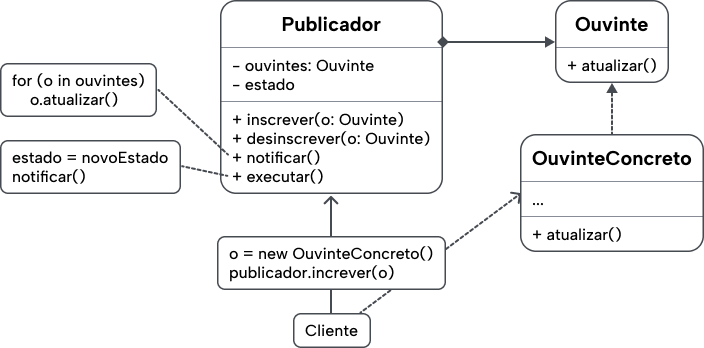
\includegraphics[width=.65\textwidth]{figures/design_patterns/observer_diagram.png}
    \caption{Diagrama da Estrutura do Padrão Observer}
    \label{fig:observer_diagram}
\end{figure}


\subsection{Padrão de Projeto State}

\subsection{Padrão de Projeto Builder}

Segundo \citeonline{GOF}, o padrão de projeto \textit{Builder} permite a separação da construção de um objeto complexo da sua representação, de forma que o mesmo processo de construção pode criar diferentes representações. O padrão organiza a construção do objeto em um conjunto de passos, de modo que, para criar um objeto, é realizada a chamada apenas dos passos necessários(não necessariamente todos) no objeto \textit{builder} e, ao final, é chamado um método que irá realizar de fato a construção do objeto desejado.

Para casos em que um mesmo processo de construção pode ter múltiplas implementações, é possível criar diferentes clases \textit{builder} que implementam o mesmo conjunto de de processos de construção. Para realizar o gerenciamento de diversas implementações de um mesmo processo de construção, o padrão de projeto especifica a existência de uma classe Diretor, que tem a responsabilidade de manejar quais os passos de construção a serem chamados para cada implementação, como pode ser visto na Figura \ref{fig:builder_diagram}

\begin{figure}[ht]
    \centering
    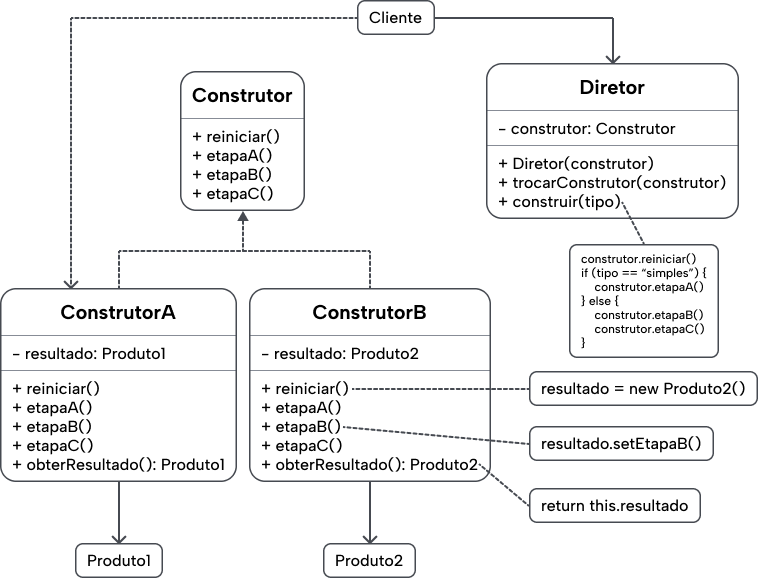
\includegraphics[width=.65\textwidth]{figures/design_patterns/builder_diagram.png}
    \caption{Diagrama da Estrutura do Padrão Builder}
    \label{fig:builder_diagram}
\end{figure}

\subsection{Padrão de Projeto Adapter}

\subsection{Padrão de Projeto Factory}

\subsection{Padrão de Projeto Repository}
O padrão \textit{Repository} foi introduzido por Eric Evans em 2004, por meio da obra \textit{Domain Driven Design}. Esse padrão provê uma interface que abstrai o acesso a dados de uma aplicação, de forma que é possível adicionar, remover, atualizar e buscar dados de uma dada coleção sem tenha-se a preocupação com especificidades de onde os dados estão armazenados, já que esses detalhes de como manipular os dados na base de dados estarão presentes apenas na implementação dessa interface. Assim, esse padrão permite um menor acoplamento e faz com que os objetos do domínio da aplicação sejam independentes dos detalhes de persistência.

\section{Domain Driven Design}
Segundo \citeonline{FOWLER3}, a ideia da necessidade de sistemas de software serem baseados em um modelo de domínio bem desenvolvido é algo presente na indústria à muito tempo, sendo um ponto chave dos trabalho das comunidades de bancos de dados e de linguagens orientadas a objetos entre os anos 1980 e 1990. Um dos trabalhos com maior destaque para resolver essa necessidade da indústria foi o \textit{Domain Driven Design}, introduzido por \citeonline{EVANS} em seu livro "Domain-driven design: atacando as complexidades no coração do software", lançado em 2003.

O \textit{Domain Driven Design(DDD)} se caracteriza como uma abordagem de desenvolvimento que focaliza na criação de um modelo de domínio que tenha um entendimento rico dos processo e regras de um domínio. Segundo \citeonline{VERNON}, um modelo de domínio é um modelo de software do domínio de negócio específico do qual se está trabalhando, de forma a normalmente ser representado por meio de um modelo de objeto que possui dados e comportamentos com significado literal e preciso do negócio em questão. Assim, para praticar o DDD é essencial criar um modelo de domínio único e cuidadosamente trabalhado nas necessidades do negócio, além de ter-se sempre a noção de que os modelos de domínio devem pequenos e muito focados, de forma a nunca buscar representar todo o domínio de negócio em um único e grande modelo de domínio.

Um aspecto de grande importância introduzido pelo DDD é a existência de uma linguagem universal no processo de desenvolvimento de software. \citeonline{EVANS} coloca em sua obra com central a existência dos especialistas de domínio na criação de um projeto de software. Essas pessoas são caracterizadas por terem o conhecimento a cerca do que o projeto precisa e o conhecimento do segmento de negócio que a aplicação de software está envolvida. Assim, a linguagem universal tida por \citeonline{EVANS} se coloca como a linguagem comum que deve ser compartilhada por toda equipe, tanto os desenvolvedores quanto os especialistas do domínio, de forma a diminuir o atrito na comunicação e a realização de traduções de termos técnicos entre as linguagens de desenvolvimento e de negócio.

De forma a materializar a linguagem universal e o modelo de domínio, o DDD introduz os chamados contextos delimitados e os mapas de contexto. Segundo \citeonline{MASOTTI}, como cada área de negócio possui conjuntos de termos diferentes no dia a dia de trabalho de acordo com o contexto inserido, a construção de um modelo de domínio unificado se torna uma tarefa complexa. Assim, os contextos delimitados colaboram no processo de desenvolvimento ao estabelecer limites e dividir o grandes modelos em contextos menores, com a criação de inter-relacionamento entre eles. Em conjunto com os contextos delimitados, têm-se os mapas de contextos, que atua como uma visão geral da modelagem desenvolvida, de forma a facilitar o entendimento dos contextos da aplicação. Esse documento criado deve abranger a relação entre os contextos delimitados de uma organização, de modo a colaborar com o entendimento da equipe sobre o domínio de negócio, as fronteiras entre os contextos e como essas fronteiras podem ser integradas.

Dentro do DDD, a ideia de linguagem universal, modelo de domínio, contextos delimitados e mapas de contexto se une sobre o que é colocado por \citeonline{EVANS} como design estratégico, que visa estabelecer limites e responsabilidades claras na construção da topologia de alto nível de um software. Uma próxima etapa no DDD é a caracterizada como design tático, que foca nos detalhes de implementação e tem como foco refinar o design estratégico por meio de padrões de abstração de médio e baixo nível e auxiliar na construção do código final.

O design tático colabora no momento de codificação do modelo de domínio, a partir das definições colocadas pelo design estratégico anteriormente, de forma que ele se divide em dois grupos: os Modelos de Domínio e os Serviços de Domínio. O primeiro busca representar o problema sendo resolvido, no qual são criados padrões para a representação dos objetos de domínio, como entidades, agregados e objetos de valor. Já os serviços de domínio se caracterizam como as estruturas que auxiliarão os Modelos de Domínio em situações mais complexas que os modelo de domínio não conseguem realizar as suas ações, como no caso de acesso a dados em serviços externos.

\section{Hexagonal Architecture}
A arquitetura hexagonal é uma proposta de arquitetura de software introduzida por \citeonline{COCKBURN} em 2005, em uma tentativa de evitar que desenvolvedores caiam em uma problemas estruturais já conhecidos no projeto de softwares orientados a objetos. O principal objetivo do autor é o de permitir que uma aplicação possa ser igualmente utilizada por usuários, programas, testes e \textit{scripts} automatizados e que a aplicação possa ser desenvolvida e testada de forma totalmente isolada de seus dispositivos de tempo de execução e de bancos de dados.

A ideia central da arquitetura hexagonal, também conhecida com arquitetura \textit{port and adapters}, é a de separar o código interno, que conterá as regras de negócio da aplicação, do código externo, que fará a comunicação com vias externas, como bancos de dados e interfaces de usuário. Essa separação se dá por meio da criação de portas na camada de aplicação para que se comunique com agentes externos. A palavra "porta" nesse contexto é com base na ideia de portas de um sistema operacional, em que qualquer dispositivos que adere ao protocolo de uma porta pode se \textit{plugar} a ela. Esses dispositivos que aderem as portas são chamados de adaptadores. Por exemplo, uma aplicação que precisa se comunicar com um meio externo irá criar uma porta para isso, que pode ser implementada por um adaptador que comunica com um banco de dados SQL para trazer os resultados. Se esse banco de dados trocado por um armazenamento em arquivo ou um banco de dados NoSQL, iria-se ter um novo adaptador que iria se \textit{plugar} com a aplicação, mantendo o contrato previamente estabelecido.

Ainda nessa ideia da criação de adaptadores, \citeonline{COCKBURN} faz a distinção entre adaptadores primário e secundários. Um adaptador primário se caracteriza por dirigir a aplicação, atuando como entrada de dados nela, em muitos casos sendo o meio pelo qual o usuário acessa a aplicação, como por meio de uma interface GUI ou por chamadas HTTP. Já o adaptador secundário age ao prover para aplicação dados que ela pode precisar para responder à uma interação feita por um adaptador primário, de forma a atuar na saída de dados, normalmente acessando um banco de dados ou interagindo com algum serviço externo para solicitar algum dado.

\section{Clean Architecture}
Após anos na indústria de desenvolvimento de software, \citeonline{MARTIN2} percebeu o surgimento de muitas arquiteturas de sistemas sendo desenvolvidas, com a maioria delas variando um poucos nos detalhes de implementação, mas sendo muito semelhantes em sua essência, com foco na independência de \textit{frameworks} externos, testabilidade, independência de interface de usuário, bancos de dados ou de qualquer outro agente externo.

Assim, \citeonline{MARTIN2} definiu um modelo geral de como se ter uma arquitetura mais limpa, que não fosse "suja" de detalhes externos que não interessam ao cerne da aplicação e à regra de negócio em questão. Esse modelo é representado por algumas camadas, de forma que existe uma regra de dependência, na qual as dependências de código devem apontar sempre para dentro. Dessa forma, qualquer função, classe, variável ou entidade de software que reside em uma camada interna não deve, em hipótese alguma, saber da existência de uma entidade pertencente a uma camada mais externa.

Na camada mais central da arquitetura limpa se encontram as entidades, que são responsáveis por representar as regras de negócio da organização, que podem ser objetos com métodos ou apenas um conjunto de estruturas de dados e funções. As entidades representam as regras gerais de mais alto nível e são a menos passíveis de mudar em caso de algo externo alterar.

Na próxima camada, tem-se os casos de uso, que representam as regras de negócio da aplicação e orquestram o fluxo de dados de e para as entidades, de forma a fazer as entidades executarem suas regras de negócio da organização de modo a atingir os objetivos dos casos de uso. Qualquer mudança externa também não deve alterar essas camada, porém mudanças nas entidades ou na forma que a aplicação opera irão afetar o software presente nessa camada.

A camada seguinte é a de adaptadores de interface. Essa camada é responsável por ter um conjunto de adaptadores que irão converter os dados da forma mais conveniente em relação aos casos de uso e entidades para a forma mais conveniente para agentes externos, como bancos de dados e a web, e vice-versa. Os modelos nessa camada são apenas estruturas de dados representacionais que irão ser passadas pelas estruturas do software, como funções e classes.

Na camada mais externa proposta por \citeonline{MARTIN2}, tem-se a camada de \textit{Frameworks} e \textit{Drivers}, que é composta pela implementação de \textit{frameworks} e ferramentas como bancos de dados, web, etc. Nessa camada se encontram todos os detalhes da aplicação e, no máximo, se encontra código que irá servir como ponte para se comunicar com a camada mais interna.

\section{Flutter e Dart}
Para demonstrar as boas e más práticas na arquitetura e desenvolvimento de software, será criada uma aplicação de exemplo. Para a construção dela, foi utilizada a linguagem Dart, apresentada pelo Google em 2011, em conjunto com o \textit{framework} Flutter para a criação das partes relacionadas a interface gráfica. A linguagem Dart é uma linguagem de código aberto do paradigma orientado a objetos e se destaca por:
\begin{itemize}
    \item Ser otimizada para \textit{User Interface}
    \item Ter um ambiente de desenvolvimento produtivo, contando com funcionalidades como \textit{Hot Reload}, que permite realizar mudanças iterativamente e visualizar resultados na alteração de código sem que ele precise ser compilado novamente do zero
    \item Estar disponível em diversas plataformas, permitindo compilar para código de máquina ARM e x64 para plataformas móveis, \textit{desktop} e \textit{backend}, além de compilar para JavaScript para a web.
\end{itemize}
Já o \textit{framework} Flutter, criado também pela Google, e apresentado inicialmente em 2015, tem como objetivo permitir a construção de aplicações compiladas de forma nativa e multi plataforma a partir de uma mesma base de código, se caracterizando como um \textit{framework cross-platform}. Para permitir tais capacidades, o Flutter utiliza do Dart como sua linguagem de programação base.



\chapter{Desenvolvimento}
Nesta seção serão abordados alguns problemas comuns no desenvolvimento de aplicações Flutter, de forma que para cada problema será apresentada uma ou mais resoluções de forma a aplicar padrões de projeto e de arquitetura amplamente conhecidos e já documentados. Por meio desses padrões, busca-se código mais padronizados, legíveis, manuteníveis e que haja uma menor chance de erros serem cometidos pelos desenvolvedores enquanto constroem softwares complexos.

\section{O Problema da Representação de Estados}
Por o framework Flutter ser focado na criação de aplicações cliente, ou seja, que são executadas no dispositivo do usuário, existem muitos casos em que é necessário que haja a comunicação com um servidor para execução de regras de negócio e armazenamento de dados. Essa comunicação é feita por meio de requisições à rede internet e ocorrem de maneira assíncrona, com a resposta dessas requisições demorando algum tempo para acontecer. Além disso, essas requisições podem se completar de duas formas: com sucesso e com erro. Em casos de sucesso, costuma-se ter como o resultado a informação que se deseja obter do servidor, ou então uma confirmação de que o envio de dados foi realizado com sucesso. Em casos de erros, pode-se ter mensagens ou códigos de erro de forma que o usuário possa entender melhor qual o erro que ocorreu ao realizar uma ação dentro da aplicação, já que o erro pode ser causado por motivos diversos, desde um valor inválido informado pelo usuário até erros de comunicação de baixo nível na rede. Esse mesmo princípio pode se aplicar para comunicações que não sejam em rede, como em acessos a bancos de dados no dispositivo do usuário, chamadas de sistema operacional, comunicação por \textit{Bluetooth} e muitas outras.

Com isso em vista, têm-se que qualquer tipo de comunicação assíncrona pode ser representada por meio de um diagrama de estados, em que a partir de um estado inicial, transiciona-se para um estado de carregamento a partir de uma ação do usuário e, após a realização da ação assíncrona, pode-se transicionar para um estado de sucesso ou para um estado de erro, como descrito na Figura \ref{fig:states_diagram}.

\begin{figure}[ht]
    \centering
    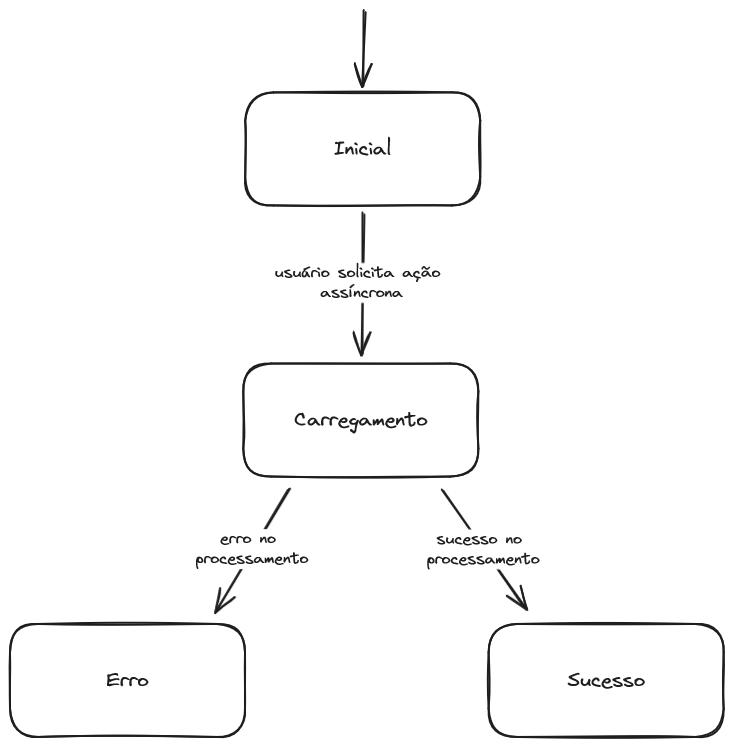
\includegraphics[width=.6\textwidth]{figures/states/states_diagram.png}
    \caption{Diagrama dos estados possíveis em uma ação assíncrona}
    \label{fig:states_diagram}
\end{figure}

Para exemplificar esse mecanismo de realizar uma ação assíncrona a como pode-se melhorá-la, irá ser criada uma tela em que, ao apertar de um botão, será exibido um componente de carregamento e depois de um tempo o conteúdo mudará para um texto de sucesso ou de erro. Para realizar essa simulação de requisição assíncrona, terá-se a função \textit{getInformationFromNetwork}, exibida na Figura \ref{fig:simulate_request}, que irá simular uma ação assíncrona aguardando 2 segundos e, de forma aleatória, jogará uma exceção personalizada com uma mensagem de erro ou retornará uma classe de sucesso, que conterá uma \textit{String} com a informação fictícia que teria sido obtida.

\begin{figure}[ht]
    \centering
    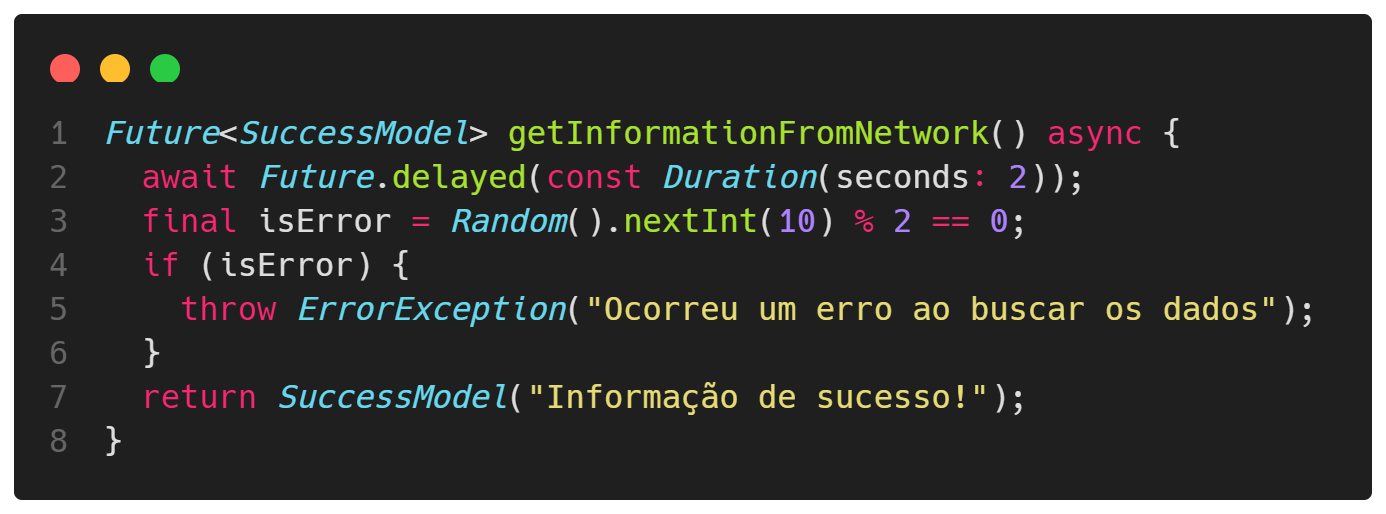
\includegraphics[width=.65\textwidth, trim={0 30 0 100}, clip]{figures/states/getInformationFromNetwork.png}
    \caption{Função para simular uma ação assíncrona}
    \label{fig:simulate_request}
\end{figure}

\subsection{Exemplo Adhoc para Representação de Estados}

Como um exemplo \textit{adhoc}, utilizando o mecanismo mais básico para gerenciamento de estado efêmero do Flutter, o \textit{setState}, pode-se criar dentro de um \textit{StatefulWidget} três variáveis, uma variável booleana para representar o carregamento da requisição, uma \textit{String nullable} com o conteúdo da mensagem de erro e uma variável \textit{nullable} com o objeto de sucesso, como exemplificado na Figura \ref{fig:variables}.

\begin{figure}[ht]
    \centering
    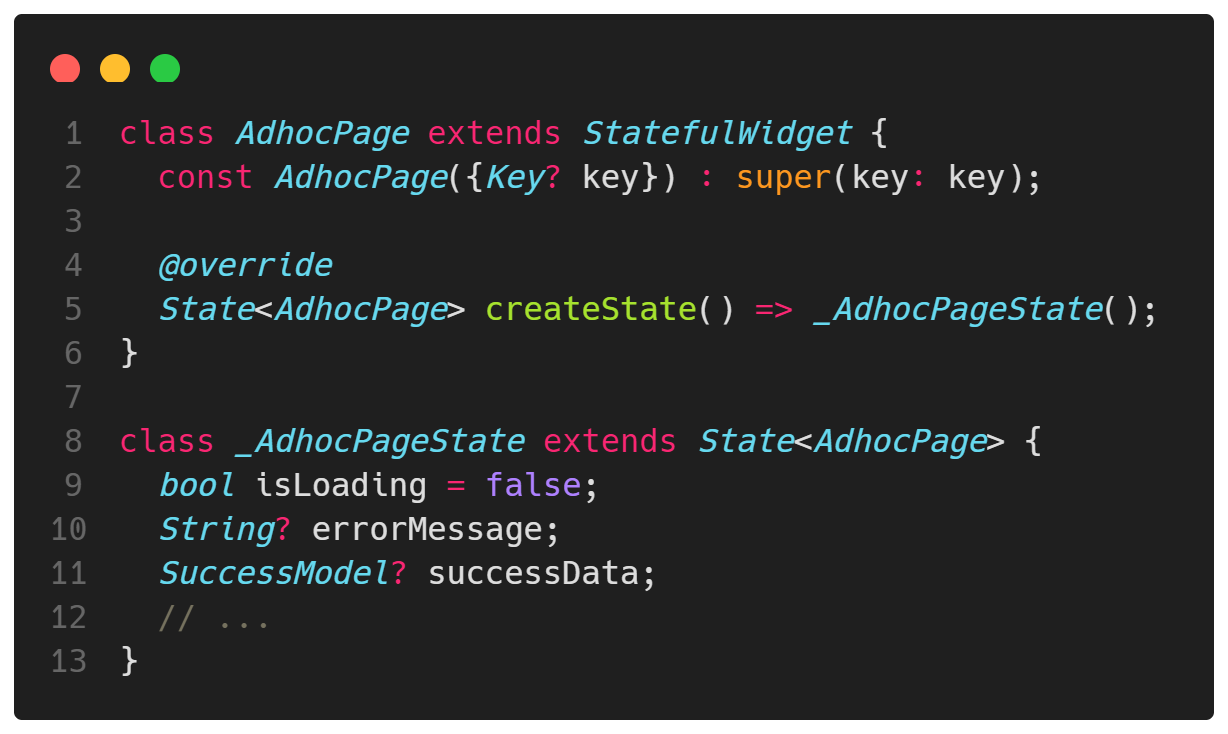
\includegraphics[width=.65\textwidth, trim={0 30 0 100}, clip]{figures/states/variables.png}
    \caption{Variáveis para representar os estados da página}
    \label{fig:variables}
\end{figure}

Em seguida, cria-se a parte visual que tratará por exibir diferentes componentes de acordo com os valores contidos nas variáveis descritas anteriormente. Todo esse trecho de código está presente dentro do método \textit{build} da classe \textit{\_AdhocPageState}, como visto na Figura \ref{fig:adhoc_widget}.

\begin{figure}[ht]
    \centering
    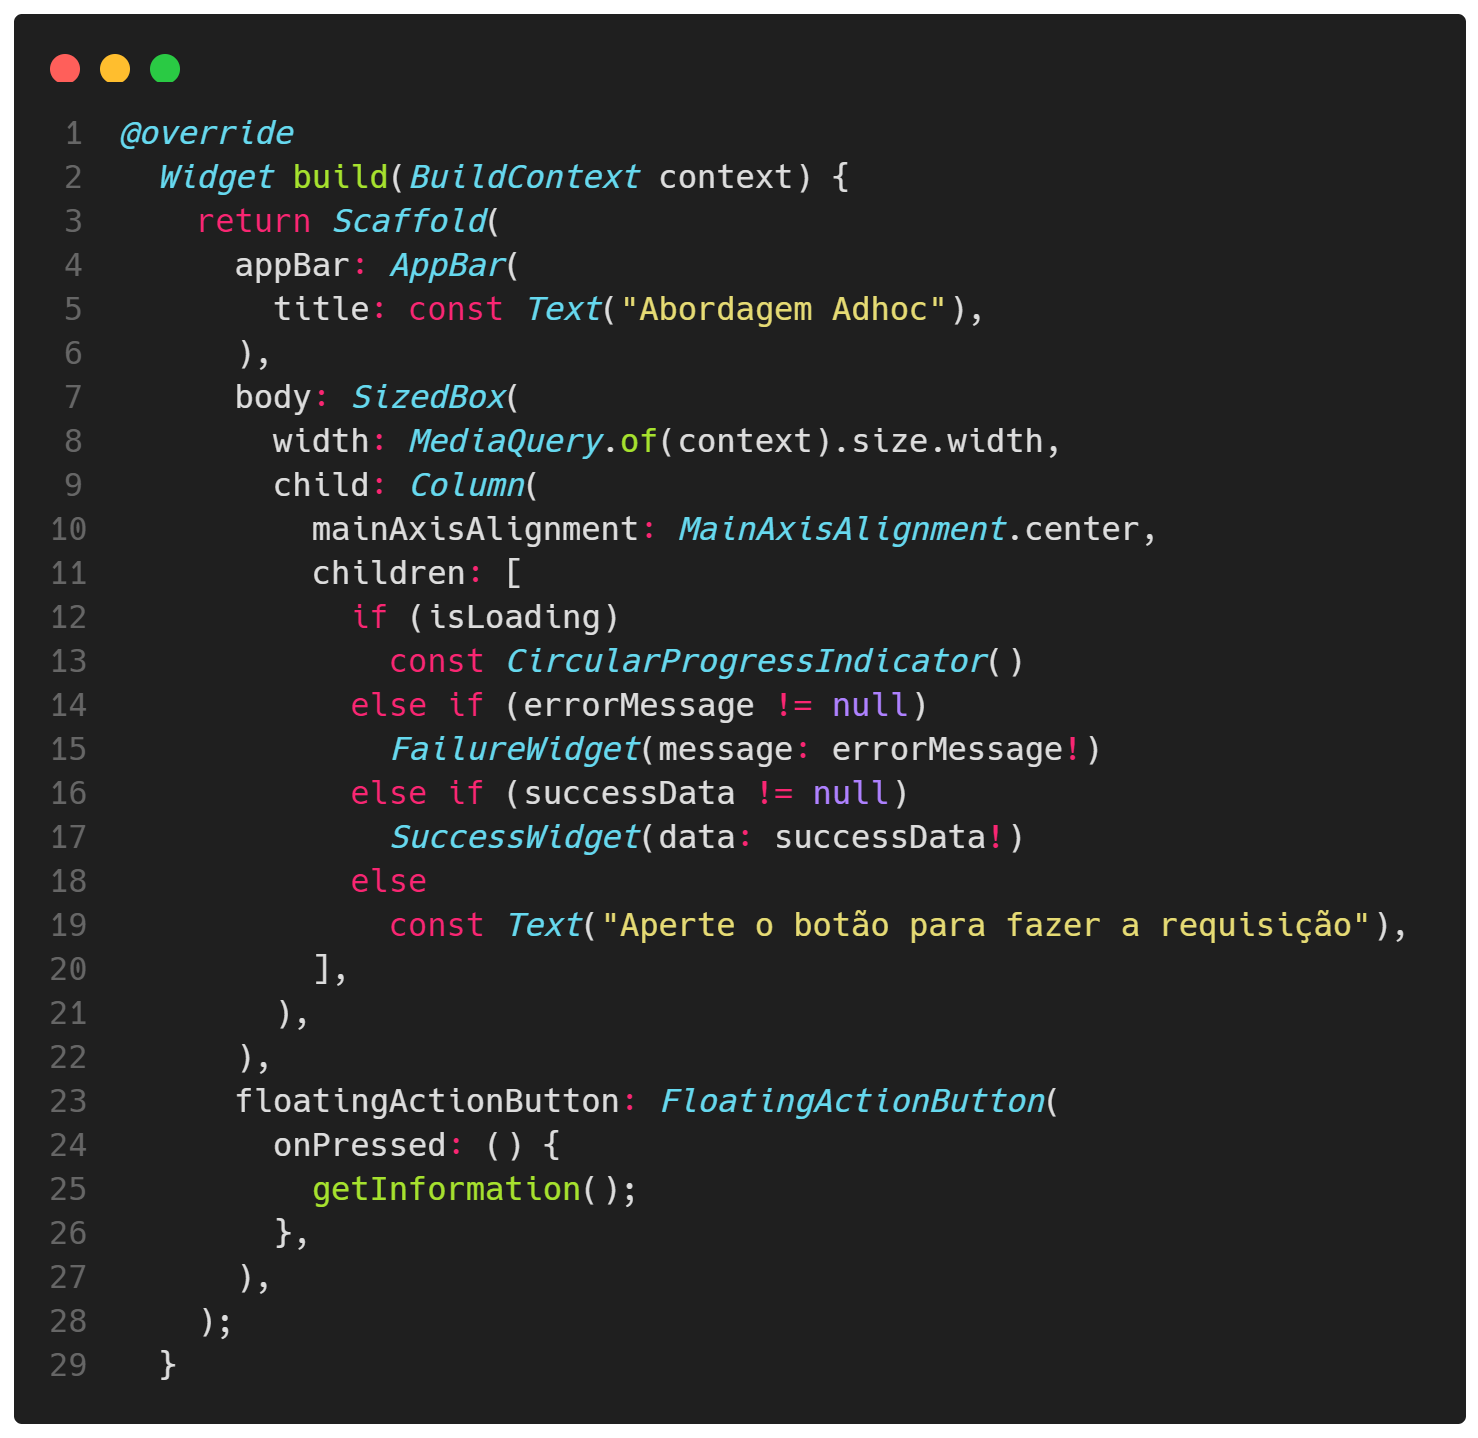
\includegraphics[width=.65\textwidth, trim={0 30 0 100}, clip]{figures/states/adhoc_widget.png}
    \caption{Método \textit{build} para construção da tela da abordagem \textit{adhoc}}
    \label{fig:adhoc_widget}
\end{figure}

Por último nessa classe têm-se a função \textit{getInformation}, que será responsável por alterar as variáveis e fazer a chamada à função que simulará a requisição, visto na Figura \ref{fig:adhoc_getinfo}.

\begin{figure}[ht]
    \centering
    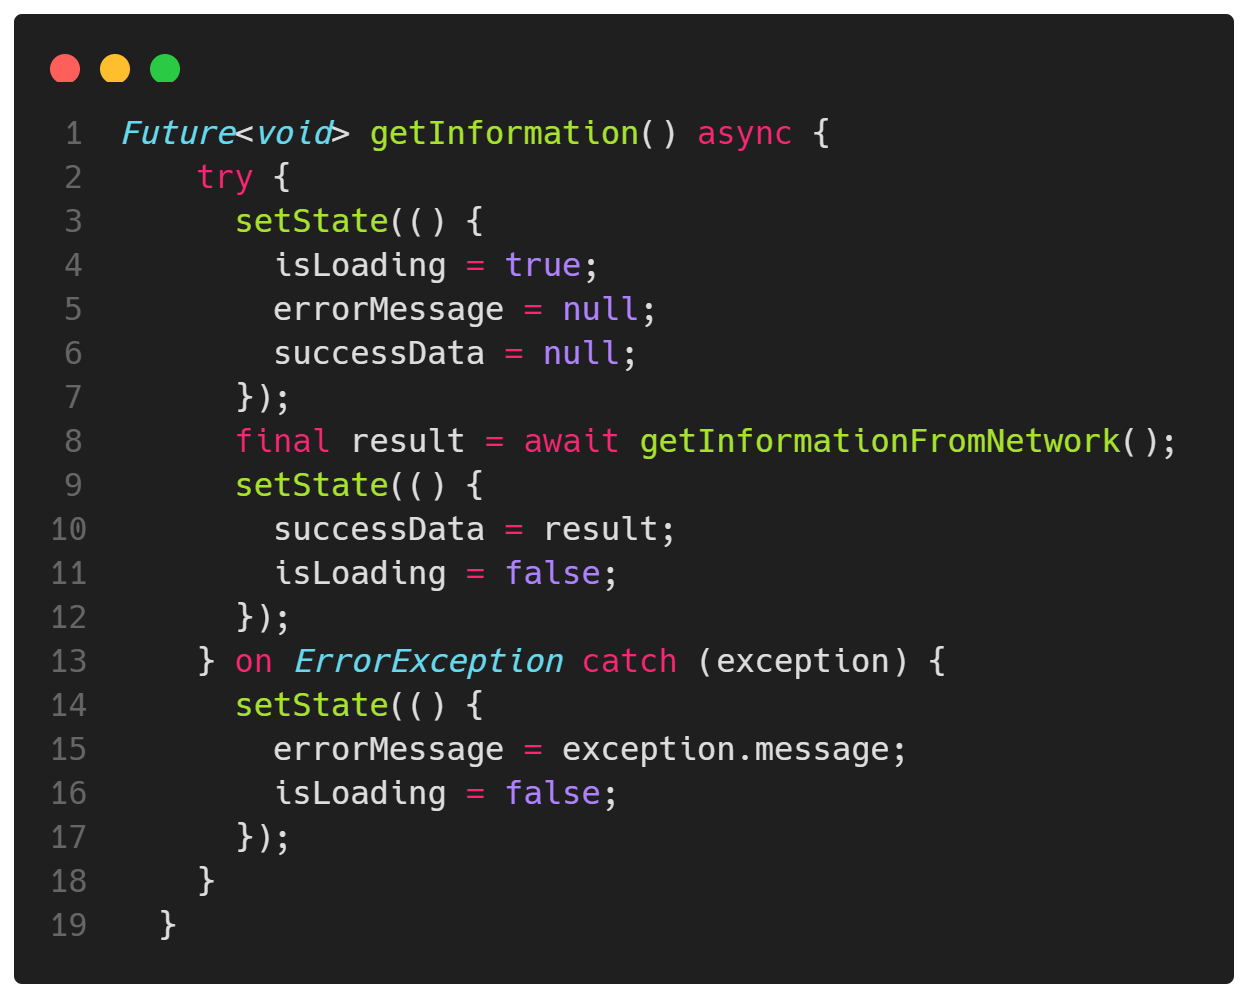
\includegraphics[width=.65\textwidth, trim={0 30 0 100}, clip]{figures/states/adhoc_getinfo.png}
    \caption{Função que realizará a alteração dos estados de acordo com o andamento da ação assíncrona}
    \label{fig:adhoc_getinfo}
\end{figure}

Sobre essa abordagem, embora seja simples e direta, pode-se apontar alguns problemas. Um primeiro problema é a quebra do Princípio da Responsabilidade Única, visto que a classe responsável pela exibição da interface gráfica é também responsável por gerenciar o estado da aplicação. Além disso, a forma apresentada permite a representação de estados inválidos. Por exemplo, é possível de ter a variável \textit{isLoading} com o valor verdadeiro ao mesmo tempo que a variável \textit{successData} não é nula ou então é possível ter ambas as variáveis \textit{successData} e \textit{errorMessage} não nulas ao mesmo tempo. Esses casos e outros são considerados representações inválidas, visto que não estão previstas no diagrama da Figura \ref{fig:states_diagram}, além de ferirem o princípio DRY que afirma que todo pedaço de conhecimento deve ter uma representação única, não ambígua e autoritativa dentro de um sistema. Outro possível problema é que a forma apresentada não força o desenvolvedor a tratar, na parte da interface visual, todos os estados possíveis, de forma que o desenvolvedor pode se esquecer de criar os componentes a serem exibidos para algum dos estados, ou então, caso seja adicionado um estado novo no futuro da aplicação, também é possível que os desenvolvedores não adicionem a tratativa na parte de renderização de tela.

\subsection{Aplicação do Observer Pattern}

Para resolver o primeiro problema, pode-se criar uma classe separada para fazer o gerenciamento do estado da aplicação, de forma que a classe da interface gráfica será responsável apenas por exibir o conteúdo de acordo com o estado atual presente nela. Porém, o método \textit{setState} só está presente dentro do \textit{StatefulWidget} criado, não podendo ser acessado por outras classes. Um meio de resolver esse problema, pode ser feito pela implementação do padrão de projeto \textit{Observer}. Assim, como visto na Figura \ref{fig:notifier}, pode-se criar uma classe \textit{Notifier} que conterá dentro dela uma lista de \textit{callbacks} e os métodos \textit{addListener}, \textit{removeListener} e \textit{notifyListeners} responsáveis por adicionar um ouvinte, remover um ouvinte e notificar todos os ouvintes, respectivamente.

\begin{figure}[ht]
    \centering
    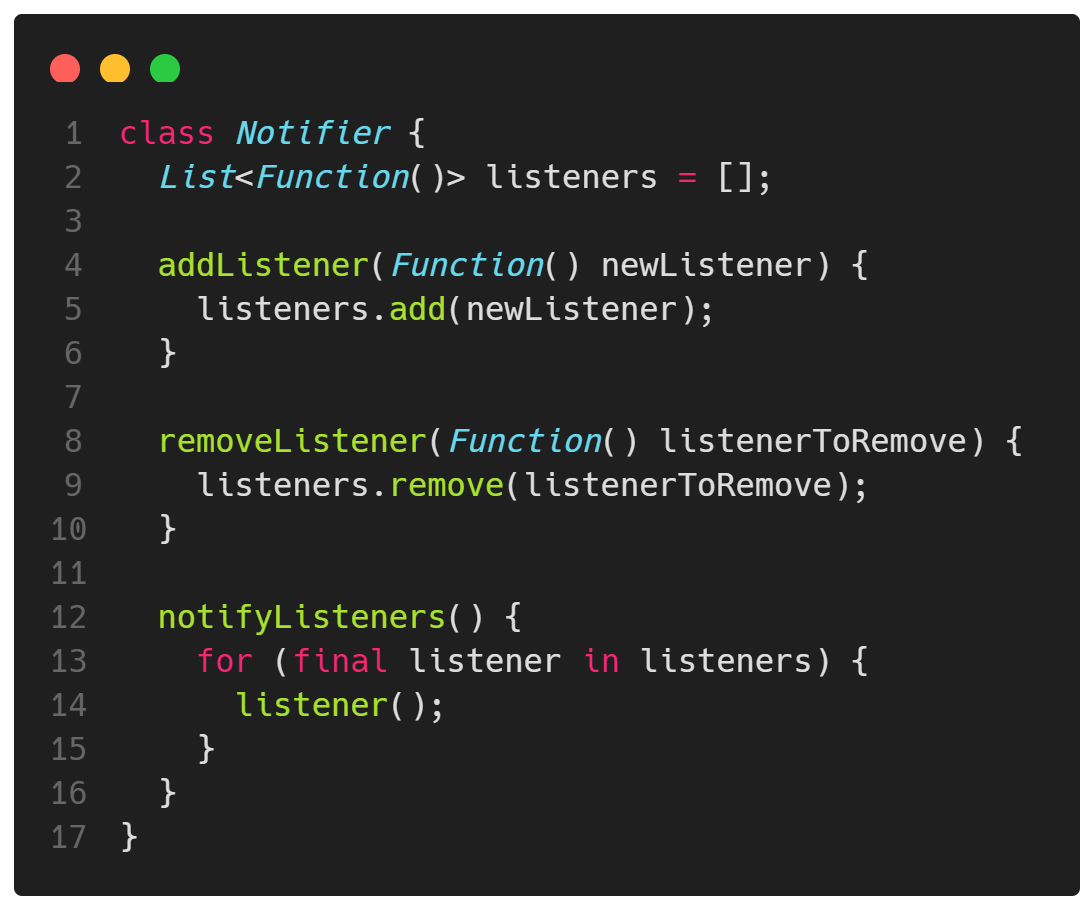
\includegraphics[width=.65\textwidth, trim={0 30 0 100}, clip]{figures/states/notifier.png}
    \caption{Classe \textit{Notifier} que implementa o \textit{Observer Pattern}}
    \label{fig:notifier}
\end{figure}
Para auxiliar no quesito de exibição na tela, podemos criar uma classe \textit{NotifierBuilder}, que será um \textit{StatefulWidget} que receberá uma instância da classe \textit{Notifier} e na sua inicialização chamará o método \textit{addListener} passando uma função anônima que chama a função \textit{setState}, que causará a reconstrução da tela sempre que o método \textit{notifyListeners} for chamado na classe \textit{Notifier}. O código para a classe \textit{NotifierBuilder}, que nada mais é que um ouvinte inscrito na classe publicadora \textit{Notifier}, pode ser visto na Figura \ref{fig:notifier_builder}.

\begin{figure}[ht]
    \centering
    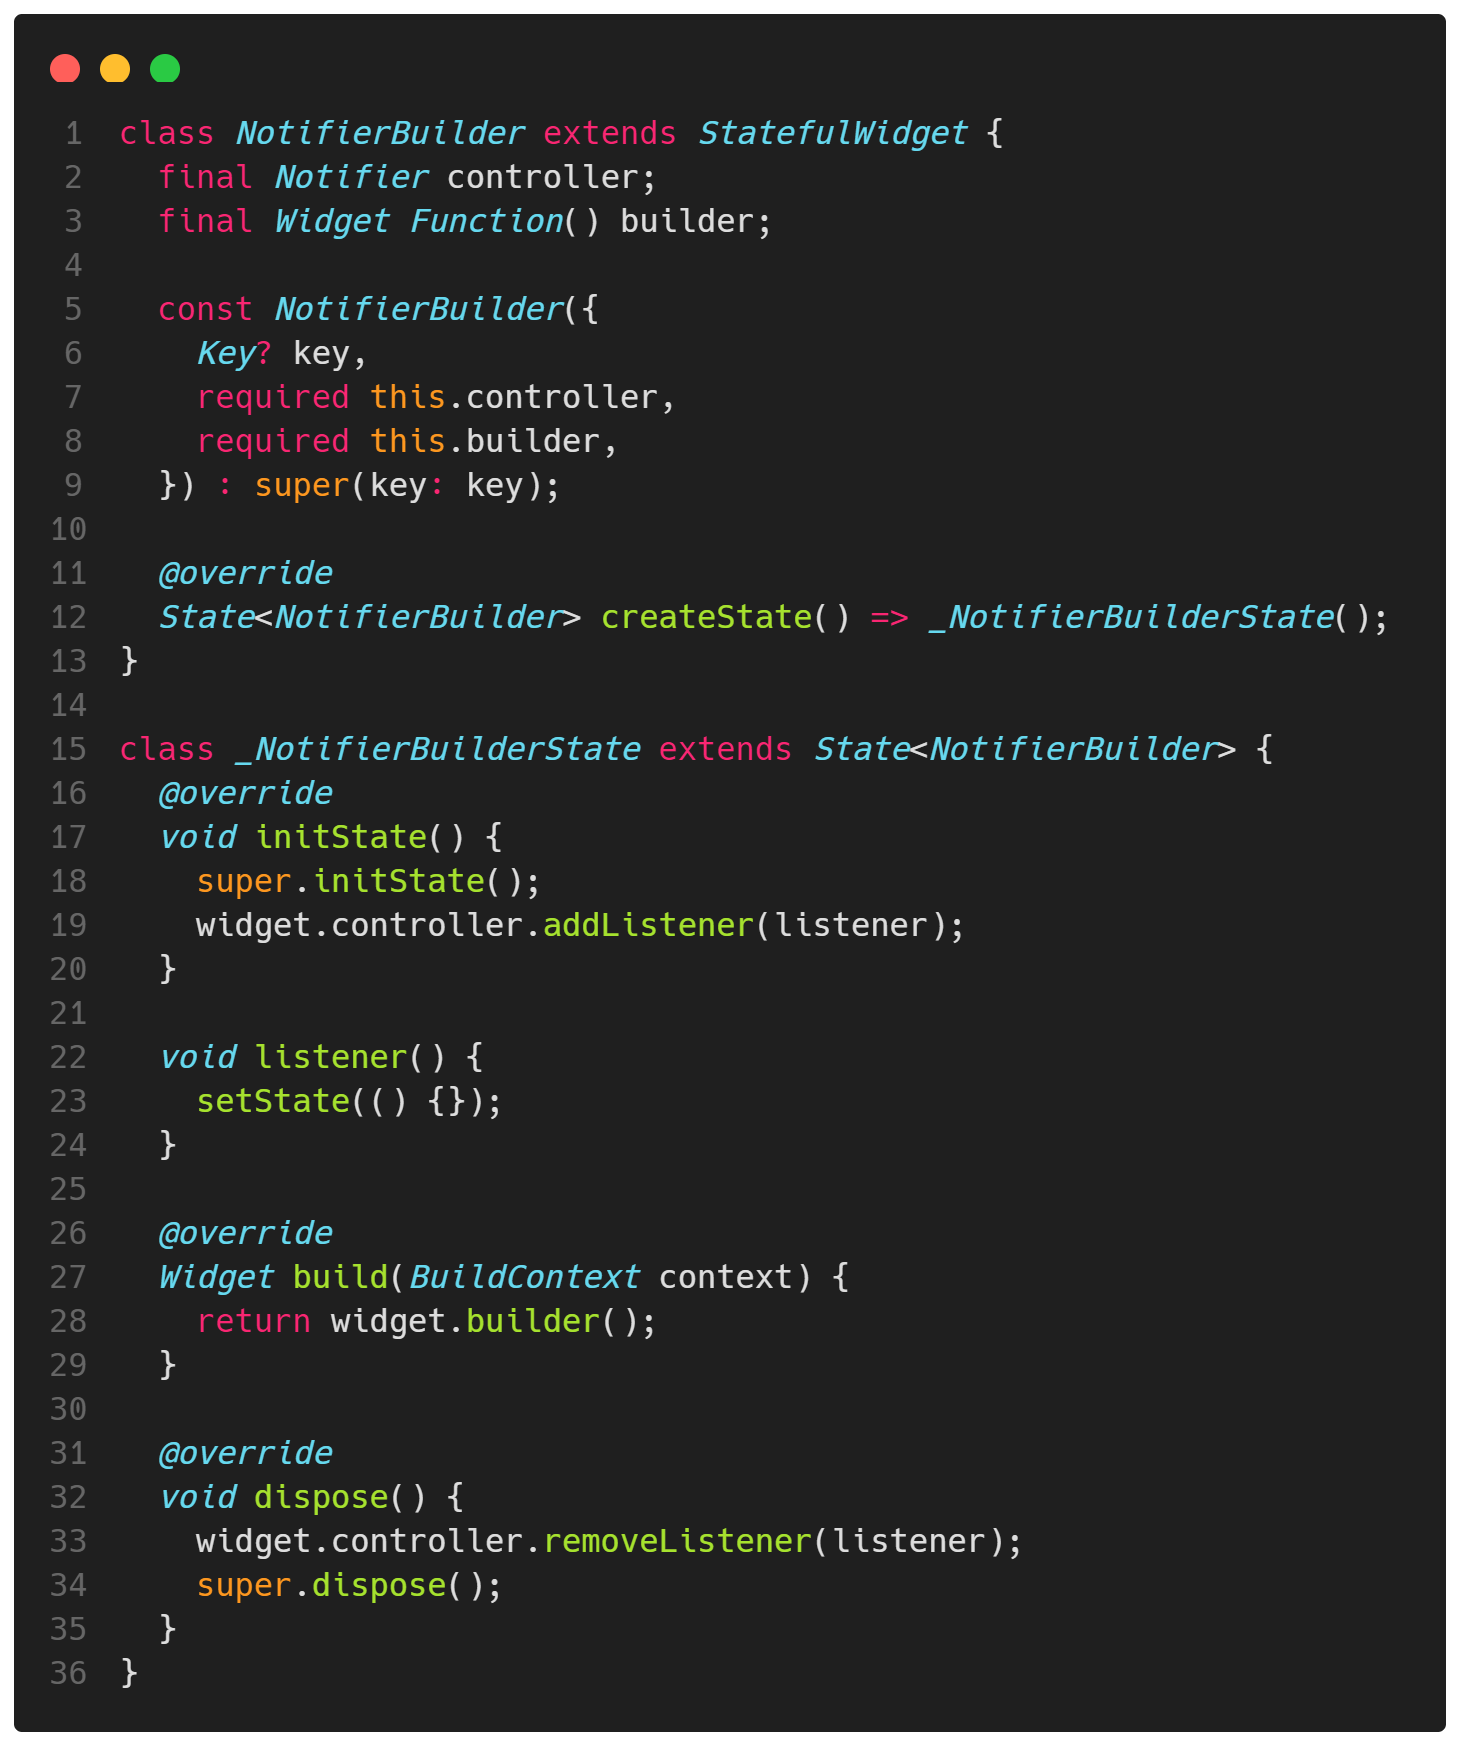
\includegraphics[width=.65\textwidth, trim={0 30 0 100}, clip]{figures/states/notifier_builder.png}
    \caption{Classe \textit{NotifierBuilder}, um ouvinte do \textit{Notifier}}
    \label{fig:notifier_builder}
\end{figure}

Com isso, pode-se criar uma classe que será a nossa controladora de estado e estenderá da classe \textit{Notifier}. Nessa classe \textit{Controller}, têm-se as mesmas variáveis de carregamento, erro e sucesso que antes estavam contidas na classe relativa a UI. Ademais, também está presente nessa classe a função \textit{getInformation}, porém ao invés de usar a função \textit{setState} para acionar a atualização do estado na tela no próximo \textit{frame}, irá ser chamada a função \textit{notifyListeners}, que irá avisar a todos os ouvintes que houve uma alteração e fará com que o ouvinte \textit{NotifierBuilder} chame a função \textit{setState} em seu ouvinte. Além disso, como pode ser visto na Figura \ref{fig:notifier_controller}, as variáveis foram criadas de forma privada e, portanto, foi criado um \textit{getter} para que seja possível que os componentes visuais utilizem os valores das variáveis, mas não os modifiquem.

\begin{figure}[ht]
    \centering
    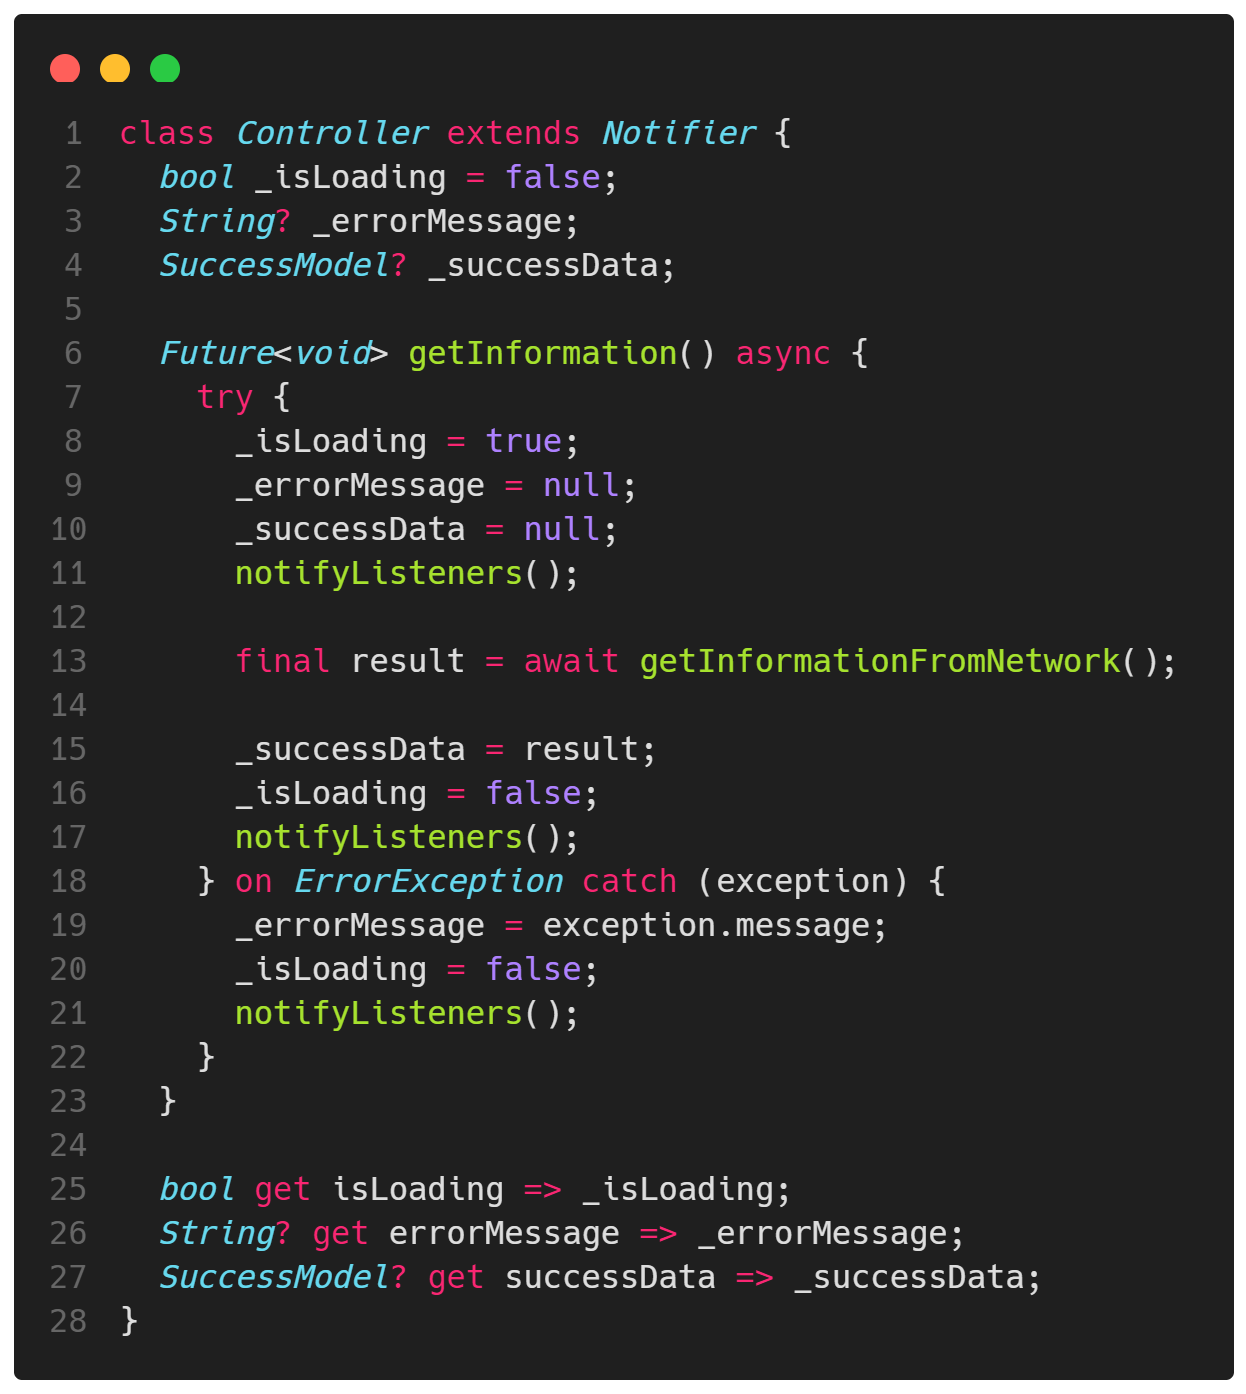
\includegraphics[width=.65\textwidth, trim={0 30 0 100}, clip]{figures/states/notifier_controller.png}
    \caption{Classe \textit{Controller}, responsável por gerenciar o estado da aplicação}
    \label{fig:notifier_controller}
\end{figure}

Com isso, basta reescrever a parte da interface gráfica para passar a utilizar essa classe \textit{Controller}, com o resultado sendo o mostrado na Figura \ref{fig:with_notifier_page}.

\begin{figure}[ht]
    \centering
    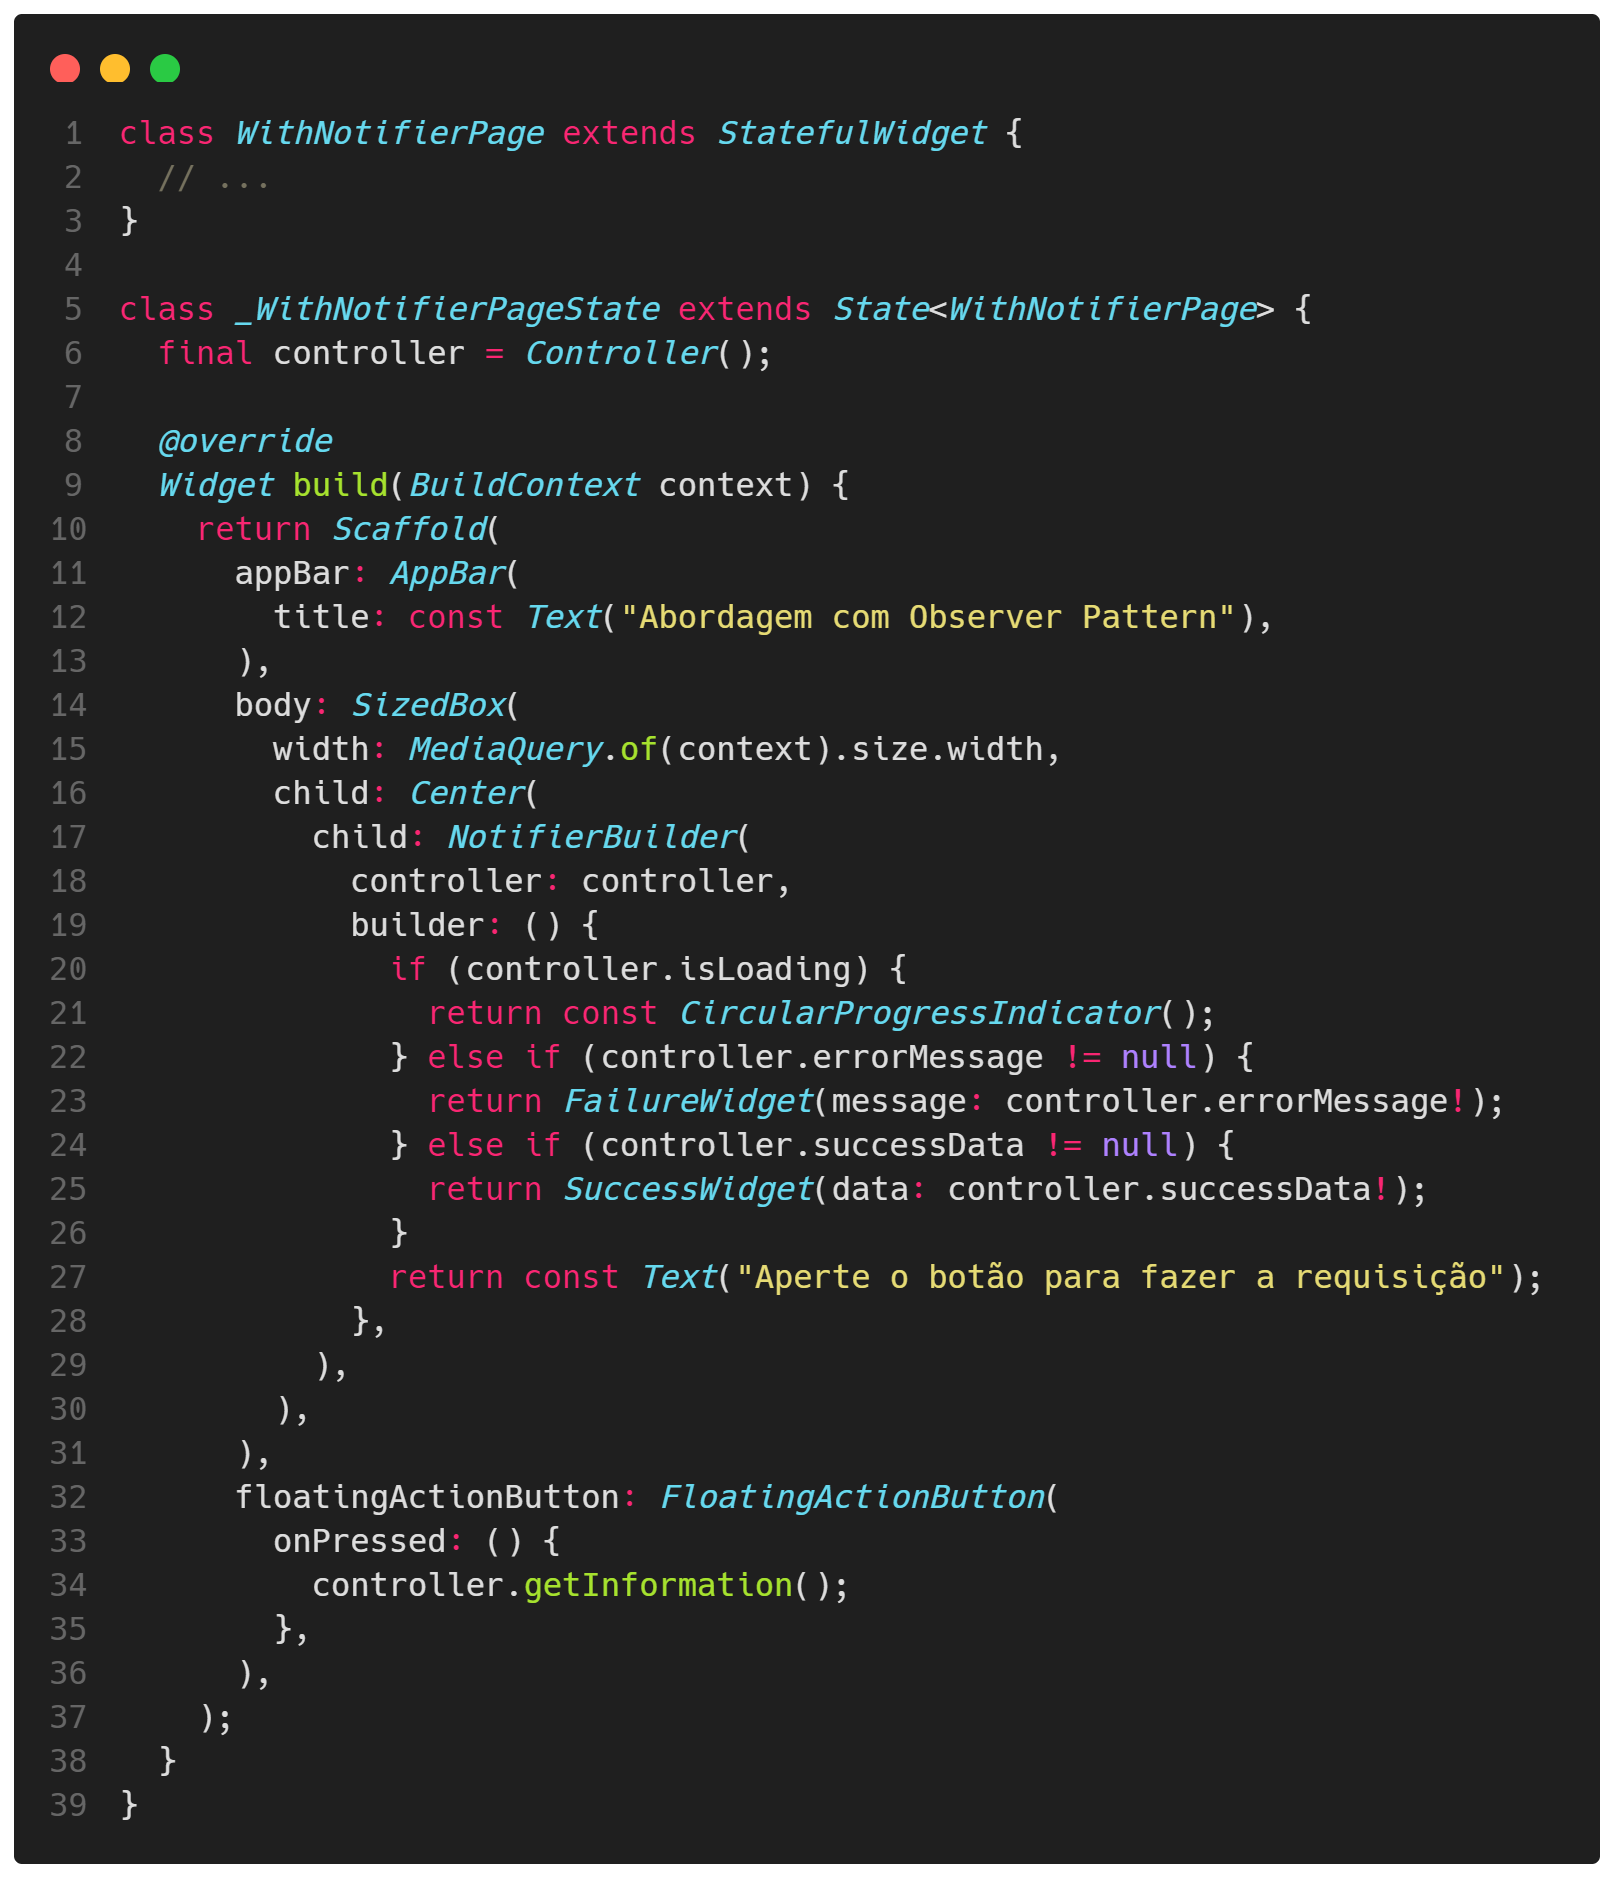
\includegraphics[width=.65\textwidth, trim={0 30 0 100}, clip]{figures/states/with_notifier_page.png}
    \caption{Código da UI utilizando o \textit{Controller} criado}
    \label{fig:with_notifier_page}
\end{figure}

Assim, com a implementação do padrão de projeto \textit{Observer} temos que todo código referente a alteração de estado e obtenção dos dados pela ação assíncrona ficam separados da parte do código de construção da interface. Porém, ainda têm-se o problema de que pode-se haver a representação de estados inválidos, como descrito anteriormente.

\subsection{Aplicação do State Pattern para Representação de Estados Válidos}

Para resolver a questão dos estados inválidos, pode-se utilizar do padrão de projeto \textit{State} em combinação com polimorfismo para que seja criada uma classe base que represente o estado geral e subclasses que irão representar os reais estados da aplicação: inicial, carregamento, erro e sucesso, como visto na Figura \ref{fig:states}. Assim, os dados de sucesso só estão disponíveis dentro da classe de estado de sucesso e o mesmo é válido para o caso de erro, de forma que esses dados não pode ser acessados de forma errônea quando a aplicação estiver em outro estado.

\begin{figure}[ht]
    \centering
    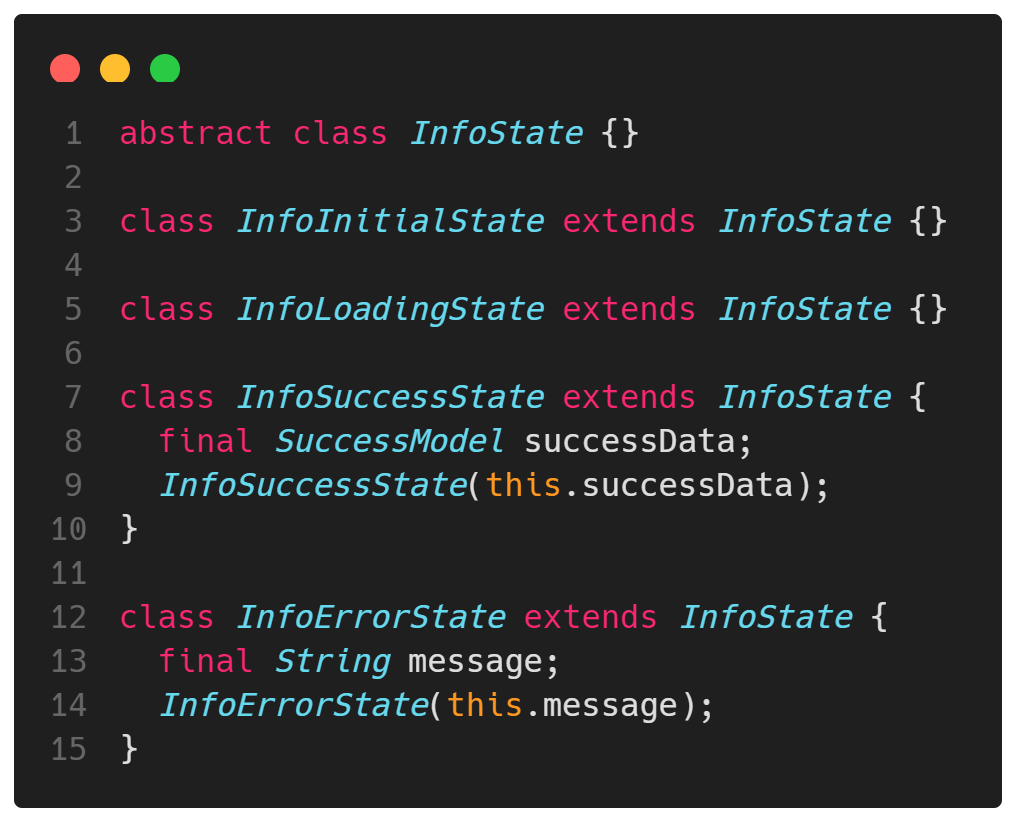
\includegraphics[width=.65\textwidth, trim={0 30 0 100}, clip]{figures/states/states.png}
    \caption{Representação de código utilizando polimorfismo}
    \label{fig:states}

\end{figure}
Com essas classes novas para representar o estado, pode-se refatorar a classe \textit{Controller} para que não seja mais possível haver a representação inválida de múltiplos estados ao mesmo tempo, como era possível anteriormente, além de o código ficar mais enxuto e semântico pela substituição das três variáveis por uma que explicitamente representa o estado da aplicação. Essas alterações podem ser vistas na Figura \ref{fig:controller_with_states}.

\begin{figure}[ht]
    \centering
    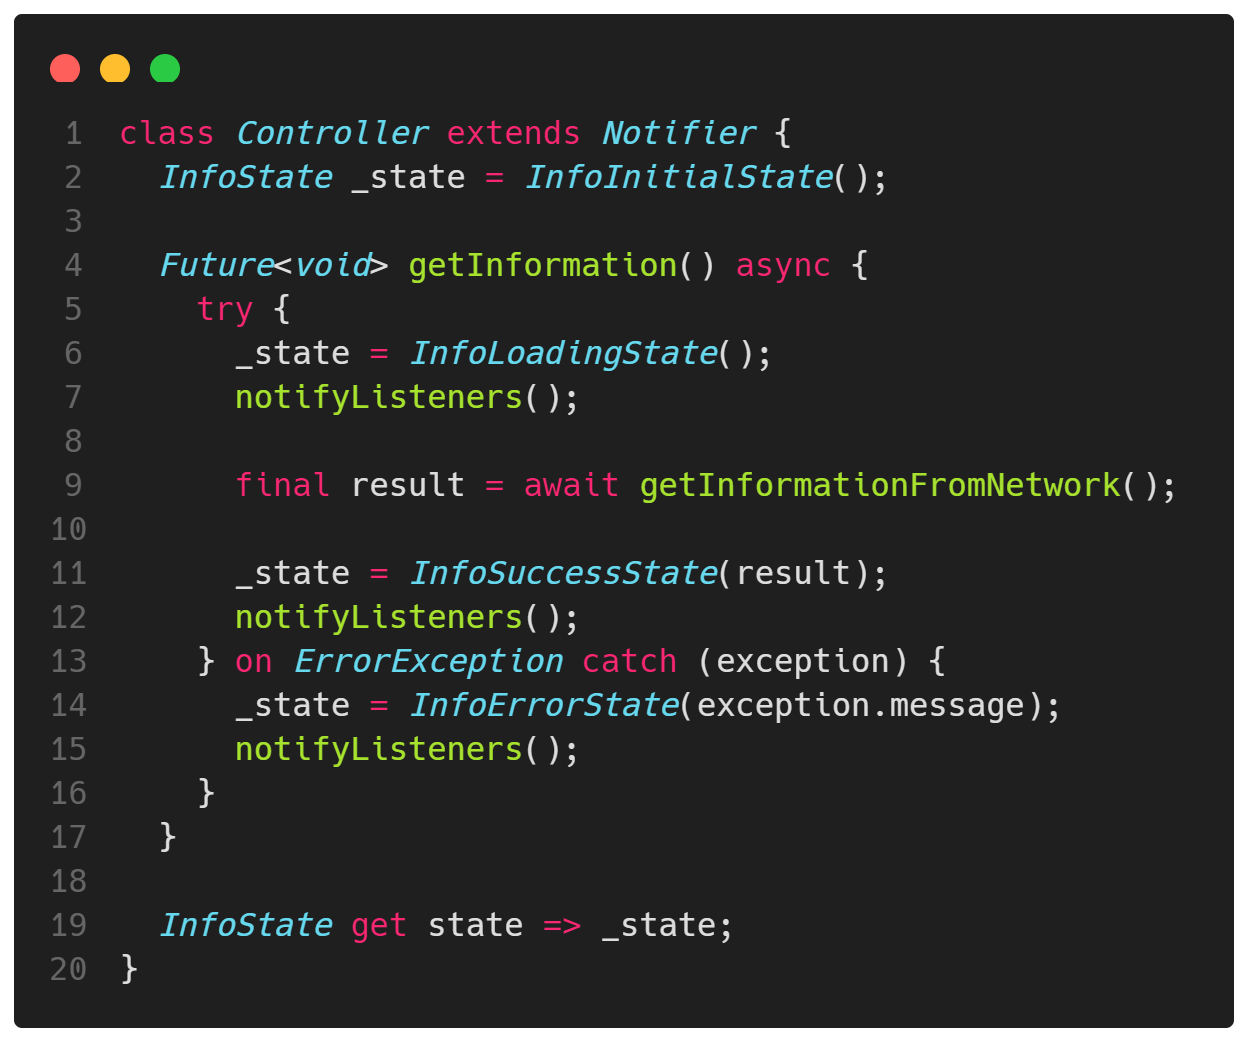
\includegraphics[width=.65\textwidth, trim={0 30 0 100}, clip]{figures/states/controller_with_states.png}
    \caption{Nova versão do \textit{Controller} utilizando as classes de estado criadas}
    \label{fig:controller_with_states}
\end{figure}

Com essa alteração feita, podemos agora alterar a classe da interface para utilizar esses novos estados, fazendo a verificação se a variável \textit{state} do \textit{Controller} é dos subtipos de estado inicial, de carregamento, de erro ou de sucesso, como visto na Figura \ref{fig:with_state_page}.

\begin{figure}[ht]
    \centering
    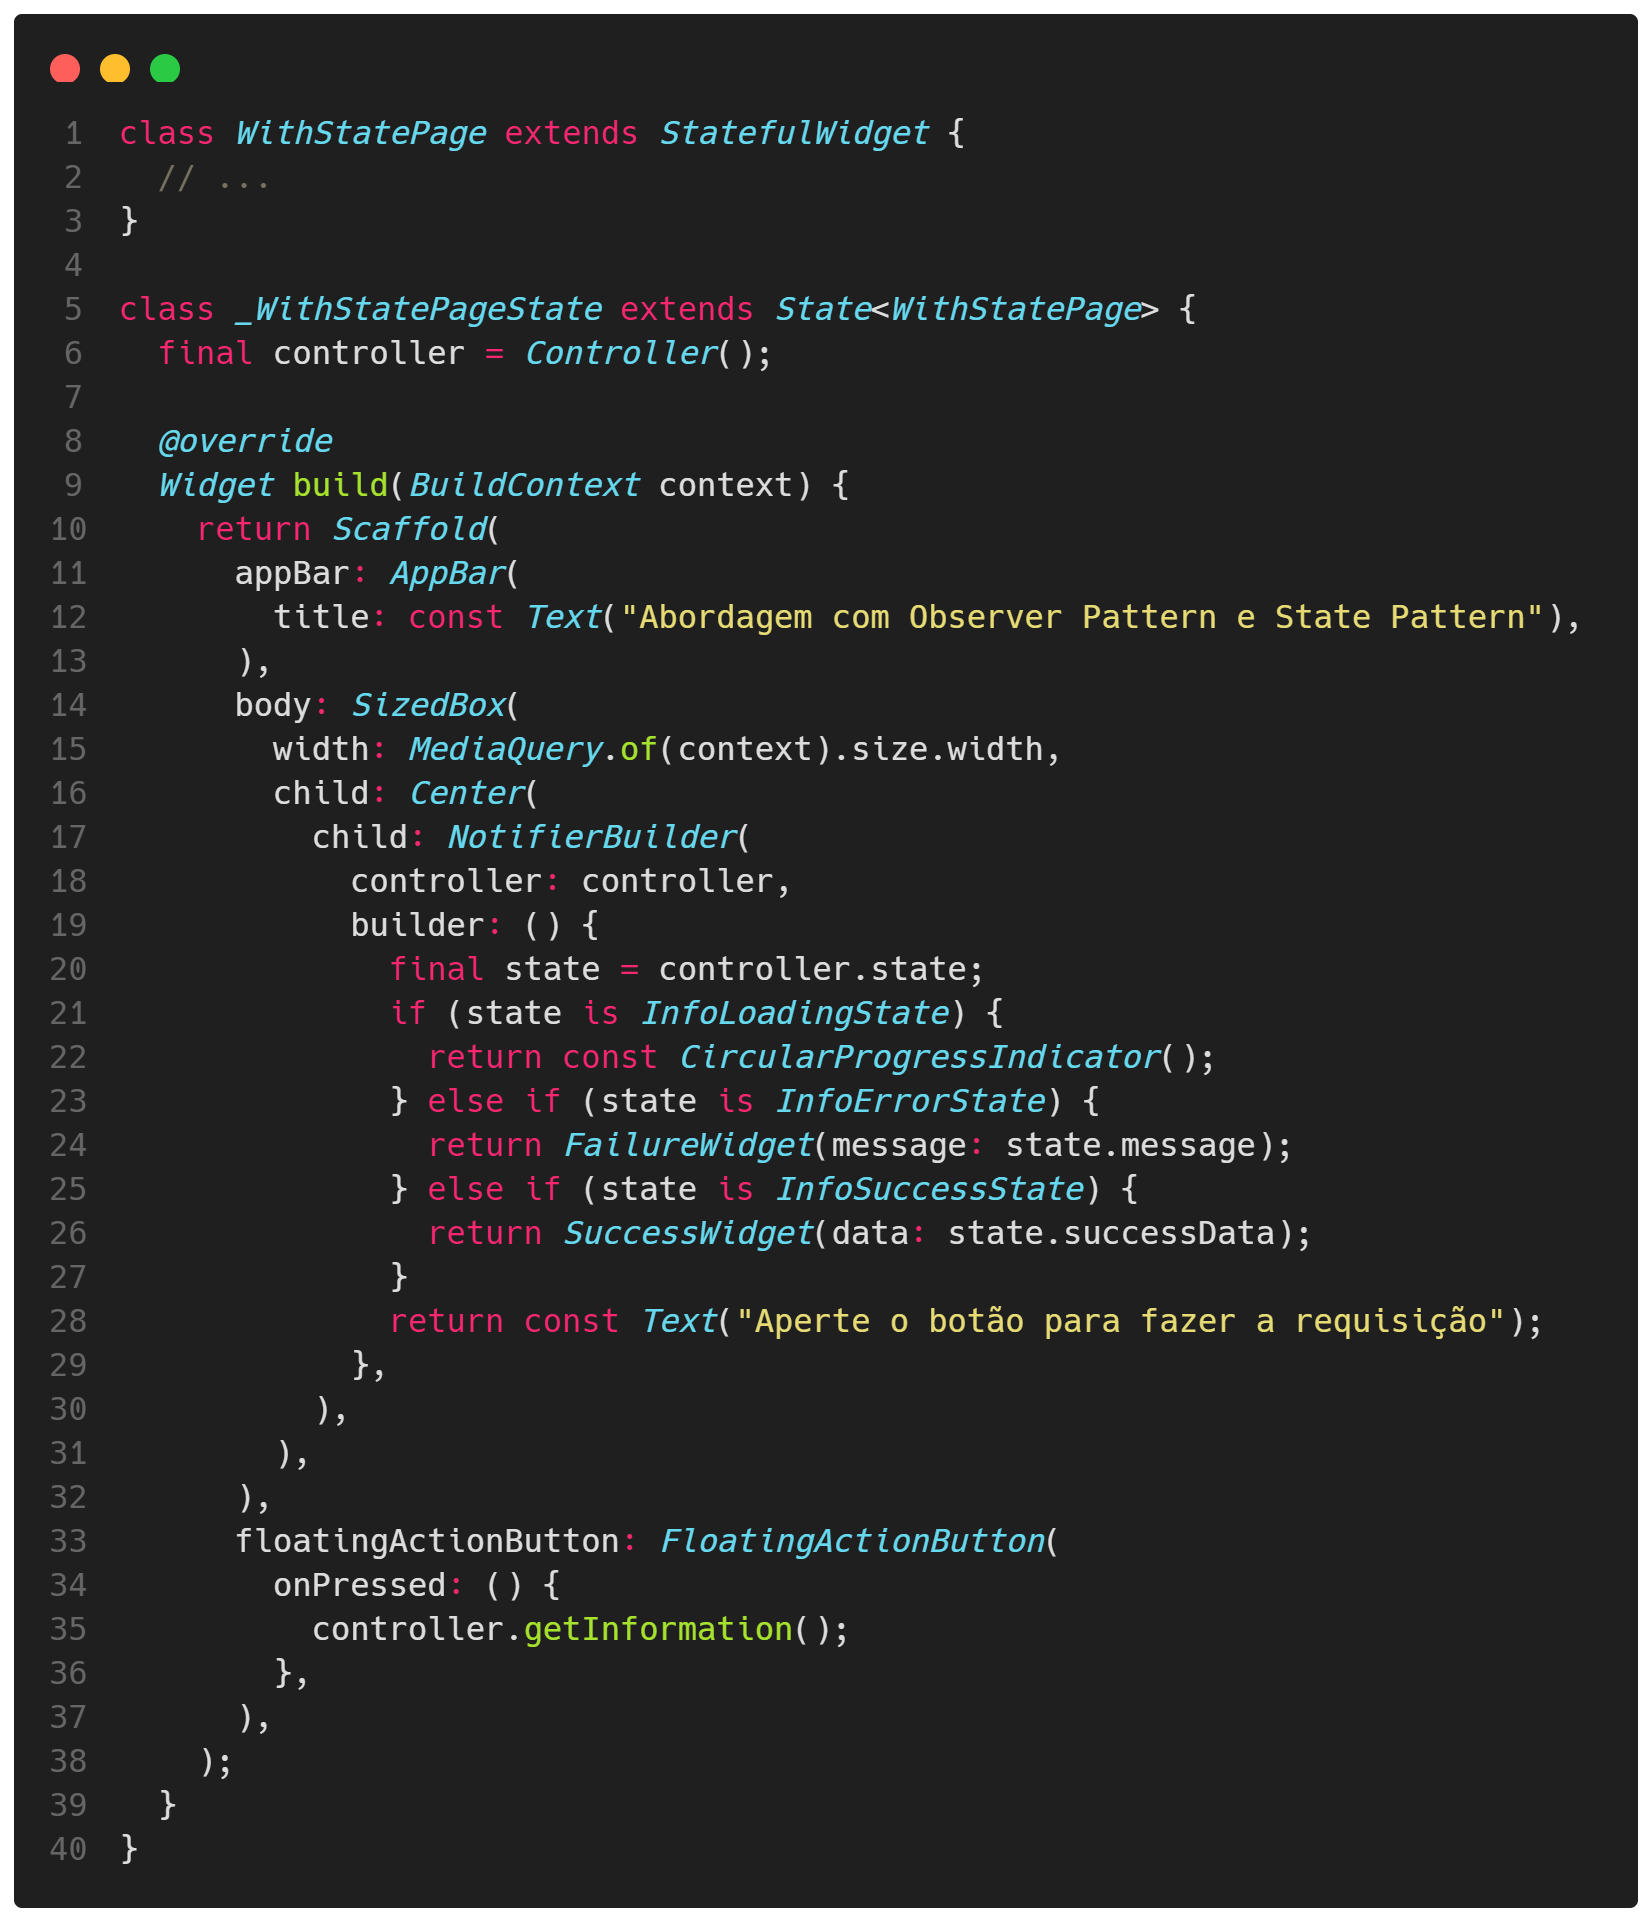
\includegraphics[width=.65\textwidth, trim={0 30 0 100}, clip]{figures/states/with_state_page.png}
    \caption{UI utilizando as classes de estado criadas}
    \label{fig:with_state_page}
\end{figure}

\subsection{Aplicação de Classes Seladas para Match Exaustivo}

Um problema apontado que ainda não foi resolvido é o da possibilidade de o desenvolvedor não tratar todos os estados da aplicação. Isso pode ser resolvido por meio de mecanismos introduzidos pela linguagem Dart em sua versão 3. Nessa versão foram introduzidas classes seladas e várias mecânicas de \textit{pattern matching} na linguagem, que podem ser usadas nas classes de estado apresentadas anteriormente para que, por meio do \textit{pattern matching}, o compilador da linguagem avise sobre estados não tratados. As classes seladas funcionam de forma que elas só podem ser estendidas ou implementadas dentro da mesma biblioteca(e uma biblioteca no Dart é tudo que está dentro de um único arquivo). Dessa forma, o compilador consegue fazer um \textit{match} exaustivo e saber em tempo de compilação todas as subclasses que estendem a classe selada e consegue bloquear a compilação. Na Figura \ref{fig:sealed_states} é mostrada a alteração feita na classe de estado, que deixa de ser abstrata e passa a ser selada. Além disso, às subclasses foi adicionada a palavra reservada \textit{final}, também introduzida na versão 3 da linguagem, para indicar que elas não podem ser estendidas ou implementadas fora da biblioteca, mas podem ser construídas.

\begin{figure}[ht]
    \centering
    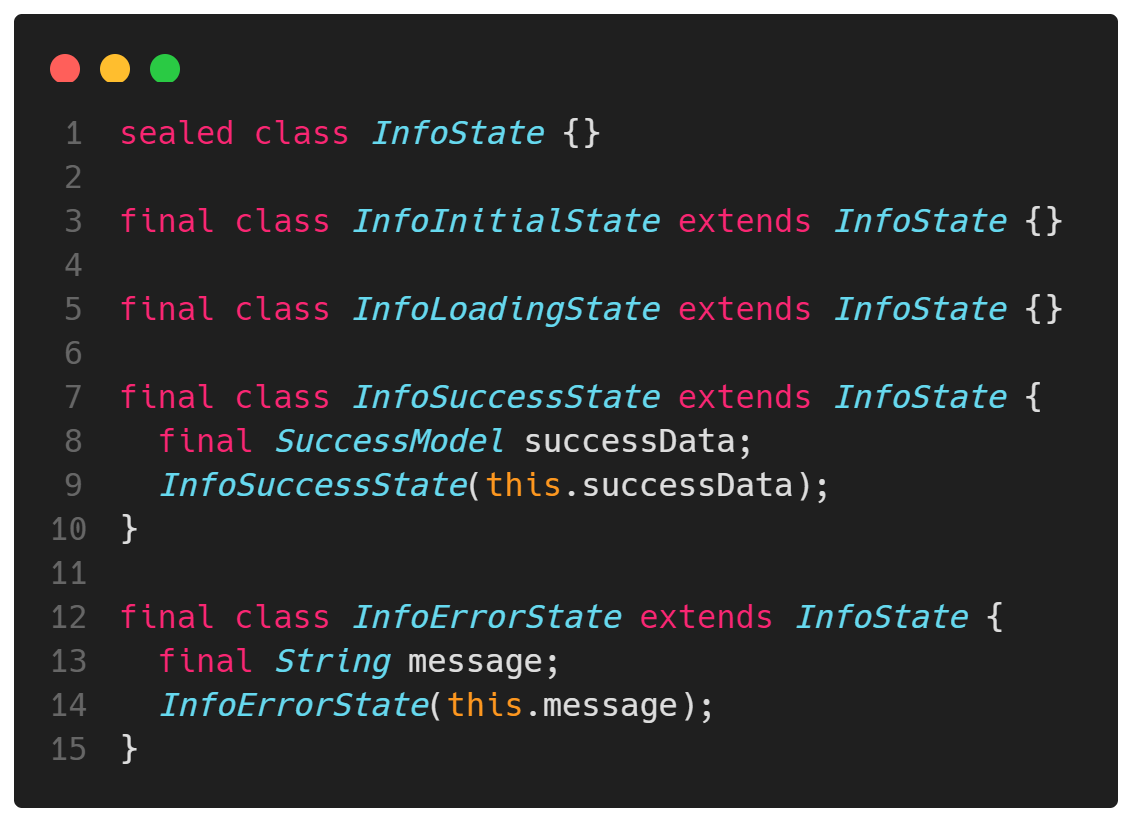
\includegraphics[width=.65\textwidth, trim={0 30 0 100}, clip]{figures/states/sealed_states.png}
    \caption{Alteração nas classes de estados, introduzido o conceito de classes seladas}
    \label{fig:sealed_states}
\end{figure}

Com essa alteração feita nas classes de estados, pode-se alterar a interface da aplicação para que seja feito o \textit{pattern matching} em cima dos possíveis estados da aplicação utilizando a estrutura de \textit{switch-case}, como visto na Figura \ref{fig:sealed_page}, de forma que caso sejam adicionados novos estados no futuro o compilador já irá avisar que não está sendo feito o \textit{match} exaustivo daquela classe, eliminando portanto a chance da aplicação chegar com um \textit{bug} de não ter tratativa de um estado para os usuários.

\begin{figure}[ht]
    \centering
    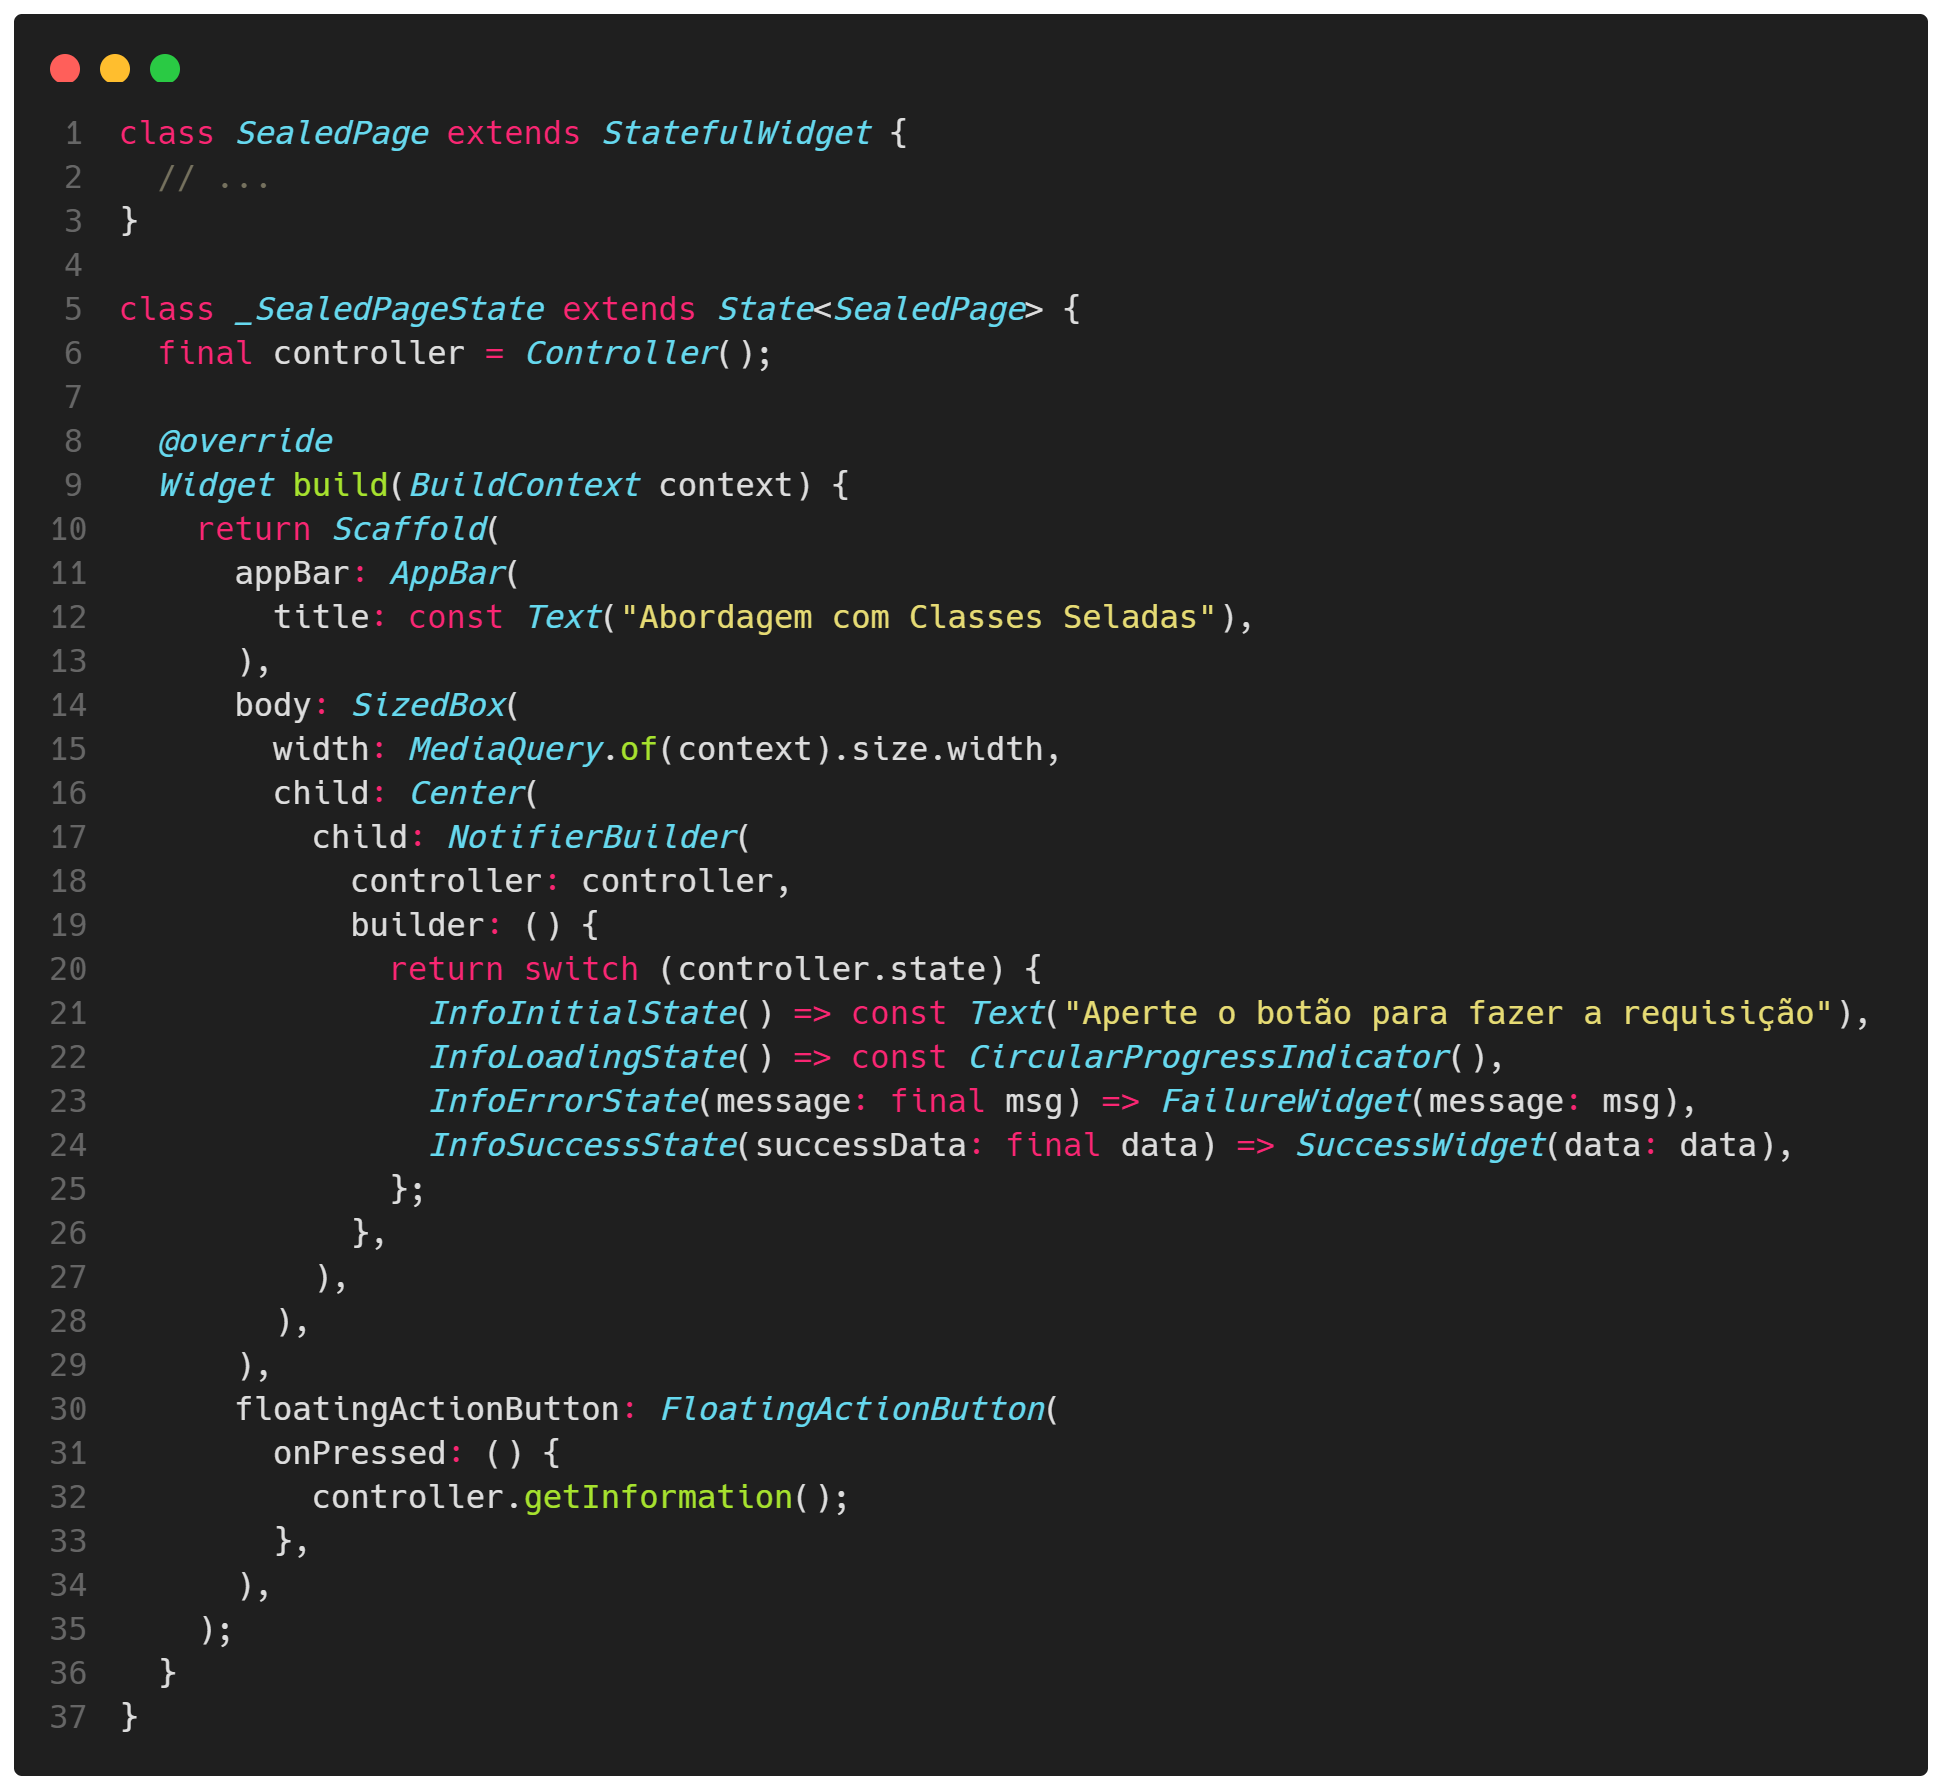
\includegraphics[width=.65\textwidth, trim={0 30 0 100}, clip]{figures/states/sealed_page.png}
    \caption{UI utilizando \textit{pattern matching} para exibição dos componentes de acordo com o estado}
    \label{fig:sealed_page}
\end{figure}

\section{Melhorias para Formulários e suas Validações}

Em aplicações que rodam no lado do cliente, é muito comum a presença de formulários, seja para criação de conta, login, criação de recursos, edição de dados, etc. Para isso, é comum a presença de campos de formulários nessas aplicações, que são componentes de interface que permitem ao usuário digitar valores e registrá-los, seja por um envio desses dados à algum servidor ou pela escrita em um banco de dados no próprio dispositivo.

Assim, além da coleta desses dados pela aplicação cliente, é muito importante haver também a validação desses dados na própria aplicação por dois principais motivos. O primeiro deles se relaciona com a experiência do usuário. Em caso do usuário digitar algo que seja inválido, é importante avisá-lo com boas mensagens de erros que sejam as mais descritivas possível, além de mostrar essas mensagens de erro de forma reativa, ou seja, conforme ele já digita nos campos para que ele já saiba o quanto antes que o valor está incorreto, visto que pode ser uma experiência desagradável para um usuário de uma aplicação só ser avisado sobre erros no formulário somente após preencher diversos campos de formulário. Outro motivo que denota a importância de se haver a validação na própria aplicação é de garantir a consistência de dados do formulário a ser preenchido, de forma que não sejam armazenados dados inválidos. Por exemplo, pode-se garantir que o valor em um campo que deve ser um CPF, seja realmente um CPF válido de acordo com o algoritmo de geração de CPF, ou que um campo que é uma data realmente seja uma data válida, e não uma data que aponte para um mês maior que 12, ou um dia que não existe em um determinado mês.

\subsection{Estruturas Padrões para Lidar com Formulários}

Para lidar com validações de campos de formulário, o Flutter por si só já oferece mecanismos prontos para lidar com isso, por meio do \textit{widget} \textit{TextFormField}, que possui uma propriedade \textit{validator} que permite a execução de uma função anônima que será executada a cada vez que houver uma modificação no campo. Essa função deve retornar \textit{null} em caso do campo estar válido ou uma \textit{String} com a mensagem de error em caso do campo estar inválido. Para que já seja executada a validação conforme o usuário digitar no campo, o framework disponibiliza a propriedade \textit{autovalidateMode}, que pode ser atribuída com o valor \textit{AutovalidateMode.onUserInteraction}. Ainda, para que seja possível obter o valor do campo posteriormente, é necessário criar uma instância de \textit{TextEditingController} para cada campo e adicionar no atributo \textit{controller} de cada \textit{TextFormField}. Ao final de um formulário, é comum ter-se um botão para fazer o registros dos dados e, para que possa-se prosseguir com a ação desejada, o formulário deve estar válido. Para isso, o framework disponibiliza uma classe \textit{Form} que deve envolver os componentes de formulário, de forma que deve ser dada a essa instância uma \textit{key}, do tipo \textit{GlobalKey<FormState>}, que possibilitará a verificação da validade do formulário, como visto na figura \ref{fig:example_form}

\begin{figure}[ht]
    \centering
    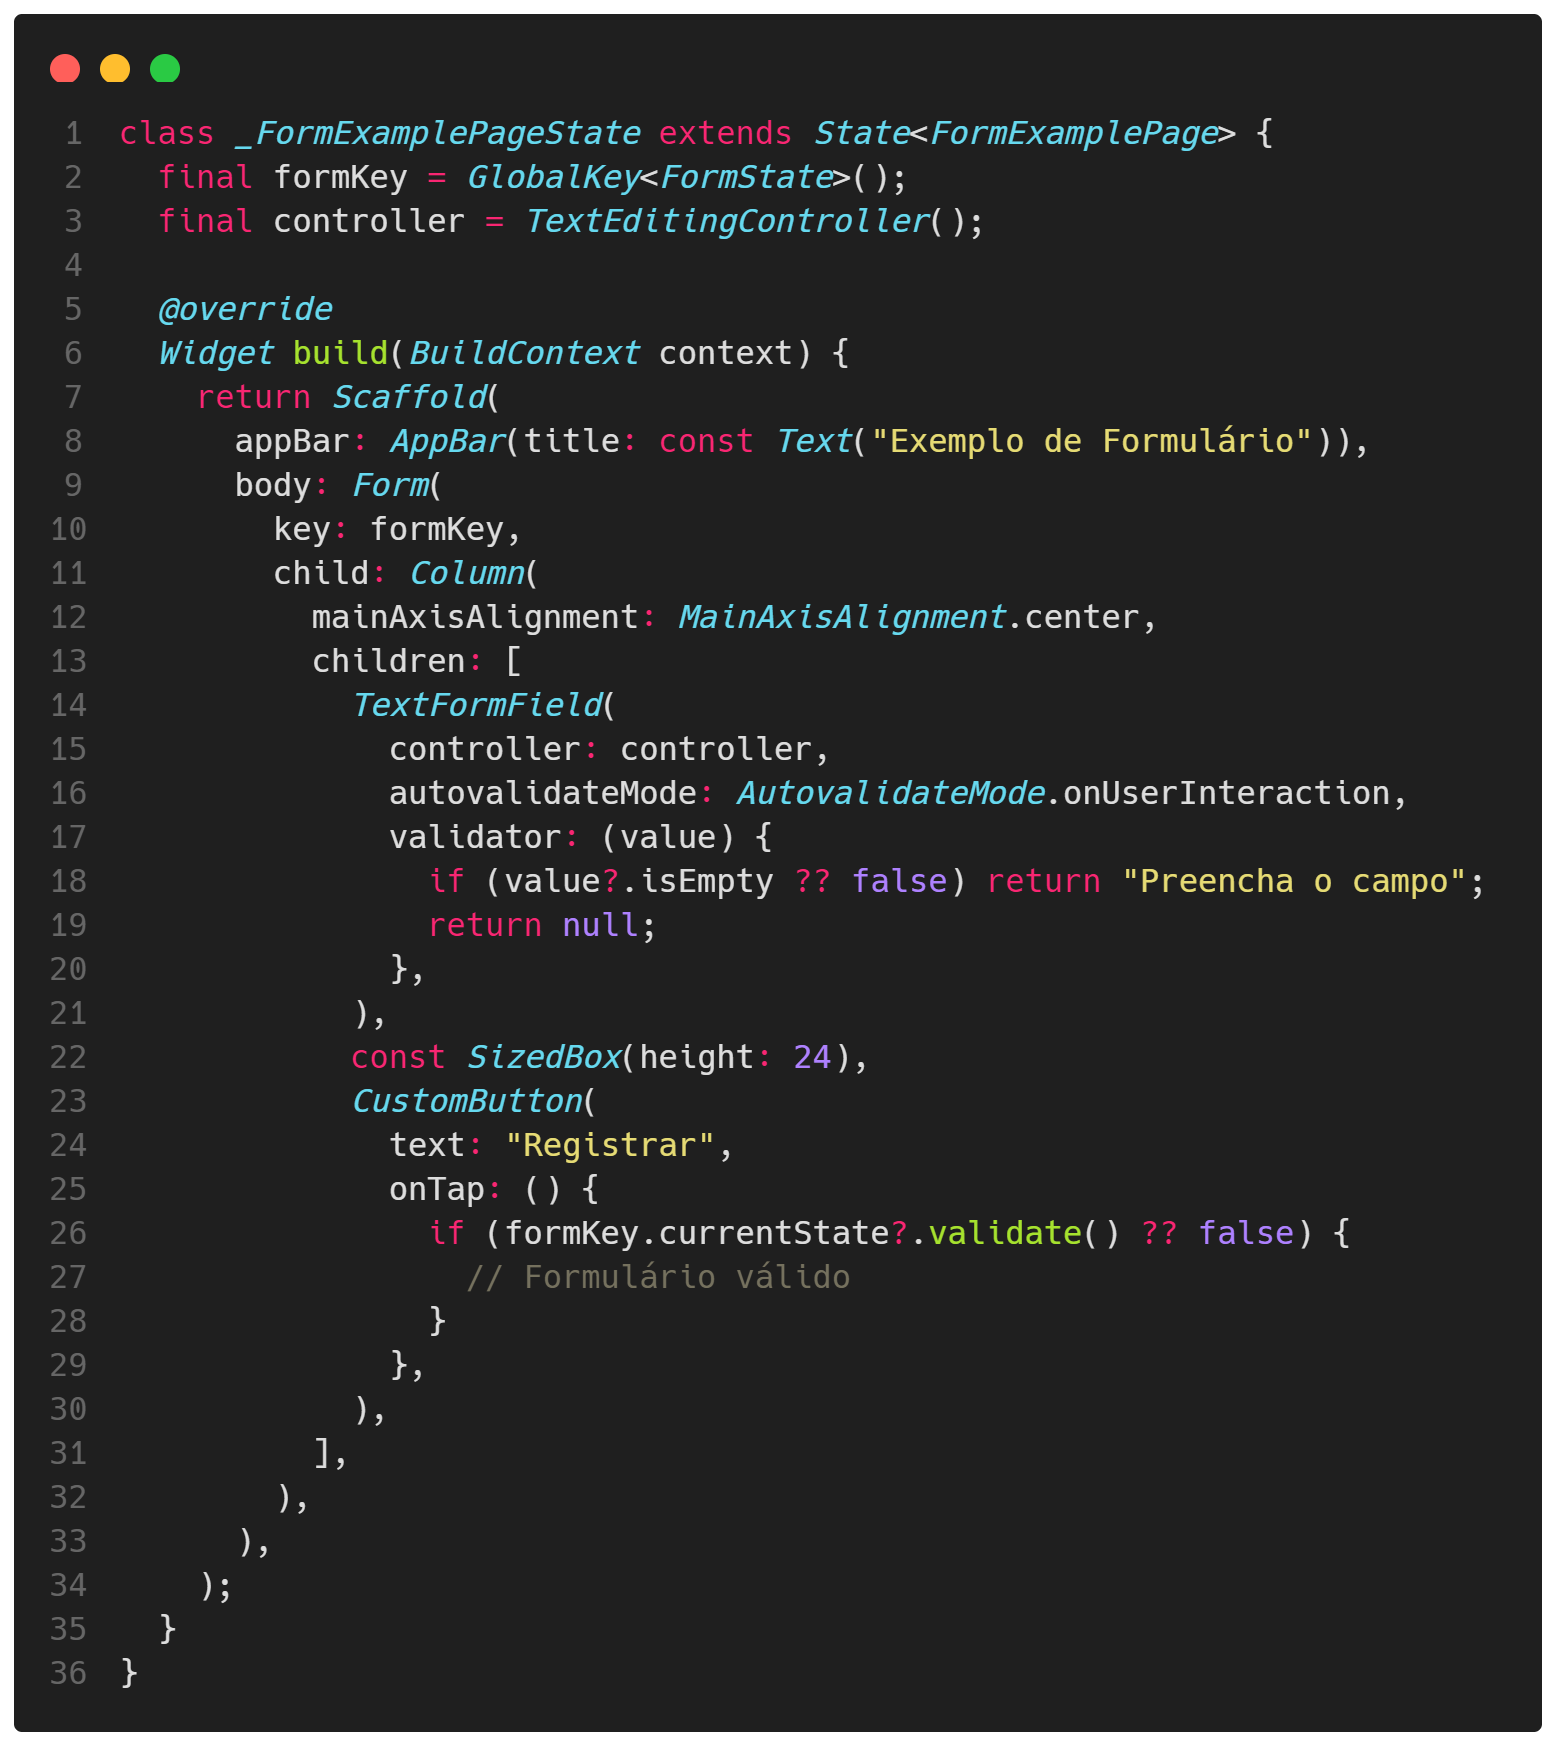
\includegraphics[width=.65\textwidth, trim={0 30 0 100}, clip]{figures/forms/example_form.png}
    \caption{Exemplo de criação de formulário com Flutter}
    \label{fig:example_form}
\end{figure}

Essa abordagem, porém pode apresentar alguns problemas. Para demonstrar esses problemas, e também como resolvê-los por meio da aplicação de padrões de projeto, foi criado um exemplo de formulário com três campos: um para e-mail, que não é obrigatório, mas caso seja preenchido deve ser válido, outro para senha, que é obrigatório e deve ter pelo menos 12 caracteres e pelo menos uma letra e um número, e um campo de confirmação de senha, que é obrigatório e deve verificar se seu conteúdo está idêntico ao campo de senha. Além disso, a tela terá um botão, que só deve estar habilitado caso o formulário esteja válido, como visto nas Figuras \ref{fig:form_preview_invalid} e \ref{fig:form_preview_valid}

\begin{figure}[ht]
    \centering
    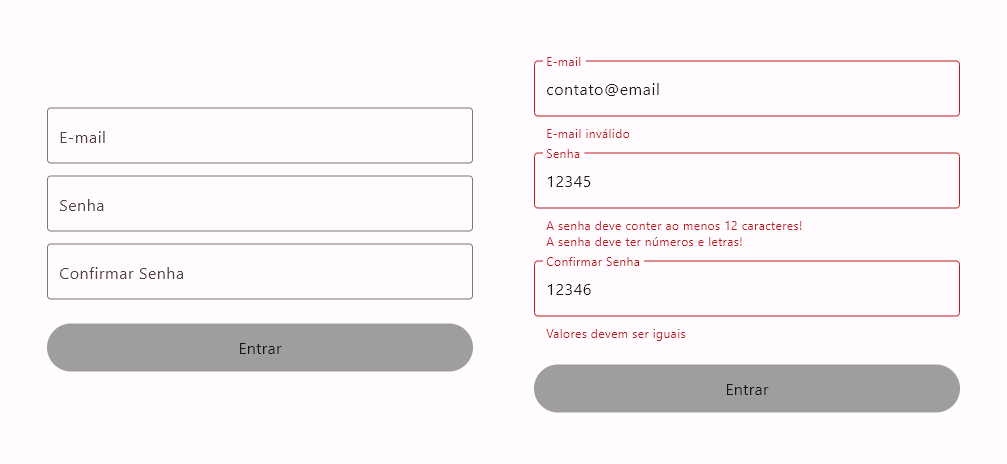
\includegraphics[width=.65\textwidth]{figures/forms/form_preview_invalid.png}
    \caption{Exemplos de formulários inválidos}
    \label{fig:form_preview_invalid}
\end{figure}

\begin{figure}[ht]
    \centering
    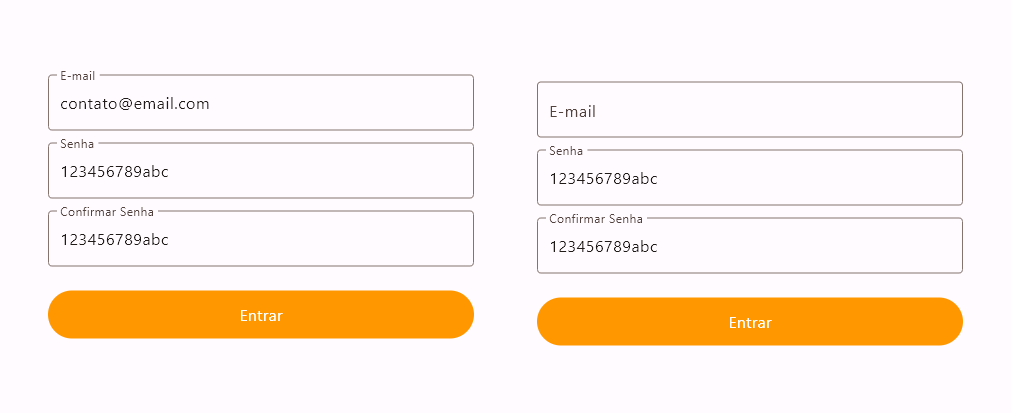
\includegraphics[width=.65\textwidth]{figures/forms/form_preview_valid.png}
    \caption{Exemplos de formulários válidos}
    \label{fig:form_preview_valid}
\end{figure}

A partir do exemplo apresentado na Figura \ref{fig:example_form}, para criar esse formulário de demonstração é necessário criar as funções de validação para cada um dos campos para que seja feita a validação de cada um dos campos, como visto na Figura \ref{fig:form_adhoc_validators}, e adicionar essa função de validação em cada campo, assim como o \textit{TextEditingController} de cada campo, como exemplificado na Figura \ref{fig:form_adhoc_textformfield}. Além disso, para que o botão reaja à validação do formulário, é necessário criar uma variável booleana e uma função que irá verificar se a validação está correta e chamar o método \textit{setState} para atualizar a tela com o novo valor da variável, como na Figura \ref{fig:form_adhoc_checkFields}. Essa função deve ser chamada sempre que houver uma alteração em cada formulário, como é possível visualizar na Figura \ref{fig:form_adhoc_textformfield}

\begin{figure}[ht]
    \centering
    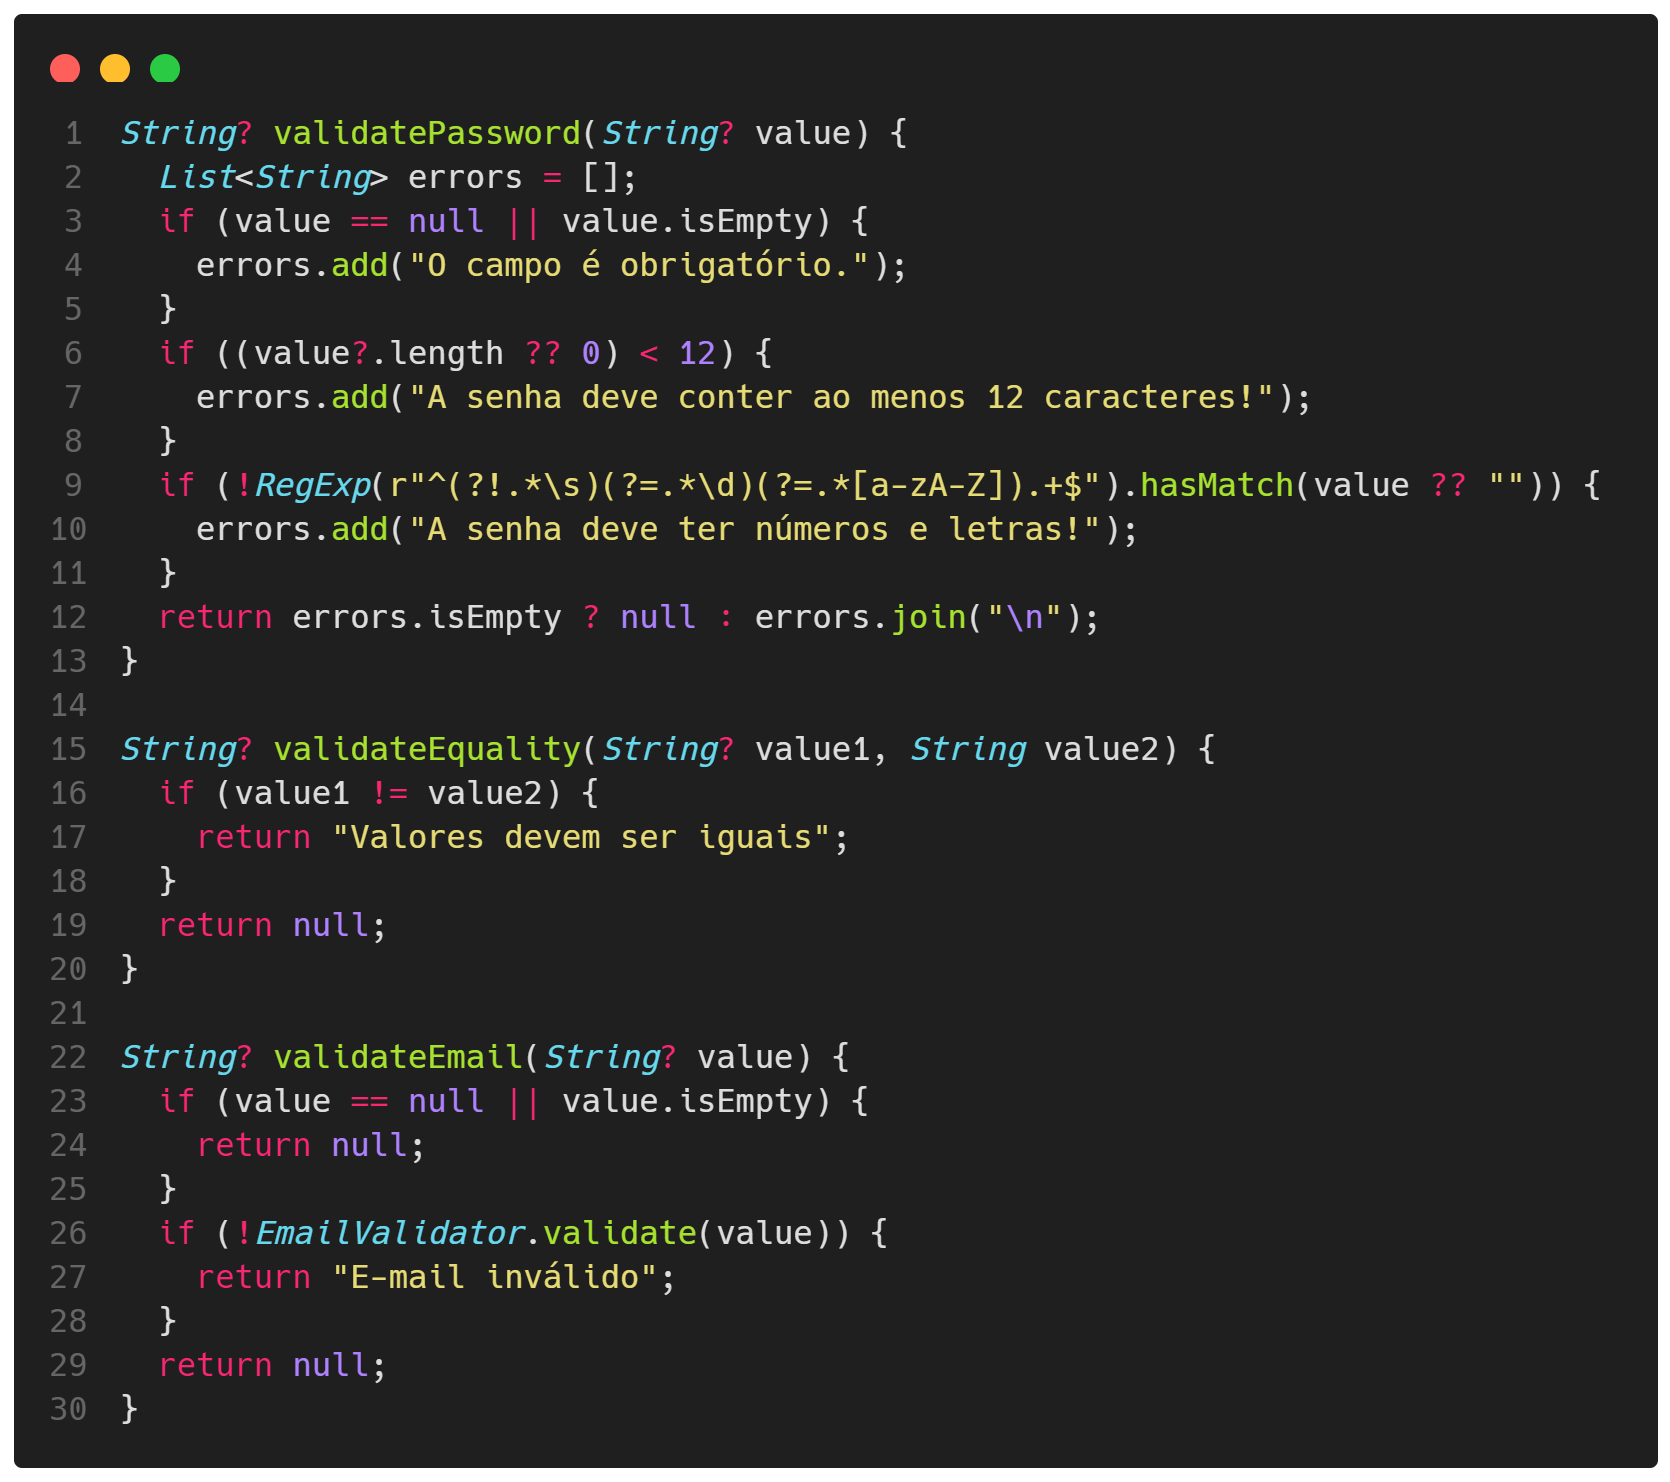
\includegraphics[width=.65\textwidth, trim={0 30 0 100}, clip]{figures/forms/form_adhoc_validators.png}
    \caption{Funções para validação dos campos da demonstração}
    \label{fig:form_adhoc_validators}
\end{figure}

\begin{figure}[ht]
    \centering
    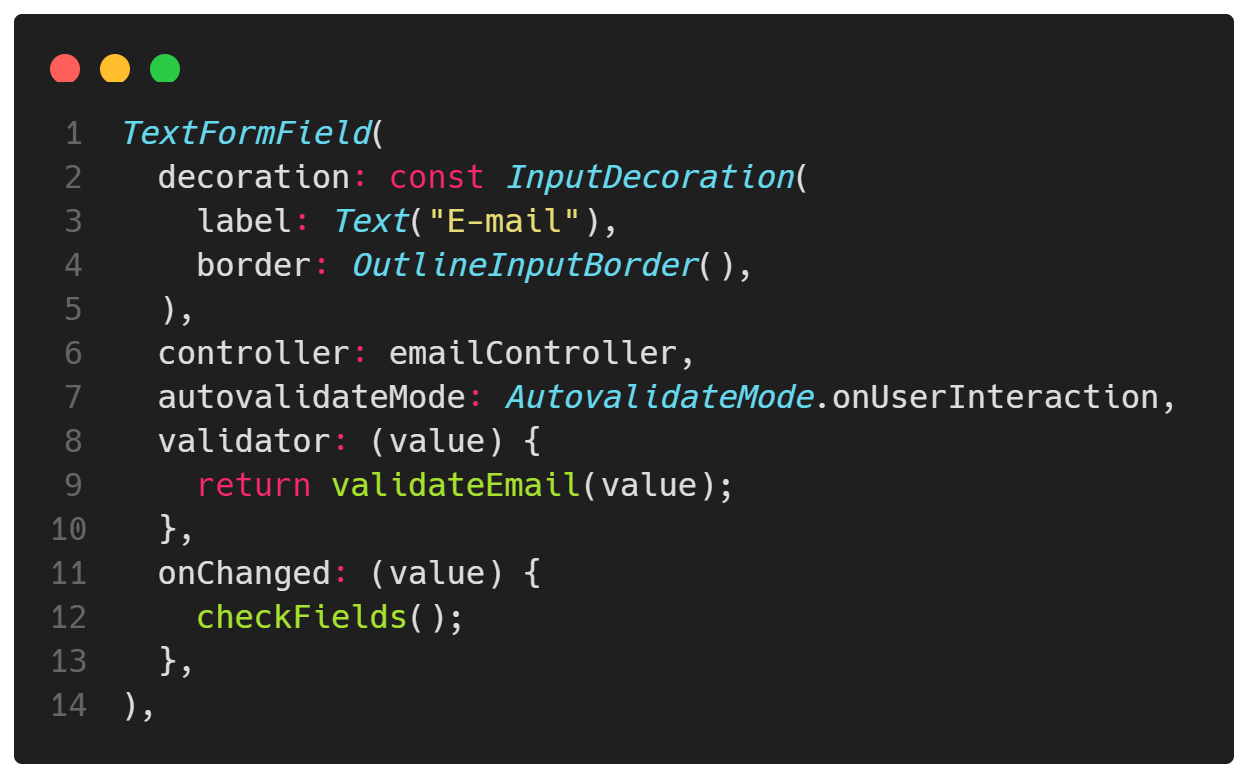
\includegraphics[width=.65\textwidth, trim={0 30 0 100}, clip]{figures/forms/form_adhoc_textformfield.png}
    \caption{Widget TextFormField para o campo de e-mail}
    \label{fig:form_adhoc_textformfield}
\end{figure}

\begin{figure}[ht]
    \centering
    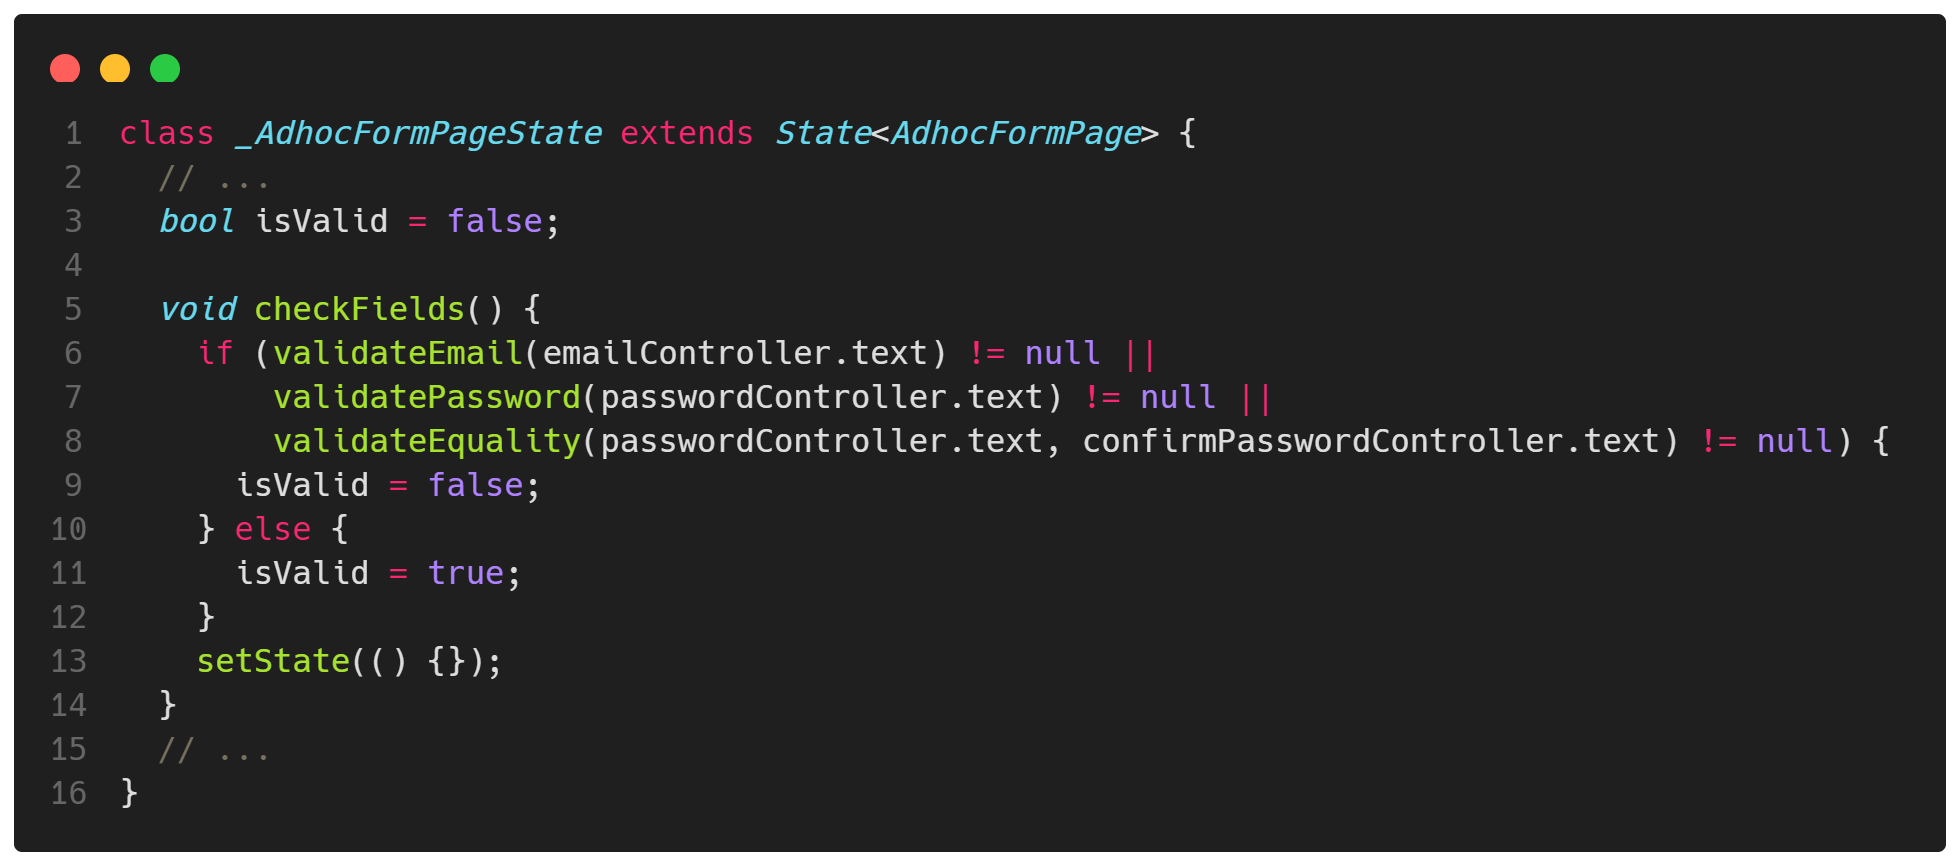
\includegraphics[width=.8\textwidth, trim={0 30 0 100}, clip]{figures/forms/form_adhoc_checkFields.png}
    \caption{Função para verificação da validade}
    \label{fig:form_adhoc_checkFields}
\end{figure}

A partir dessa demonstração inicial, pode-se notar alguns problemas. O primeiro deles é o fato da classe responsável pela tela interface gráfica da aplicação ter que se preocupar também com a validação do formulário, o que sobrecarrega as responsabilidades da classe e fere o Single Responsibility Principle, do SOLID. Um segundo problema é o fato de ter-se que criar explicitamente um \textit{TextEditingController} para cada um dos campos do formulário, o que fará com que tenham muitas variáveis a serem controladas em casos de formulários com muitos campos. Outro porém é a necessidade de chamar a função \textit{checkFields} em cada um dos campos, o que pode ser facilmente esquecido pelo desenvolvedor em algum campo, o que acarretará em um bug na aplicação. Além disso, há o fato de ter-se que chamar as funções de validação duas vezes, o que também pode ser esquecido durante o desenvolvimento e fere o princípio DRY. Um último ponto que é problemático para a escalabilidade da aplicação é o fato das funções de validação serem específicas para o formulário em questão, de forma que é possível que elas não sejam reaproveitáveis em sua totalidade para outros formulários da aplicação. Por exemplo, para o campo e-mail do caso demonstrado não há a validação se o campo é obrigatório. Porém, se em outra parte da aplicação ocorrer de ter um campo e-mail que seja obrigatório teria-se que: ou criar uma nova função, com trecho de código semelhante e, portanto, com duplicação de parte de base de código, ou adicionar um parâmetro booleano na função já existente, o que poderá causar bug em partes da aplicação que já estão desenvolvidas.

\subsection{Aplicação do Padrão Builder em Validadores}

Para resolver o último problema apontado, pode-se aplicar o padrão de projeto Builder, de forma que poderá ser criada a uma classe apenas para lidar com validação de forma mais simplificada. Seguindo o padrão, qualquer parte do código que precisar de fazer uma validação irá especificar, por meio de encadeamento de métodos, quais aspectos do valor de entrada que deseja-se validar e, ao final, chamar um método \textit{build} que irá retornar \textit{null} caso a entrada esteja válida ou uma \textit{String} com a mensagem do que está inválido na dada entrada. A implementação feita, vista na Figura \ref{fig:form_validator} consiste em criar uma classe que recebe em seu construtor a variável do tipo \textit{String nullable} que será feita a validação. Ainda dentro dessa classe, há uma lista de \textit{String} com os erros que podem ser registrados para a entrada dada e também uma variável booleana que indica a obrigatoriedade do campo. Assim, a classe terá uma série de métodos para pequenas validações que serão compostas por quem utilizar a classe, de forma que cada método irá retornar sua própria instância e em caso da entrada ser inválida irá adicionar uma mensagem de erro na lista de erros. Ao final, o método \textit{build} irá retornar \textit{null} caso a lista de erros esteja vazia ou uma \textit{String} que concatenará todos os erros.

\begin{figure}[ht]
    \centering
    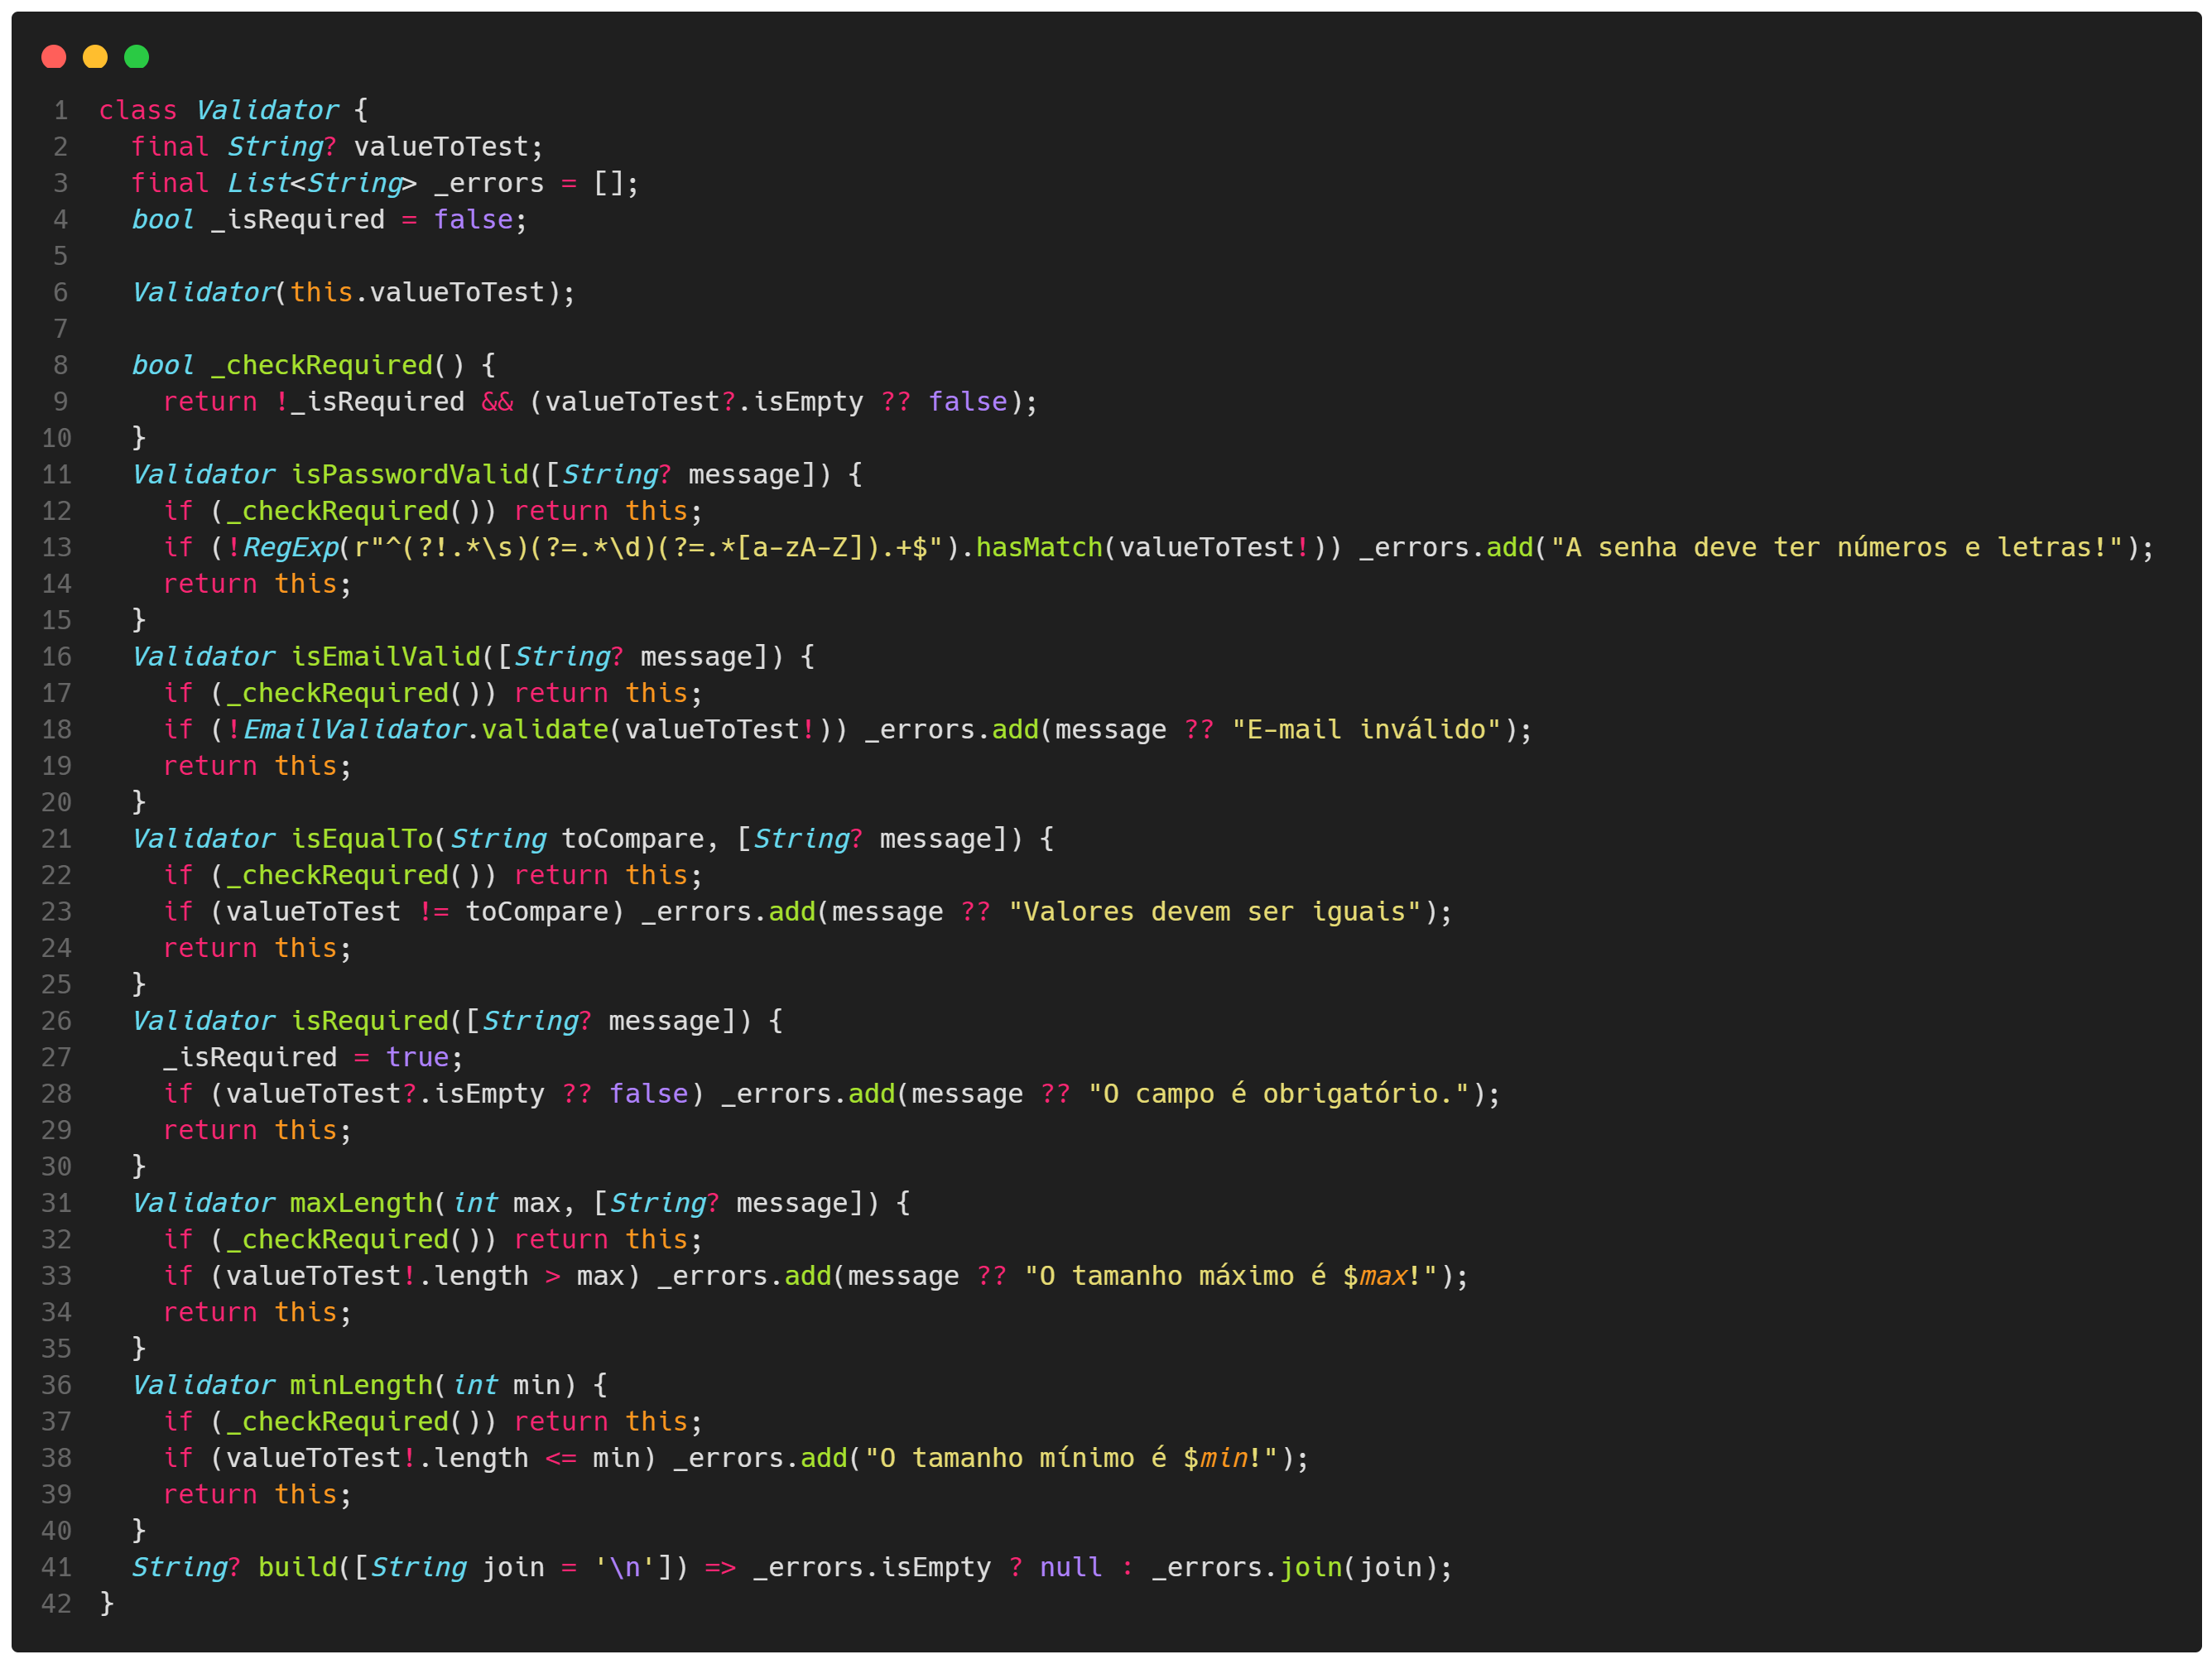
\includegraphics[width=1\textwidth, trim={0 30 0 100}, clip]{figures/forms/form_validator.png}
    \caption{Classe Validator com aplicação do \textit{Builder Pattern}}
    \label{fig:form_validator}
\end{figure}

\subsection{Criação de uma Estrutura para Gerenciamento de Formulários de Forma Facilitada}

Já para resolver os outros problemas apontados, pode-se criar uma nova estrutura separada para lidar apenas com a validação do formulário em si, de forma a isolar toda a lógica de validação da parte da interface gráfica e eliminar as duplicações de código apontadas anteriormente. Além disso, essa nova classe, chamada de \textit{FormManager}, seguirá o padrão de projeto \textit{Observer}, de forma que ela automaticamente irá verificar as alterações nos formulários e indicar aos seus ouvintes se o formulário está em um estado válido ou não.

A implementação da classe \textit{FormManager}, vista na Figura \ref{fig:form_manager} terá como estrutura de dados um \textit{Map<String, FormObject>}, nomeada como \textit{FormsMap}, na qual as chaves serão uma \textit{String} com um identificador para o campo e o valor armazenado será uma instância da classe \textit{FormObject}, que as seguintes propriedades:

\begin{itemize}
    \item \textit{label}, que será o texto a ser exibido na tela para cada campo do formulário;
    \item \textit{validator}, que será o método \textit{build} da classe \textit{Validator} criada anteriormente;
    \item \textit{controller}, que será uma instância de \textit{TextEditingController} a ser criada pelo próprio \textit{FormManager};
    \item \textit{onChange}, que será uma função a ser chamada a cada vez que houver modificação em um campo do formulário, também gerenciada pela própria classe \textit{FormManager};
\end{itemize}

Além dessa estrutura de dados, a classe \textit{FormManager} terá o método \textit{setForms}, que irá receber um \textit{Map<String, FormObjectParameters>}, em que o \textit{FormObjectParameters} é possui apenas os atributos \textit{label} e \textit{validator} da classe \textit{FormObject}. Esse método irá passar por todas as entradas do mapa passado e irá adicionar uma nova entrada na estrutura de \textit{FormsMap}, de forma a criar o \textit{TextEditingController} para cada campo e definir a função anônima a ser chamada quando o campo for alterado. Essa função anônima chamará a função privada \textit{\_checkIsValid} que passará por toda a estrutura de dados \textit{FormsMap} e checará se o valor atual do campo, provido pelo atributo \textit{controller}, está válido. Caso todos estejam válidos, atribuirá o valor verdadeiro para a variável \textit{\_isValid}, caso contrário, atribuirá o valor falso. Após a chamada desse método privado, será chamado o método herdado da classe \textit{Notifier}, \textit{notifyListeners}, que irá avisar a todos os ouvintes sobre o novo estado da classe.

\begin{figure}[ht]
    \centering
    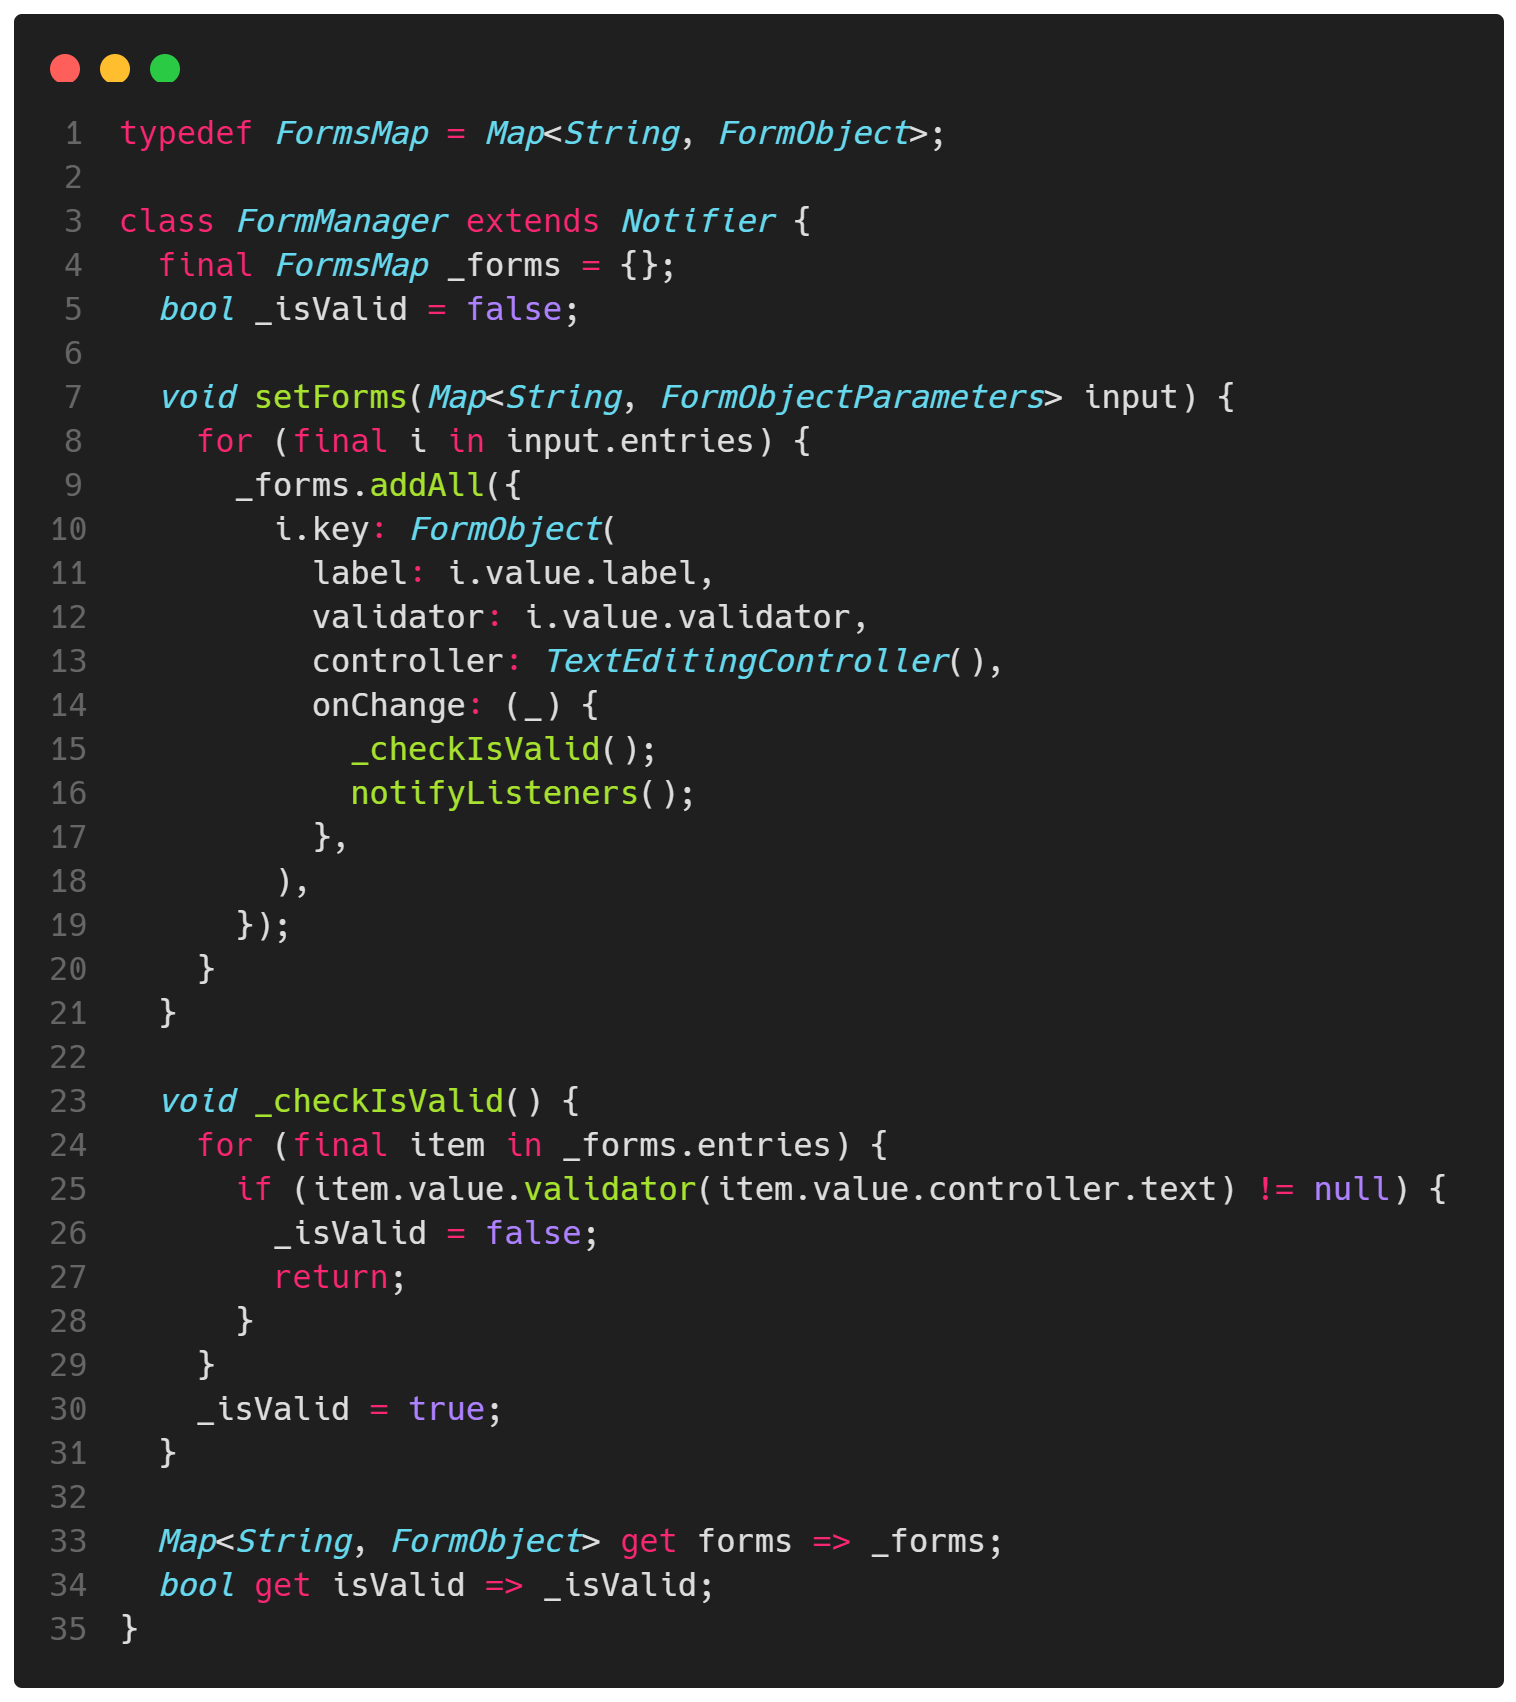
\includegraphics[width=.7\textwidth, trim={0 30 0 100}, clip]{figures/forms/form_manager.png}
    \caption{Classe \textit{FormManager}, responsável por encapsular todo o registro e validação dos formulários}
    \label{fig:form_manager}
\end{figure}

Assim, como o \textit{FormManager} criado, pode-se criar uma nova instância dele na classe da UI e, na inicialização da tela, por meio do método \textit{initState}, definir quais os campos do formulário e quais serão as validações feitas sobre eles, como demonstrado na Figura \ref{fig:set_forms}. Essa forma de criar formulários, além de ser menos passível de erros por descrever-se as validações apenas uma vez, é muito mais semântica, já que deixa explícito o que está sendo validado em cada campo.

\begin{figure}[ht]
    \centering
    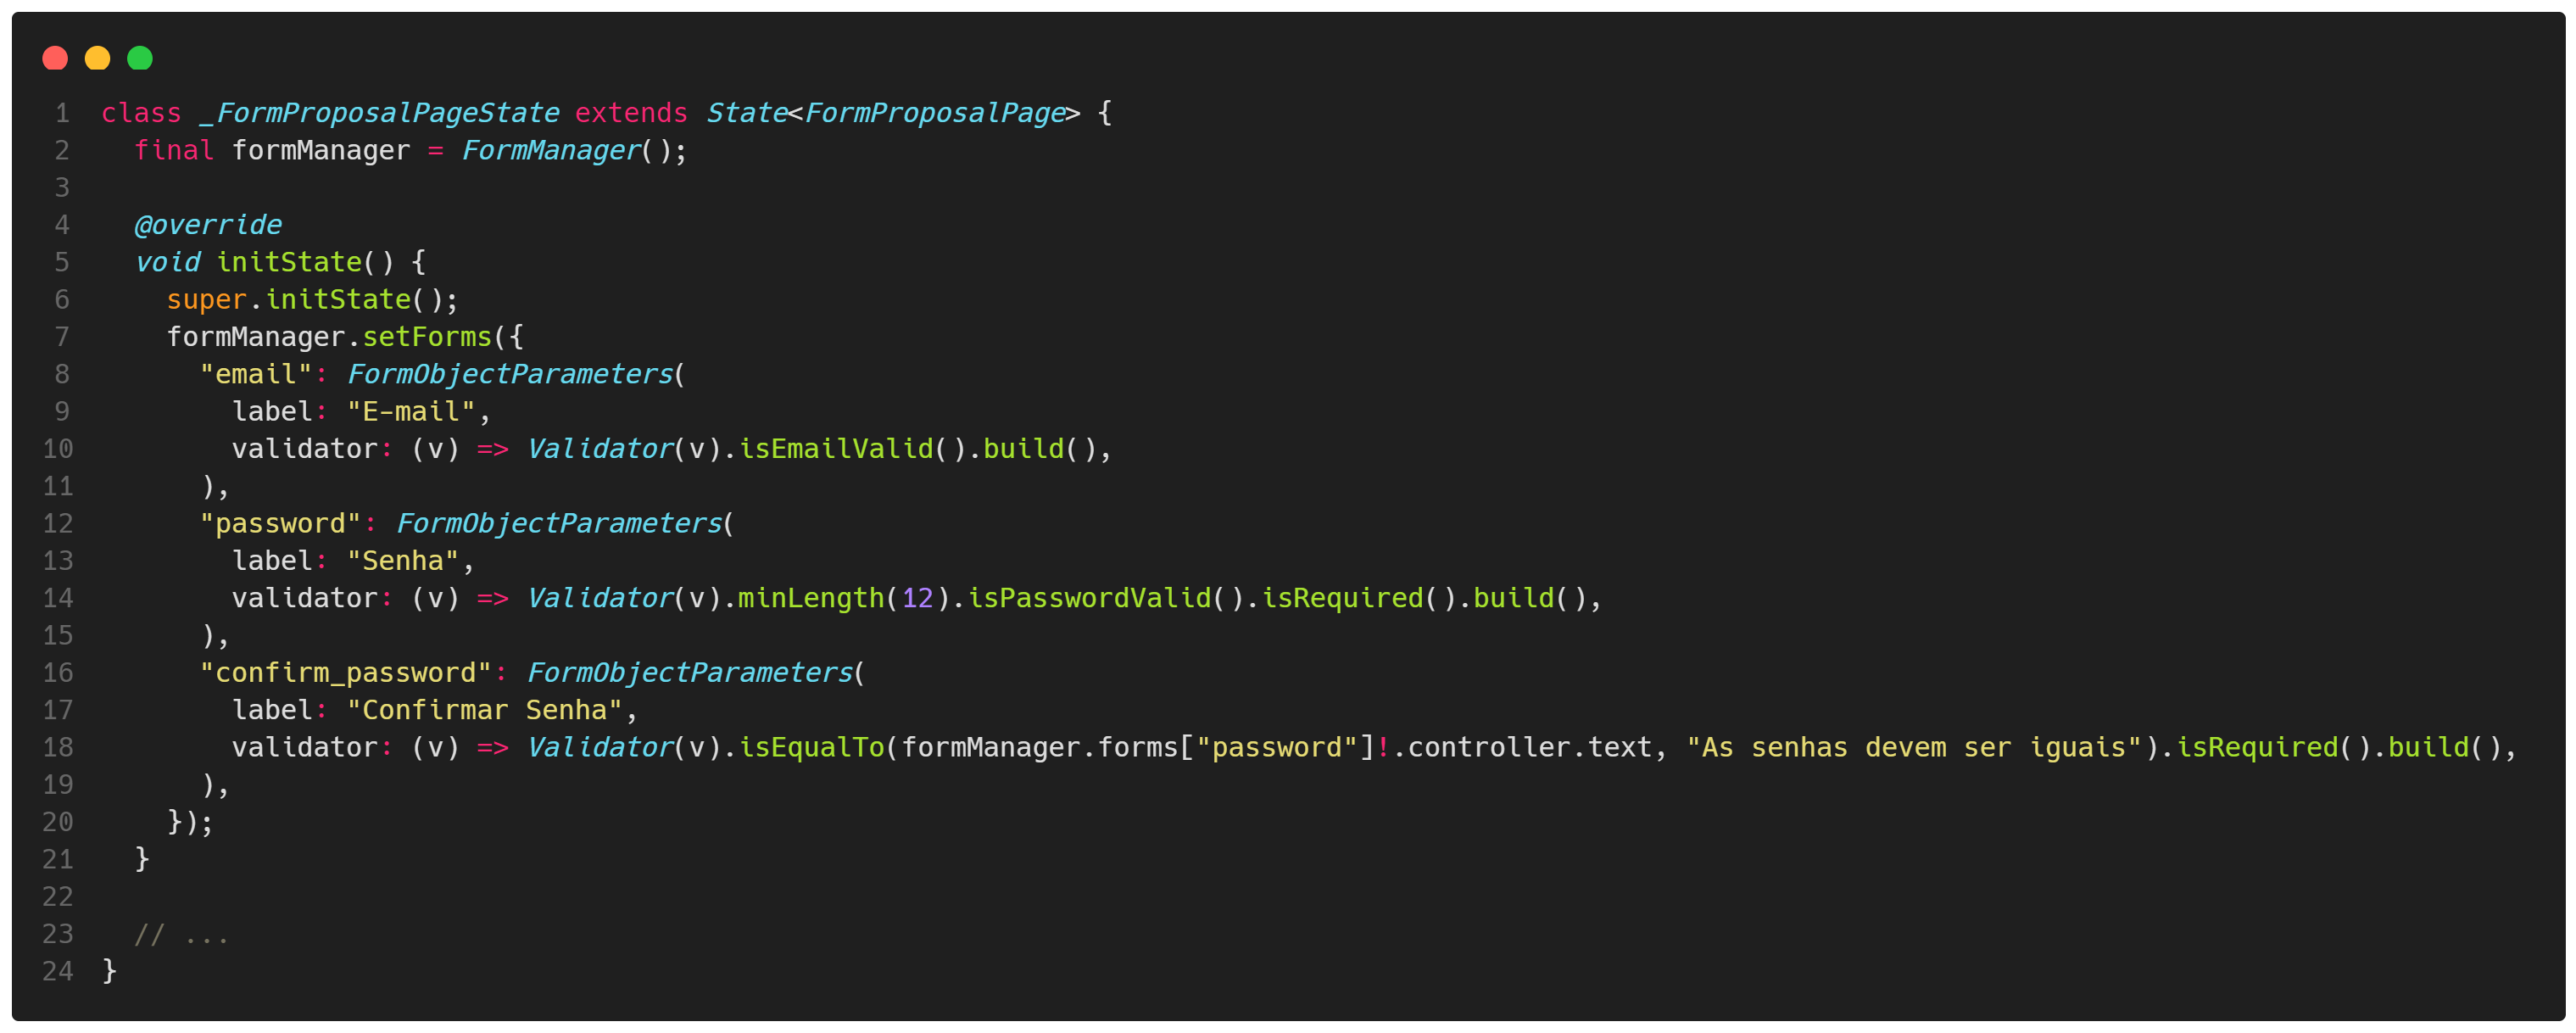
\includegraphics[width=1\textwidth, trim={0 30 0 100}, clip]{figures/forms/set_forms.png}
    \caption{Inicialização dos formulários na tela}
    \label{fig:set_forms}
\end{figure}

Para terminar o uso das novas estruturas criadas, basta passar as informações do \textit{FormManager} para os componentes da interface. Nisso, o \textit{TextFormField} terá que receber os parâmetros \textit{label}, \textit{controller}, \textit{validator} e \textit{onChange} em cada campo. Além disso, para customizações visuais nos campos de formulário, como adição de ícones e customização de fonte, teria-se que repetir grandes trechos de código. Para evitar essa duplicação desnecessária, pode-se criar um componente customizado para o formulário, como visto na Figura \ref{fig:custom_text_field}.

\begin{figure}[ht]
    \centering
    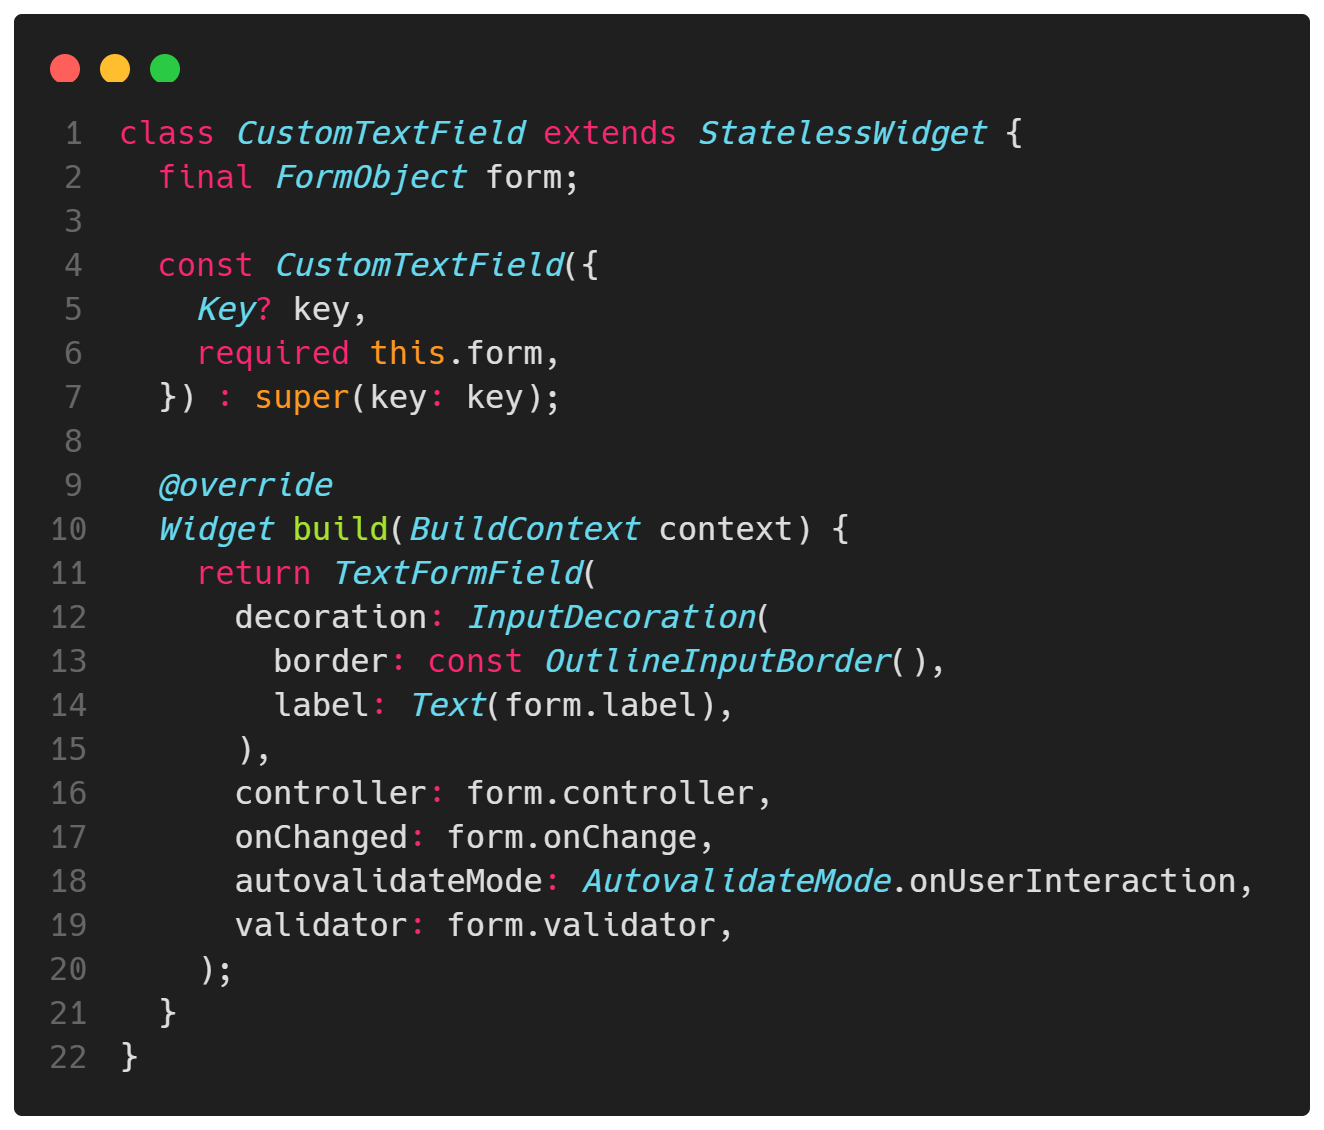
\includegraphics[width=.65\textwidth, trim={0 30 0 100}, clip]{figures/forms/custom_text_field.png}
    \caption{Criação do componente personalizado para um formulário}
    \label{fig:custom_text_field}
\end{figure}

Assim, o uso de todas essas classes será o presente na Figura \ref{fig:use_of_form_proposal}, em que terá-se um \textit{NotifierBuilder} para notificar os componentes sobre as alterações do \textit{FormManager} e será listado de forma direta quais os campos existentes para aquele formulário, além de o widget \textit{CustomButton} já saber sempre se o estado do formulário é válido ou não para bloquear ou não o clique sobre o botão.

\begin{figure}[ht]
    \centering
    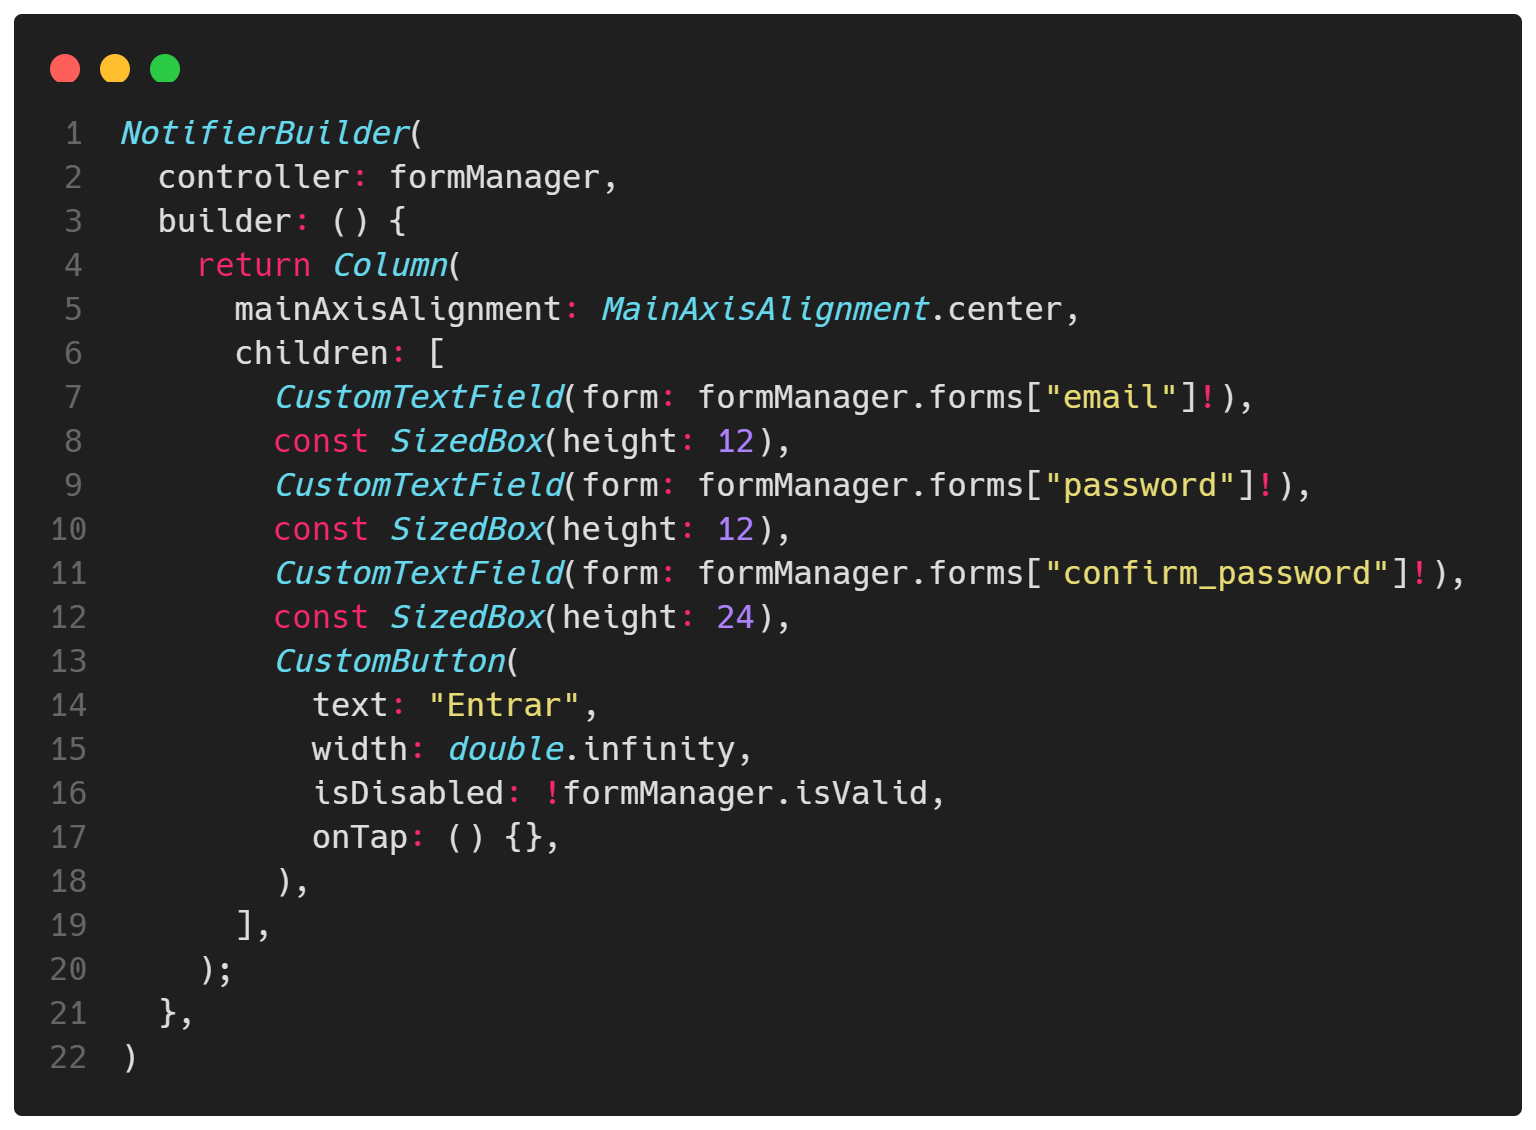
\includegraphics[width=.65\textwidth, trim={0 30 0 100}, clip]{figures/forms/use_of_form_proposal.png}
    \caption{Uso dos formulários com reatividade no código da interface gráfica}
    \label{fig:use_of_form_proposal}
\end{figure}


\section{Apresentação de Componentes de Plataformas Específicas de Forma Facilitada}

Em termos de identidade visual, cada sistema operacional possui seu próprio \textit{Design System}, que corresponde a um conjunto de componentes prontos que seguem um padrão estabelecido por uma organização. Assim, têm-se que a \textit{Google} possui o \textit{Material Design}, a \textit{Apple} em seus SOs possui o \textit{Human Interface Guidelines}, a \textit{Microsoft} com o \textit{Windows} possui a \textit{Fluent UI}, dentre outros. Com isso, no momento de desenvolver uma aplicação cliente utilizando o Flutter, têm-se duas opções no que tange à construção de interfaces gráficas. Pode-se optar por criar um \textit{Design System} próprio para a aplicação, de forma que ele seja totalmente customizável e tenha um mesmo comportamento em todas as plataformas em que a aplicação irá rodar. Essa escolha colabora com a aplicação ter uma identidade visual mais forte, porém num momento inicial os usuário podem ficar perdidos pelo fato da interface não ser muito semelhante à interface do sistema operacional que usam, necessitando de um tempo para se acostumarem.

Uma outra opção é de fazer com que o layout da aplicação seja único para cada plataforma, seja em sua totalidade, seja em componentes específicos que o \textit{Design System} do SO já possui um componente que realiza a função desejada. Para aplicações nativas, essa tarefa se torna trivial, visto que um desenvolvedor \textit{Android}, que irá criar uma aplicação em Kotlin e possui acesso apenas ao \textit{Material Design} da Google para a criação dos componentes. O mesmo é válido para desenvolvedores \textit{iOS}, que já possuirão todas as ferramentas fornecidas pela Apple e conseguirão apenas criar aplicações para o ecossistema da Apple.

Porém, para desenvolvedores que utilizam de \textit{frameworks cross-platform}, como o Flutter, para adotar essa segunda abordagem seria necessário em todo componente que se deseje ter a aparência da plataforma em que o app está rodando, fazer verificações sobre qual plaforma a aplicação está sendo utilizada, o que levará a duplicação em diversas partes da base de código. Assim, de forma a seguir o princípio DRY, essa  seção desse trabalho propõe em utilizar o padrão de projeto \textit{Factory} para resolver essa problemática. Será desenvolvida uma prova de conceito simples que mostrará um componente \textit{Dialog} ao apertar de uma botão, de forma que ele seguirá o \textit{Material Design} quando a aplicação estiver no \textit{Android} e seguirá o \textit{Cupertino Design System} quando estiver rodando no \textit{iOS}, como mostrado na Figura \ref{fig:plaforms_dialog}

\begin{figure}[ht]
    \centering
    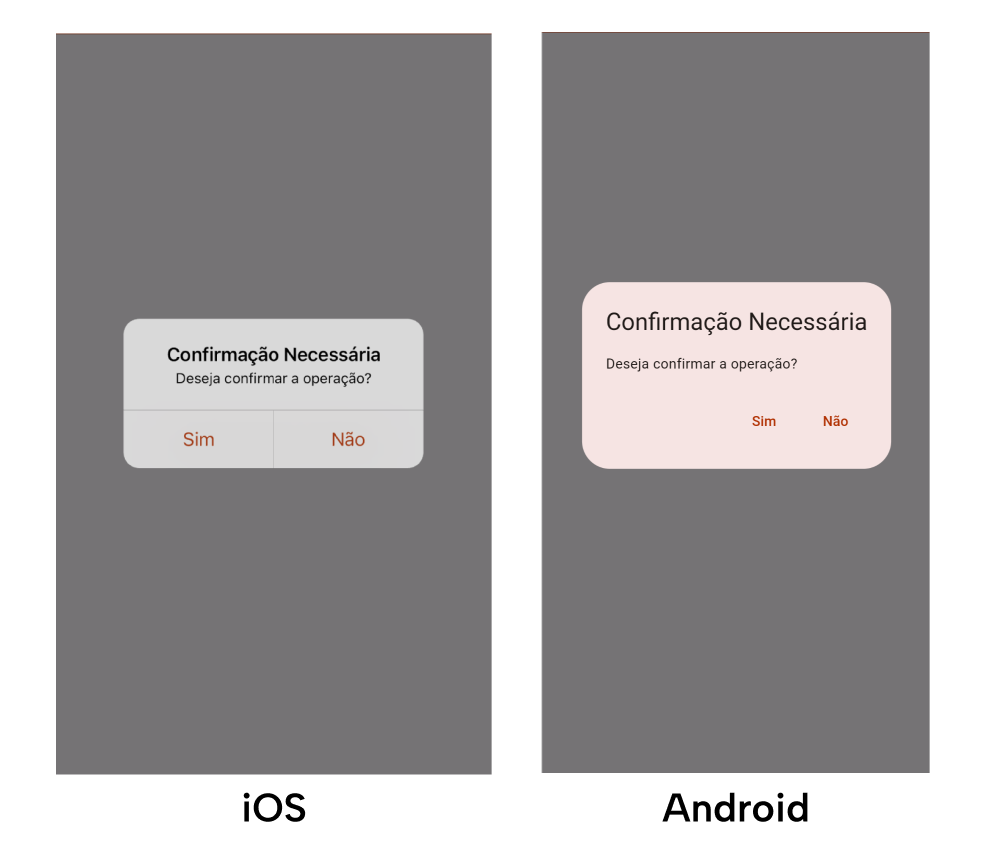
\includegraphics[width=.65\textwidth]{figures/dialog/platforms_dialog.png}
    \caption{Exemplo da visualização dos Dialog no iOS e Android, respectivamente}
    \label{fig:plaforms_dialog}
\end{figure}

\subsection{Forma Direta de Apresentar Componentes Nativos}

Para a exibição de \textit{Dialogs}, o Flutter disponibiliza a função assíncrona \textit{showDialog}, que recebe o \textit{BuildContext} e uma função que retornará um widget a ser exibido. Esse widget será o \textit{CupertinoAlertDialog} para o \textit{iOS} e um \textit{AlertDialog} para o \textit{Android}, ambos providos pelo próprio Flutter, de forma que será necessário chamar métodos estáticos da classe \textit{Platform}, da biblioteca \textit{dart:io} para verificar em qual SO a aplicação está rodando, como mostrado na Figura \ref{fig:adhoc_dialog}

\begin{figure}[ht]
    \centering
    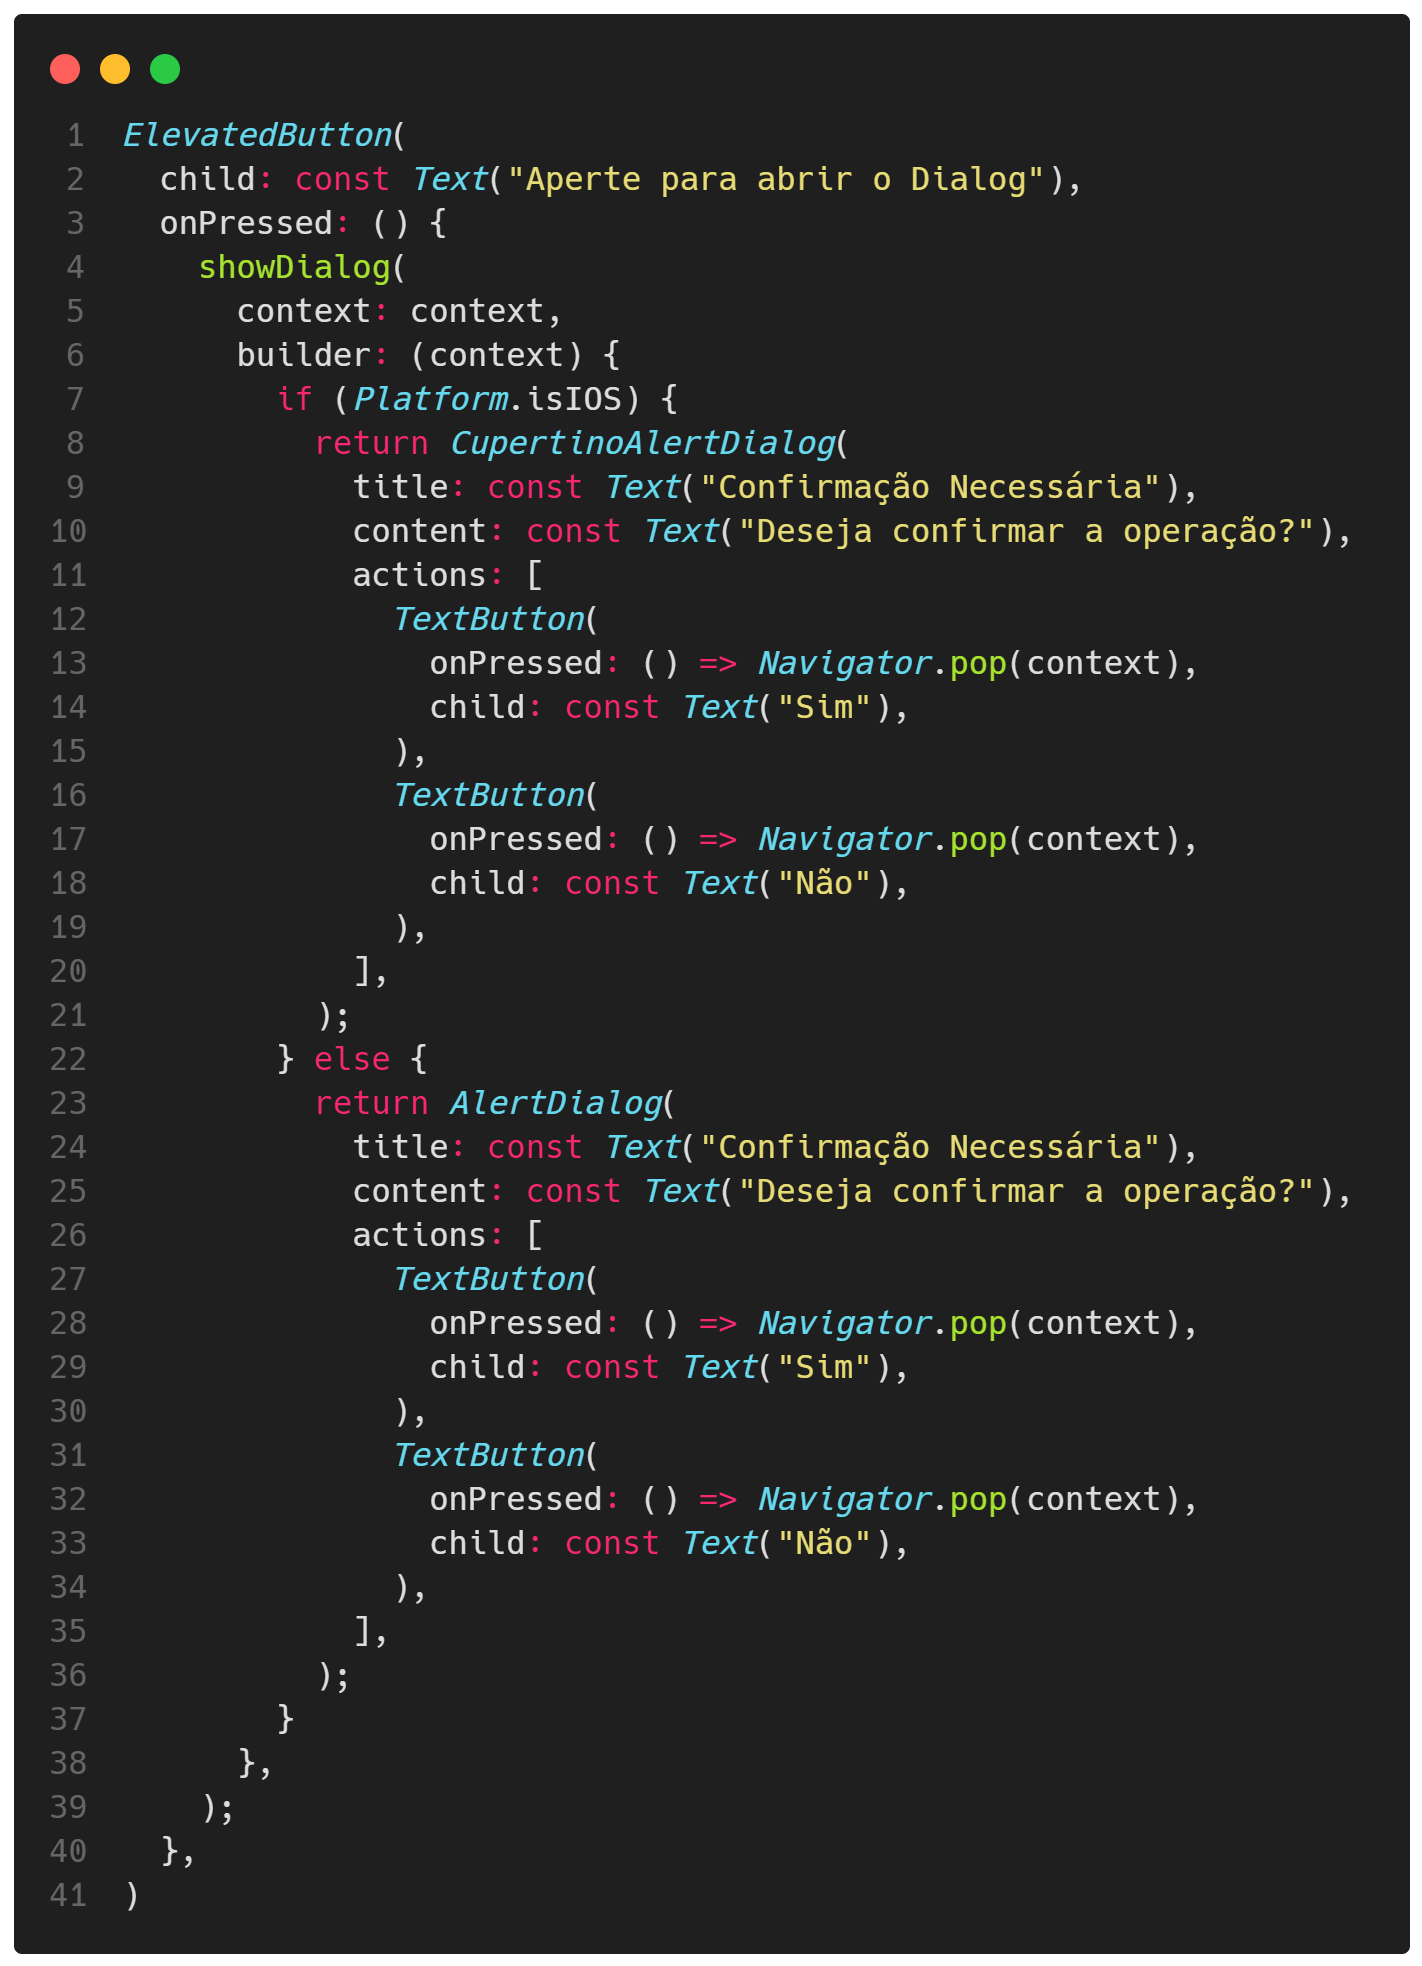
\includegraphics[width=.65\textwidth, trim={0 30 0 100}, clip]{figures/dialog/adhoc_dialog.png}
    \caption{Exemplo direto do uso de diferentes Dialogs de acordo com o SO no qual a aplicação está rodando}
    \label{fig:adhoc_dialog}
\end{figure}

Apesar de bem direta, a forma apresentada acarretará em problemas futuros para o projeto, visto que haverá sempre a duplicação de código ao chamar as classes \textit{AlertDialog} e \textit{CupertinoAlertDialog} em vários lugares na base de código, de forma que caso o Flutter mude os parâmetros dessas classes em versões futuras, ou até mesmo descontinue a classe em favor de outra, seria necessário fazer alterações em vários arquivos do projeto. Além disso, têm-se o fato de sempre ser necessária as verificações de plataforma em todo lugar que for necessário exibir o \textit{Dialog}, de forma que se em um futuro a aplicação passar a dar suporte a uma nova plataforma, será necessário ir em todas as checagens e adicionar uma nova condição para essa nova plataforma para que seja exibido um novo componente.

\subsection{Uso do Padrão Factory para Mostrar Componentes Nativos}

Diante dos problemas apresentados, é possível introduzir o padrão de projeto \textit{Factory}, que permitirá a criação de uma classe que encapsulará a responsabilidade de realizar a checagem de plataforma e, diante de uma interface criada para a exibição de \textit{Dialogs}, irá retornar o \textit{Dialog} apropriado para a plataforma vigente em que a aplicação está rodando. Para implementar esse padrão, é necessário primeiramente criar a interface que todas as implementações de \textit{Dialog} devem seguir. Essa interface receberá o título, conteúdo e as ações possíveis para os botões do \textit{Dialog}, como visto na Figura \ref{fig:base_dialog}

\begin{figure}[ht]
    \centering
    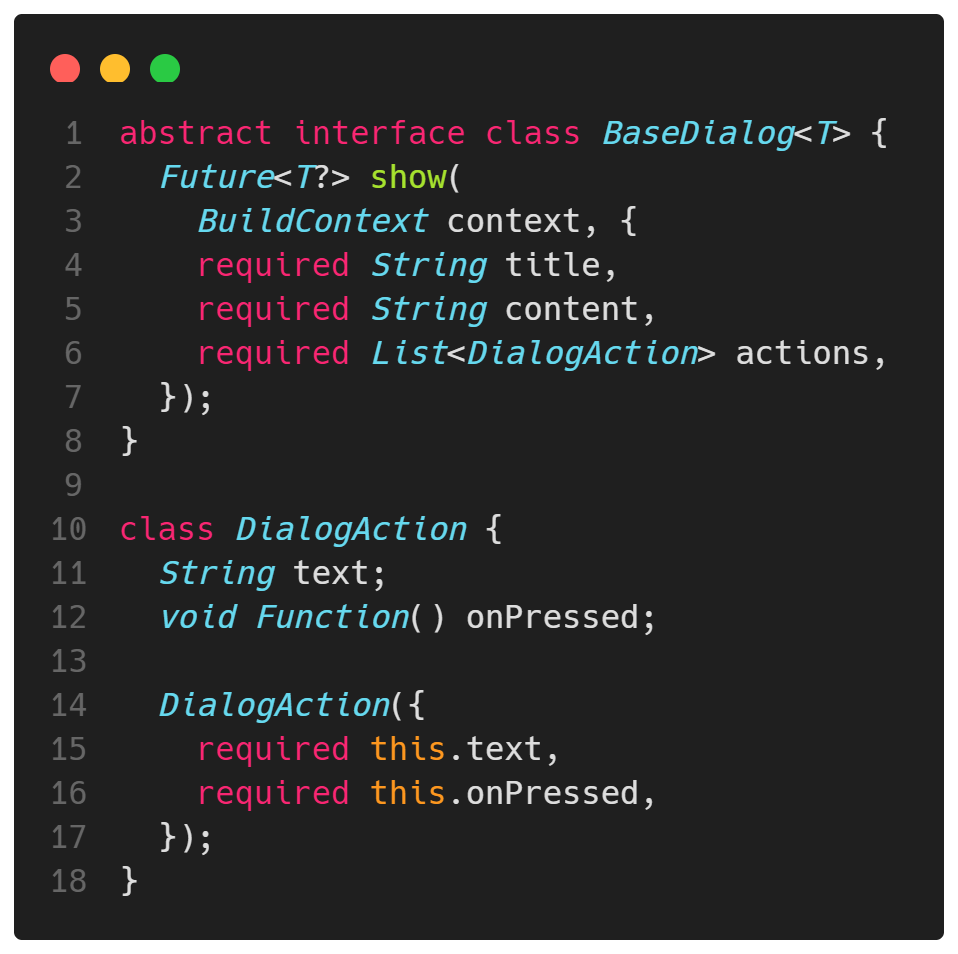
\includegraphics[width=.85\textwidth, trim={0 30 0 100}, clip]{figures/dialog/base_dialog.png}
    \caption{Interface para criação de Dialogs}
    \label{fig:base_dialog}
\end{figure}

Em seguida, deve-se criar as implementações dos \textit{Dialogs} a partir dessa interface criada, com cada um retornando o componente correto de cada plataforma e realizando customizações que serão específicas daquela plataforma, como visto na Figura \ref{fig:dialog_implementations}


\begin{figure}[ht]
    \centering
    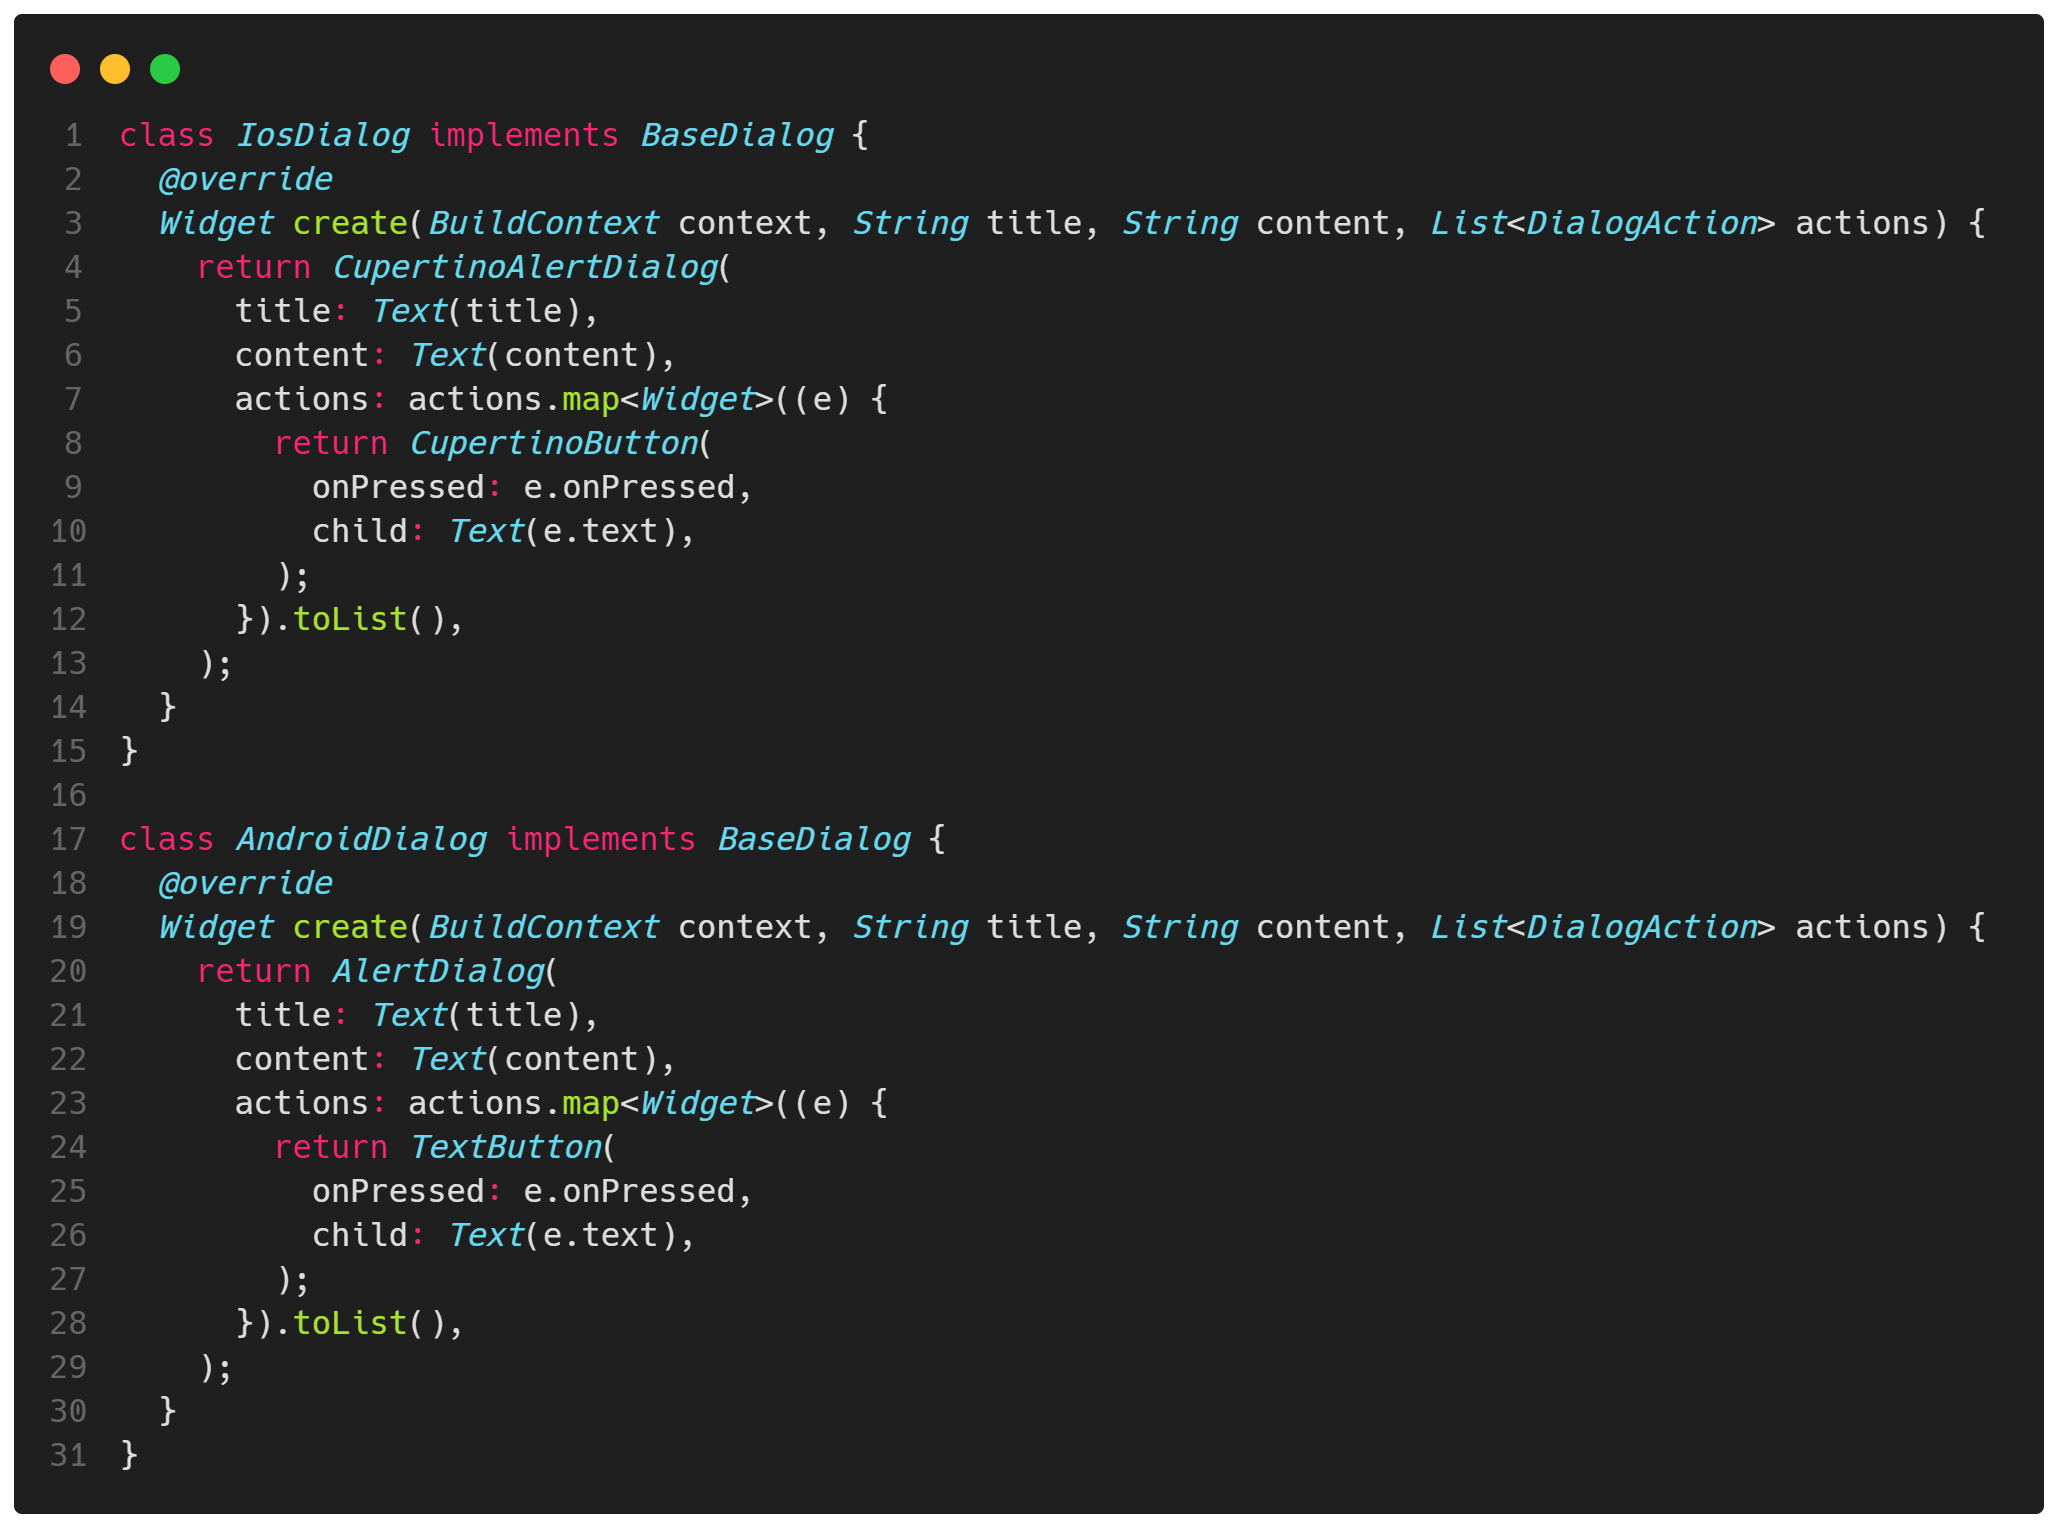
\includegraphics[width=.85\textwidth, trim={0 30 0 100}, clip]{figures/dialog/dialog_implementations.png}
    \caption{Implementações dos \textit{Dialogs} com base na interface \textit{BaseDialog}}
    \label{fig:dialog_implementations}
\end{figure}

Por último, deve-se criar a classe \textit{DialogFactory}, que irá receber os parâmetros de título, conteúdo e ações dos botões e irá fazer a verificação de qual plataforma a aplicação está rodando para que possa ser feita a escolha de qual implementação do \textit{BaseDialog} será utilizada para a exibição do componente de \textit{dialog}, como visto na Figura \ref{fig:dialog_factory}. Com essa implementação utilizando o padrão \textit{Factory}, quando for necessário adicionar uma nova plataforma, bastará criar a nova implementação da interface \textit{BaseDialog} e adicionar uma única nova condição dentro da fábrica, de forma em qualquer lugar da base de código que chame o método estático \textit{showAlertDialog} já será exibido o componente correto para a nova plataforma. Destaca-se que esse padrão pode ser aplicado para qualquer parte da interface, desde partes que chamem componentes de interface comuns nos sistemas operacionais, como \textit{overlays} de carregamento, \textit{date pickers}, \textit{dialogs}, até componentes mais específicos da aplicação em si, como \textit{cards}, campos de texto, botões, etc.

\begin{figure}[ht]
    \centering
    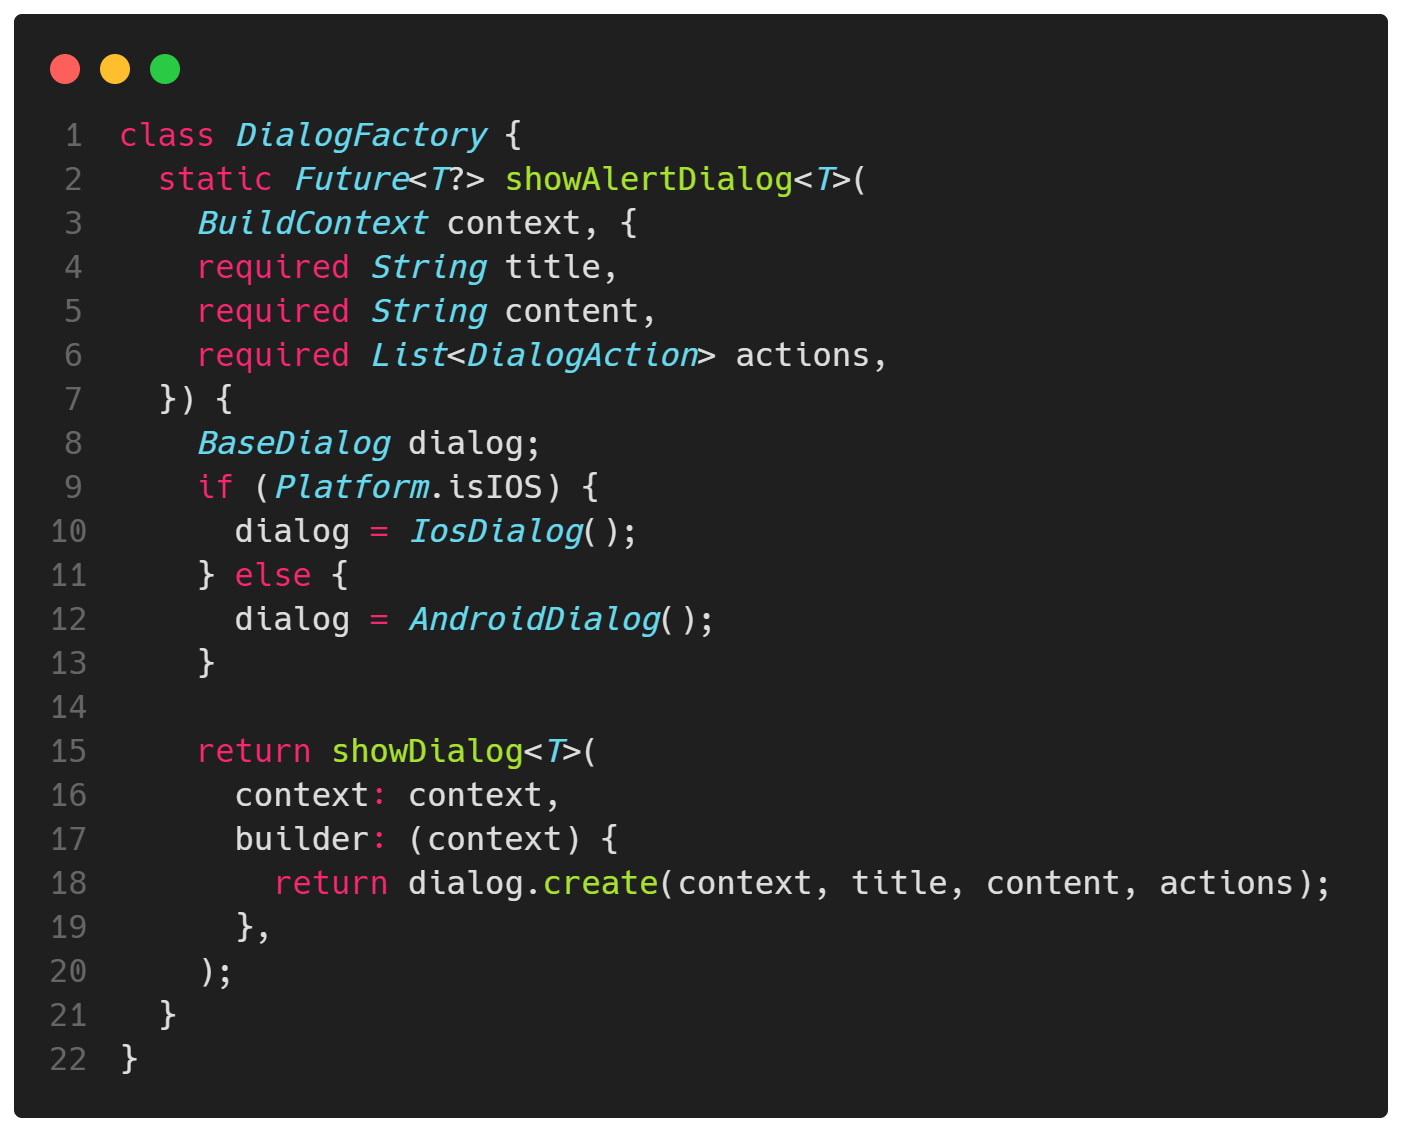
\includegraphics[width=.85\textwidth, trim={0 30 0 100}, clip]{figures/dialog/dialog_factory.png}
    \caption{Classe que utiliza propriamente o padrão \textit{Factory}}
    \label{fig:dialog_factory}
\end{figure}


\section{Aplicação de Conceitos de Arquitetura de Software em Aplicações Flutter}


\subsection{Uma Aplicação Clássica da Arquitetura Limpa}

\subsection{Aplicações Offline-First: Uma Responsabilidade da Camada de Infraestrutura}

\subsection{Uma Arquitetura de Duas Camadas Simplificada}
% Application Bussiness Rules da CleanArch são muito atrelados à tela

\chapter{Conclusão}

% ----------------------------------------------------------
% ELEMENTOS PÓS-TEXTUAIS
% ----------------------------------------------------------
\postextual


% ----------------------------------------------------------
% Referências bibliográficas
% ----------------------------------------------------------
\bibliography{abntex2-modelo-references}

\end{document}